% Statistics MCQ question bank: First Paper + Second Paper.
% This is the single source file. Add, edit and reorder questions here.
% Compile from question/ (twice, for the table of contents):
%   pdflatex stat_mcq_bank.tex
%
% Image paths are relative to question/.
% build_quiz.py splits the papers at the "PAPER 1" / "PAPER 2" comment lines; keep them.
\documentclass{exam}
\usepackage{amsmath,amsthm,amsfonts,amssymb,dsfont}
\usepackage{ifthen}
\usepackage{enumerate}% http://ctan.org/pkg/enumerate
\usepackage{multicol}
\usepackage{graphicx}
\usepackage{float}
\usepackage{xcolor}
\usepackage{lipsum}
\usepackage{hyperref}

% Accumulate the answers. Unmodified from Phil Hirschorn's answer
% https://tex.stackexchange.com/questions/15350/showing-solutions-of-the-questions-separately/15353
\newbox\allanswers
\setbox\allanswers=\vbox{}

\newenvironment{answer}
{%
    \global\setbox\allanswers=\vbox\bgroup
    \unvbox\allanswers
    % set each answer at the width of a key column (3 columns), so long ones wrap
    \hsize=\dimexpr(\textwidth-2\columnsep)/3\relax
    \linewidth=\hsize
    \parshape=0 \leftskip=0pt \raggedright
}%
{%
    \bigbreak
    \egroup
}

\newcommand{\showallanswers}{\par\unvbox\allanswers}
% End Phil's answer

% Is there a better way?
\newcommand*{\getanswer}[5]{%
    \ifthenelse{\equal{#5}{a}}
    {\begin{answer}\thequestion. (a)~#1\end{answer}}
    {\ifthenelse{\equal{#5}{b}}
        {\begin{answer}\thequestion. (b)~#2\end{answer}}
        {\ifthenelse{\equal{#5}{c}}
            {\begin{answer}\thequestion. (c)~#3\end{answer}}
            {\ifthenelse{\equal{#5}{d}}
                {\begin{answer}\thequestion. (d)~#4\end{answer}}
                {\begin{answer}\textbf{\thequestion. (#5)~Invalid answer choice.}\end{answer}}}}}
}

\setlength\parindent{0pt}
%usage \choice{ }{ }{ }{ }
%(A)(B)(C)(D)
\newcommand{\fourch}[5]{
    \par
    \begin{tabular}{*{4}{@{}p{0.23\textwidth}}}
        (a)~#1 & (b)~#2 & (c)~#3 & (d)~#4
    \end{tabular}
    \getanswer{#1}{#2}{#3}{#4}{#5}
}

%(A)(B)
%(C)(D)
\newcommand{\twoch}[5]{
    \par
    \begin{tabular}{*{2}{@{}p{0.46\textwidth}}}
        (a)~#1 & (b)~#2
    \end{tabular}
    \par
    \begin{tabular}{*{2}{@{}p{0.46\textwidth}}}
        (c)~#3 & (d)~#4
    \end{tabular}
    \getanswer{#1}{#2}{#3}{#4}{#5}
}

%(A)
%(B)
%(C)
%(D)
\newcommand{\onech}[5]{
    \par
    (a)~#1 \par (b)~#2 \par (c)~#3 \par (d)~#4
    \getanswer{#1}{#2}{#3}{#4}{#5}
}

\newlength\widthcha
\newlength\widthchb
\newlength\widthchc
\newlength\widthchd
\newlength\widthch
\newlength\tabmaxwidth

\setlength\tabmaxwidth{0.96\textwidth}
\newlength\fourthtabwidth
\setlength\fourthtabwidth{0.25\textwidth}
\newlength\halftabwidth
\setlength\halftabwidth{0.5\textwidth}

\newcommand{\choice}[5]{%
\settowidth\widthcha{AM.#1}\setlength{\widthch}{\widthcha}%
\settowidth\widthchb{BM.#2}%
\ifdim\widthch<\widthchb\relax\setlength{\widthch}{\widthchb}\fi%
    \settowidth\widthchb{CM.#3}%
\ifdim\widthch<\widthchb\relax\setlength{\widthch}{\widthchb}\fi%
    \settowidth\widthchb{DM.#4}%
\ifdim\widthch<\widthchb\relax\setlength{\widthch}{\widthchb}\fi%

% These if statements were bypassing the \onech option.
% \ifdim\widthch<\fourthtabwidth
%     \fourch{#1}{#2}{#3}{#4}{#5}
% \else\ifdim\widthch<\halftabwidth
% \ifdim\widthch>\fourthtabwidth
%     \twoch{#1}{#2}{#3}{#4}{#5}
% \else
%      \onech{#1}{#2}{#3}{#4}{#5}
%  \fi\fi\fi}

% Allows for the \onech option.
\ifdim\widthch>\halftabwidth
    \onech{#1}{#2}{#3}{#4}{#5}
\else\ifdim\widthch<\halftabwidth
\ifdim\widthch>\fourthtabwidth
    \twoch{#1}{#2}{#3}{#4}{#5}
\else
    \fourch{#1}{#2}{#3}{#4}{#5}
\fi\fi\fi}


\begin{document}

\begin{titlepage}
    \begin{center}
        \vspace*{1cm}
        \Huge
        \textbf{Statistics MCQ Question Bank} \\
        \vspace{0.5cm}
        \LARGE
        First and Second Paper \\
        \vspace{1.5cm}
        \textbf{Abdullah Al Mahmud}
        \vfill
        \textbf{Last updated: \today}
        \vspace{0.8cm}

        
\includegraphics[width=1cm]{img/logo2.0.png}

        \Large
        www.statmania.info\\
    \end{center}
\end{titlepage}

\tableofcontents

% ============================== PAPER 1 ==============================
\clearpage
\setcounter{section}{0}
\renewcommand{\theHsection}{1.\arabic{section}}% unique link names per paper
\phantomsection
\addcontentsline{toc}{part}{First Paper}
\begin{center}\Large\textbf{Statistics -- First Paper}\end{center}

\begin{questions}

\section{Basic Concept of Statistics}

\question \textbf{Who is known as the Father of modern statistics?}
\choice{P.C. Mahalanobis}{Kazi Motaher Hossain}{Karl Pearson}{R.A. Fisher}{d}

\question \textbf{Which is not a function of statistics?}
\choice{Data collection}{Data organization}{Analysis}{Database creation}{d}

\question \textbf{Which one is an example of an infinite population?}
\choice{Students of Dhaka University}{Cadets of SCC}
{Minor planets in the solar system}{Red blood cells in a person's body}{d}

\question \textbf{Which of the following is an example of an infinite population?}
\choice{Employees of a multinational company}{Trees in a national park}
{Stars in the Milky Way}{Passengers on a flight}{c}

\question \textbf{Which one represents an infinite population?}
\choice{Books in a library}{Fish in the Pacific Ocean}
{Members of a sports club}{Mobile phones in a city}{b}

% Multiple Completion Starts
\question \textbf{A researcher collected data on age and income of the 
people in a city. The variables are --}

i. bi-variate \\
ii. quantitative \\
iii. qualitative

\textbf{Which one is correct?}

\choice{i and ii}{i and iii}{ii and iii}{i, ii and iii}{a}
% Multiple Completion Ends

\question \textbf{Which of the following is correct?}
\choice{$\displaystyle \sum_{i=1}^{20} cx_i = nc \sum_{i=1}^{20} x_i$}
{$\displaystyle \sum_{i=1}^{20} cx_i = nc \sum_{i=1}^{20} x_i$}
{$\displaystyle \sum_{i=1}^{20} cx_i = c \sum_{i=1}^{20} x_i$}
{$\displaystyle \sum_{i=1}^{20} cx_i = c^2 \sum_{i=1}^{20} x_i$}{b}

\question \textbf{Which cannot be performed using Univariate data?}
\choice{Central tendency}{Dispersion}{Skewness}{Regression}{d}

\question \textbf{Which of the following cannot be analyzed using univariate data?}  
\choice{Mean}{Variance}{Correlation}{Range}{c}  

\question \textbf{Which statistical method requires bivariate or multivariate data?}  
\choice{Standard deviation}{Histogram}{Regression analysis}{Median}{c}  

\question \textbf{Which of the following is an example of an infinite population?}  
\choice{Patients in a hospital}{Water molecules in the ocean}  
{Cars on a highway}{Students in a university}{b}  

\question \textbf{Which of the following is an example of a finite population?}  
\choice{Books in a school library}{Stars in the universe}  
{Grains of sand on a beach}{Atoms in the atmosphere}{a}  

\question \textbf{Which one represents an infinite population?}  
\choice{Trees in a forest}{Grains of sand on a beach}  
{Books in a bookstore}{Houses in a neighborhood}{b}  

\question \textbf{Cities ranked according to habitability level show 
-- measurement scale}
\choice{Nominal}{Ratio}{Interval}{Ordinal}{d}

\question \textbf{Classifying students based on their grades (A, B, C, etc.) represents which measurement scale?}  
\choice{Nominal}{Ordinal}{Interval}{Ratio}{b}  

\question \textbf{Temperature measured in Celsius or Fahrenheit follows which type of measurement scale?}  
\choice{Nominal}{Ordinal}{Interval}{Ratio}{c}  

\question \textbf{A survey categorizing people by their favorite color is an example of which measurement scale?}  
\choice{Nominal}{Ordinal}{Interval}{Ratio}{a}  

\question \textbf{Which is not an example of shift of scale?}
\choice{$y_i = \frac{x_i}{a}$}{$y_i = cx_i$}{$y_i = x_i-2$}
{$y_i = \frac{cx_i}{d}$}{c}

\question \textbf{If $\displaystyle \sum_{i=1}^{20} x_i^2=60$ and
$\displaystyle \sum_{i=1}^{20} x_i=30$, what is the value of 
$\displaystyle \sum_{i=1}^{20} x_i^2 + \sum_{i=1}^{20} x_i + 100$?}
\choice{130}{200}{190}{2130}{c}

\question \textbf{If $\displaystyle \sum_{i=1}^{15} y_i^2=50$ and $\displaystyle \sum_{i=1}^{15} y_i=25$, what is the value of $\displaystyle \sum_{i=1}^{15} y_i^2 - \sum_{i=1}^{15} y_i + 75$?}  
\choice{100}{50}{125}{45}{a}  

\question \textbf{Given $\displaystyle \sum_{i=1}^{10} a_i^2=40$ and $\displaystyle \sum_{i=1}^{10} a_i=20$, find the value of $\displaystyle 2\sum_{i=1}^{10} a_i^2 - 3\sum_{i=1}^{10} a_i + 60$.}  
\choice{70}{100}{80}{50}{c}  

\question \textbf{If $\displaystyle \sum_{i=1}^{25} z_i^2=75$ and $\displaystyle \sum_{i=1}^{25} z_i=50$, compute $\displaystyle \sum_{i=1}^{25} z_i^2 + 2\sum_{i=1}^{25} z_i - 125$.}  
\choice{50}{75}{100}{25}{a}  

\question \textbf{A subset of a population is called--}
\choice{Constant}{Variable}{Sample}{Scale}{c}

\question \textbf{What is $\displaystyle \sum_{i=1}^n bx_i$ equal to?}
\choice{$\displaystyle b \sum_{i=1}^n nx_i$}
{$\displaystyle b \sum_{i=1}^n x_i$}
{$\displaystyle \sum_{i=1}^n nx_i$}{$\displaystyle bn \sum_{i=1}^n x_i$}{b}

\question \textbf{How many measurement scales are there?}
\choice{2}{3}{4}{5}{c}

\question \textbf{Which of the following is a continuous variable?}
\choice{Number of goals}{Natural number}{Summation of Fibonacci series}
{Success rate}{d}

\question \textbf{In which scale of measurement, zero is regarded as true zero?}
\choice{Nominal scale}{Interval scale}{Ratio scale}{Ordinal scale}{c}

\question \textbf{Which measurement scale does height belong to?}
\choice{Nominal}{Ordinal}{Interval}{Ratio}{d}

\question \textbf{Which is a discrete variable?}
\choice{Weight}{Amount of rainfall}{Distance}{Grade in a subject}{d}

\question \textbf{Which is a discrete variable?}
\choice{Height of a building}{Number of cars in a parking lot}
{Amount of milk in a container}{Time taken to complete a task}{b}

\question \textbf{Which is a discrete variable?}
\choice{Speed of a car}{Number of students in a class}
{Volume of water in a tank}{Temperature of a room}{b}

\question \textbf{Which is a discrete variable?}
\choice{Blood pressure}{Number of books on a shelf}
{Length of a river}{Amount of sugar in a cup}{b}

\question \textbf{Which is a discrete variable?}
\choice{Shoes sizes available in a store}{Distance between two cities}
{Volume of a gas}{Weight of a parcel}{a}

\question \textbf{Which is a discrete variable?}
\choice{Grades on a multiple-choice test (A, B, C, D)}
{Temperature during the day}{Height of a person}{Time spent on an activity}{a}

\question \textbf{Which is a discrete variable?}
\choice{Outcomes of rolling a die}{Speed of a train}
{Rainfall in a region}{Age of a tree}{a}

\question \textbf{Which is a discrete variable?}
\choice{Counts of people in a room}{Temperature recorded every hour}
{Weight of an animal}{Height of a plant}{a}

\question \textbf{Which is a discrete variable?}
\choice{Number of languages spoken by a person}
{Time taken to complete a race}{Length of a road}{Volume of water in a tank}{a}

\question \textbf{Which is a discrete variable?}
\choice{Length of a rope}{Weight of books in a library}{Distance}
{No. of particles in atoms}{d}

\question \textbf{$If x_1=2, x_2=-3, x_3=7$, and $x_4=12, 
\displaystyle \sum_{i=1}^4 x_i^2=?$}
\choice{26}{106}{206}{216}{c}

\question \textbf{If $x_1=5$, $x_2=-4$, $x_3=9$, and $x_4=0$, what is 
$\displaystyle \sum_{i=1}^4 x_i^2$?}  
\choice{82}{97}{107}{122}{d}  

\question \textbf{If $x_1=3$, $x_2=2$, $x_3=-6$, and $x_4=4$, what is
$\displaystyle \sum_{i=1}^4 x_i^2$?}  
\choice{45}{65}{85}{89}{b}

\question \textbf{If $x_1=4$, $x_2=1$, $x_3=-2$, and $x_4=3$, find 
$\displaystyle \sum_{i=1}^4 (x_i^2 + 3)$?}  
\choice{40}{50}{42}{56}{c}  

\question \textbf{If $y_1=5$, $y_2=2$, $y_3=-1$, and $y_4=4$, $\displaystyle \sum_{i=1}^4 (y_i^2 + 2)=?$}  
\choice{50}{40}{54}{60}{c}  

\question \textbf{Given $z_1=3$, $z_2=0$, $z_3=-3$, and $z_4=2$, what is the value of $\displaystyle \sum_{i=1}^4 (z_i^2 + 5)$?}  
\choice{30}{40}{35}{45}{d}  

\question \textbf{If $x_1=4$, $x_2=-2$, $x_3=1$, and $x_4=5$, calculate 
$\displaystyle \sum_{i=1}^4 (2x_i^2 - x_i)$?}  
\choice{38}{42}{46}{84}{d}  

\question \textbf{If $x_1=3$, $x_2=1$, $x_3=0$, and $x_4=2$, 
find $\displaystyle \sum_{i=1}^4 x_i^2 - \sum_{i=1}^4 x_i$?}  
\choice{7}{9}{8}{13}{c}  

\question \textbf{If $x_1=5$, $x_2=4$, $x_3=-3$, and $x_4=2$,
find $\displaystyle \sum_{i=1}^4 (x_i^2 + x_i)$?}  
\choice{58}{62}{66}{72}{b}  

\question \textbf{If $x_1=2$, $x_2=3$, $x_3=-1$, and $x_4=0$, 
calculate $\displaystyle \sum_{i=1}^4 (x_i^2 - 2)$?}  
\choice{0}{6}{8}{10}{b}  

\question \textbf{$If x_1=2, x_2=3, x_3=4, x_4=6$, and $x_5=5, 
\displaystyle \sum_{i=1}^4 x_i^2=?$}
\choice{80}{87}{90}{105}{c}

\question \textbf{If $f_i = 3, 5, 7$ and $x_i = 2, 4, 7$; ; 
what is the value of $\displaystyle \sum_{i=1}^3 f_ix_i^2$?}
\choice{450}{350}{345}{435}{d}

\question \textbf{If $f_i = 2, 4, 6$ and $x_i = 3, 5, 7$, what is the value of $\displaystyle \sum_{i=1}^3 f_ix_i^3$?}  
\choice{950}{1125}{2612}{1330}{c}  

\question \textbf{Given $f_i = 1, 3, 5$ and $x_i = 2, 4, 6$, find the value of $\displaystyle \sum_{i=1}^3 f_ix_i^4$.}  
\choice{1356}{1536}{1650}{7264}{d}  

\question \textbf{If $f_i = 3, 5, 7$ and $x_i = 2, 4, 6$, compute $\displaystyle \sum_{i=1}^3 f_ix_i^2$.}  
\choice{260}{280}{344}{320}{c}  

\question \textbf{Find the value of $\displaystyle \sum_{i=1}^{12} f_i(x_i-7)^2$ where $\displaystyle \sum_{i=1}^{12} f_ix_i^2=400, \sum_{i=1}^{12} f_ix_i=40, \sum_{i=1}^{12} f_i=10$}
\choice{320}{330}{250}{430}{b}

\question \textbf{If $x_1=3$, $x_2=-1$, $x_3=2$, and $x_4=0$, 
find $\displaystyle \sum_{i=1}^4 (x_i^3 + 2x_i)$?}  
\choice{12}{18}{24}{28}{c}  

\question \textbf{If $x_1=4$, $x_2=1$, $x_3=-2$, and $x_4=3$, 
calculate $\displaystyle \sum_{i=1}^4 (x_i^2 + 4x_i - 1)$?}  
\choice{16}{24}{34}{50}{d}  

\question \textbf{If $x_1=1$, $x_2=2$, $x_3=-3$, and $x_4=4$, 
find $\displaystyle \sum_{i=1}^4 (3x_i^3 - x_i^2)$?}  
\choice{108}{114}{-8}{201}{a}  

\question \textbf{If $x_1=5$, $x_2=0$, $x_3=-1$, and $x_4=2$, 
determine $\displaystyle \sum_{i=1}^4 (x_i^3 + x_i^2 + 3)$?}  
\choice{173}{174}{164}{172}{b}  

% Multiple Completion Starts
\question \textbf{Capital and profit belong to a variable which is--}

i. Bivariate \\
ii. Quantitative \\
iii. Qualitative

\textbf{Which one is correct?}

\choice{i and ii}{i and iii}{ii and iii}{i, ii and iii}{a}
% Multiple Completion Ends

\question \textbf{Which one falls in the category of interval scale?}
\choice {Temperature}{Speed}{Distance}{Film rating}{a}

\question \textbf{Which one falls in the category of nominal scale?}  
\choice{Height}{Temperature}{Gender}{Age}{c}  

\question \textbf{Which of the following is an example of an ordinal scale?}  
\choice{Temperature}{IQ Score}{Educational Level}{Weight}{c}  

\question \textbf{Which of the following is not example of a ratio scale?}  
\choice{Temperature}{Time}{Blood Pressure}{Speed}{a}  

\question \textbf{In which scale of measurement, zero is regarded as true zero?}
\choice{Nominal scale}{Interval scale}{Ratio scale}{Ordinal scale}{c}

\question \textbf{Which is a discrete variable?}
\choice{Weight}{Amount of rainfall}{Distance}{Grade in a subject}{d}

\question \textbf{Which one is product of square?}
\choice {$\prod x_i^2$}{$(\prod x_i)^2$}{$\sum x_i^2 \times \sum x$}{$\sum x_i^2$}{a}

\question \textbf{For which variable, determining number of terms is not possible?}
\choice{Discrete variable}{Continuous variable}{Quantitative variable}{Qualitative variable}{b}


% Situation Set Starts
\textbf{Answer the next two question based on the following information.}

\begin{center}
\textbf{A teacher records the scores of 10 students in a quiz and finds that \\ $\sum x_i = 80$ and $\sum x_i^2=750$}
\end{center}

\question \textbf{What is the value of $\sum (x_i-2)$ if x =\{5, 7, 8\}?}
\choice{10}{14}{20}{22}{b}

\question \textbf{If $\displaystyle x_1=1, x_2=2, x_3=4, x_4=5$ and $\displaystyle y_1=3, y_2=5, y_3=6, y_4=2;
 \sum_{i=1}^3 x_iy_i=?$}
\choice{37}{45}{50}{33}{a}

% Situation Set Ends

% Situation Set Starts
\textbf{Answer the next three question based on the following information.}

\begin{center}
\textbf{A farmer collects growth (in cm) of 10 plants in a month and finds that \\ $\sum x_i = 7$ and $\sum x_i^2=15$}
\end{center}

\question \textbf{Which is considered statistics?}
\choice{Jaman obtained 75 in statistics}{Shafiq lives at Road no. 5}{Mean monthly income in a city is 60,000 taka}{Width of a book is 10 cm}{c}

\question \textbf{What is the value of $\sum (x_i+4)$ if x =\{2,3\}?}
\choice{23}{47}{22}{13}{d}

\question \textbf{If $\displaystyle x_1=2, x_2=3, x_3=5, x_4=7$ and $\displaystyle y_1=3, y_2=4, y_3=5, y_4=8; 
 \sum_{i=2}^4 x_iy_i=?$}
\choice{14}{201}{93}{117}{c}
% Situation Set Ends

\question \textbf{From the following table, $\displaystyle \sum_{i=1}^4 x_iy_i=?$}

\begin{table}[h]
\centering
\begin{tabular}{c|c|l|c|l}
X & 1  & 5  & 3 & 2  \\ \hline
Y & 20 & 12 & 3 & 14
\end{tabular}
\end{table}

\choice{14}{201}{99}{109}{c}

\question \textbf{What is the value of $\sum (x_i-4)^2$?}
\choice{23}{135}{484}{119}{d}

\question \textbf{If the square of summation is subtracted the sum of square, the value is - }
\choice{-8}{34}{8}{-34}{d}

\question \textbf{Which one is not an example of ratio scale?}
\choice{Room no.}{Income}{Number of accidents}{Weight}{a}

\question \textbf{Which one is discrete?}
\choice{Weight}{Amount of rainfall}{Temperature}{No. of member in a family}{d}

\question \textbf{Which type of scale of measurement are religion and blood group?}
\choice{Interval}{Ratio}{Nominal}{Ordinal}{c}

% Situation Set Starts
\textbf{Answer the next two questions based on the following information}

\begin{center}
$X = 20, 25, 30, 40$
\end{center}

\question \textbf{Find $\sum (X_i + 10)$}
\choice{150}{155}{125}{250}{b}

\question \textbf{$\displaystyle \sum (X_i-30)^2$}
\choice{225}{230}{420}{235}{a}
% Situation Set Ends

% Situation Set Starts
\textbf{Answer the next two questions based on the following information}

\begin{center}
$X = 3, 5, 7, 10$
\end{center}

\question \textbf{Find $\sum (X_i + 3)$}
\choice{28}{32}{37}{40}{c}

\question \textbf{$\displaystyle \sum (X_i-5)^2$}
\choice{16}{33}{12}{8}{b}
% Situation Set Ends

% Situation Set Starts
\textbf{Answer the next two questions based on the following information}

\begin{center} $X = 6, 8, 10, 12$ \end{center}

\question \textbf{Find $\sum (X_i - 4)$}
\choice{20}{30}{32}{22}{a}

\question \textbf{$\displaystyle \sum (X_i + 2)^2$}
\choice{196}{504}{210}{220}{b}
% Situation Set Ends

% Situation Set Starts
\textbf{Answer the next two questions based on the following information}

\begin{center} $X = 4, 9, 13, 15$ \end{center}

\question \textbf{Find $\sum (2X_i)$}
\choice{68}{70}{82}{74}{c}

\question \textbf{$\displaystyle \sum (X_i - 10)^2$}
\choice{71}{80}{85}{92}{a}
% Situation Set Ends

% Situation Set Starts
\textbf{Answer the next three questions based on the following information.}

The values of $x_i$ and $f_i$ are given below:

\begin{table}[h]
\centering
\begin{tabular}{c|c|c|c|c}
$x_i$ & 1     & 2     & 3     & 4     \\ \hline
$f_i$ & 2     & 3     & 4     & 1    
\end{tabular}
\end{table}

\question \textbf{Find $\displaystyle \sum_{i=1}^4 f_i x_i$.}  
\choice{20}{21}{22}{24}{d}  

\question \textbf{Compute $\displaystyle \sum_{i=1}^4 f_i x_i^2$.}  
\choice{30}{35}{66}{64}{c}  

\question \textbf{Determine $\displaystyle \sum_{i=1}^4 f_i^2 x_i$.}  
\choice{74}{49}{78}{65}{a}  
% Situation Set Ends

% Situation Set Starts
\textbf{Answer the next three questions based on the following information.}

The values of $x_i$ and $f_i$ are given below:

\begin{table}[h]
\centering
\begin{tabular}{c|c|c|c|c}
$x_i$ & 2     & 4     & 6     & 8     \\ \hline
$f_i$ & 2     & 2     & 5     & 4    
\end{tabular}
\end{table}

\question \textbf{Find $\displaystyle \sum_{i=1}^4 f_i x_i$.}  
\choice{50}{74}{56}{60}{b}  

\question \textbf{Compute $\displaystyle \sum_{i=1}^4 f_i x_i^2$.}  
\choice{256}{274}{476}{300}{c}  

\question \textbf{Determine $\displaystyle \sum_{i=1}^4 f_i (x_i-5)^2$.}  
\choice{61}{48}{52}{58}{a}  
% Situation Set Ends

\subsection{Situation Set}

% Situation Set Starts
\textbf{Answer the next TWO questions based on the following information}

The table below shows monthly sales (in thousands of dollars) for two products in four regions.

\begin{table}[h]
\centering
\begin{tabular}{c|cccc}
Product & North & South & East & West \\ \hline
A & 12 & 15 & 10 & 8 \\
B & 18 & 22 & 14 & 16
\end{tabular}
\end{table}

\question \textbf{What is the total sales of Product A across all regions?}
\choice{40}{42}{45}{48}{c}

\question \textbf{What is the total sales of all products across all regions?}
\choice{95}{100}{105}{115}{d}
% Situation Set Ends

%-----------------------------------Section 2

\section{Collection, Organization, and Presentation of Data}

%-----------------------------------Section 2

\question \textbf{How many sources of data are there?}
\choice{5}{4}{3}{2}{d}

\question \textbf{What is the raw material of research?}
\choice{Data}{Theory}{Graph}{Mean}{a}

\question \textbf{Data obtained through direct observation is called--}
\choice{Primary data}{Secondary data}{Original Data}{Informal data}{a}

\question \textbf{Which formula is used to find angles for Pie Chart?}
\choice{$\theta_i = \frac{f_i}{N}\times 100$}{$\theta_i = \frac{f_i}
{100}\times 360$}{$\theta_i = \frac{f_i}{N}\times 360$}
{$\theta_i = \frac{f_i}{N-1}\times 360$}{c}

\question \textbf{Who invented Stem and Leaf plot?}
\choice{Karl Pearson}{R.A. Fisher}{David Cox}{John Tukey}{d}

\question \textbf{If all the rats in Sylhet is a population, all the rats in Sylhet Airport is --}
\choice{Data}{Sample}{Statistics}{Frequency}{b}

\question \textbf{Which rule is suggested by H.G. Sturges for determining number of class (k)?}
\choice{$K=1+3.322logN$}{$K=1+3.222logN$}{$K=1-3.222logN$}{$K=1+2.332logN$}{a}

\question \textbf{To show runs per over in a cricket match, which diagram can be used?}
\choice{Histogram}{Bar Diagram}{Ogive}{Frequency polygon}{b}

\question \textbf{Which of the following is most suitable for comparing the sales of five different products over a single year?}
\choice{Histogram}{Pie Chart}{Simple Bar Diagram}{Frequency Curve}{c}

\question \textbf{To display the trend of population growth over 50 years, the best choice is:}
\choice{Line Diagram}{Histogram}{Pie Chart}{Scatter Plot}{a}

\question \textbf{Which diagram is used to find the median graphically?}
\choice{Histogram}{Bar Diagram}{Ogive}{Frequency Polygon}{c}

\question \textbf{A pie chart is most appropriate for showing:}
\choice{Frequency distribution}{Component parts of a total}{Trend over time}{Correlation between two variables}{b}

\question \textbf{To show the relationship between height and weight of 50 students, the recommended diagram is:}
\choice{Histogram}{Scatter Plot}{Bar Diagram}{Pie Chart}{b}

\question \textbf{A frequency polygon is drawn by joining the midpoints of the tops of rectangles in a:}
\choice{Pie Chart}{Histogram}{Ogive}{Bar Diagram}{b}

\question \textbf{To compare the rainfall of two cities over 12 months, an appropriate diagram is:}
\choice{Multiple Bar Diagram}{Simple Bar Diagram}{Pie Chart}{Scatter Plot}{a}

\question \textbf{Which graph is used to locate quartiles graphically?}
\choice{Histogram}{Frequency Polygon}{Ogive}{Scatter Plot}{c}

\subsection{Situation Set}

% Situation Set Starts
\textbf{Answer the next THREE questions based on the following information}

Radius of 80 trees are recorded and this frequency distribution is constructed.

\begin{table}[H]
\centering
\begin{tabular}{c|c|c|c|c}
\begin{tabular}[c]{@{}c@{}}Radius (cm)\end{tabular} & 0-10 & 10-20 & 20-30 & 30-40 \\ \hline
No. of Trees & 20 & 15 & 21 & 24
\end{tabular}
\end{table}

\question \textbf{How many trees have radius between 10 and 30?}
\choice{30}{15}{36}{21}{c}

\question \textbf{How many trees have radius at least 20?}
\choice{44}{45}{24}{21}{b}

\question \textbf{What percent of trees have radius between 20 and 40?}
\choice{44\%}{56\%}{46\%}{53\%}{a}
% Situation Set Ends

% Situation Set Starts
\textbf{Answer the next THREE questions based on the following information}

Daily sales (in units) of 100 retail stores are recorded and this frequency distribution is constructed.

\begin{table}[H]
\centering
\begin{tabular}{c|c|c|c|c}
\begin{tabular}[c]{@{}c@{}}Sales (units)\end{tabular} & 0-10 & 10-20 & 20-30 & 30-40 \\ \hline
No. of Stores & 12 & 28 & 35 & 25
\end{tabular}
\end{table}

\question \textbf{How many stores have sales between 10 and 30?}
\choice{35}{63}{60}{28}{b}

\question \textbf{How many stores have sales at least 20?}
\choice{60}{35}{25}{47}{a}

\question \textbf{What percent of stores have sales between 20 and 40?}
\choice{50\%}{55\%}{60\%}{65\%}{c}
% Situation Set Ends


% Situation Set Starts
\textbf{Answer the next THREE questions based on the following information}

Ages of 120 participants in a workshop are recorded and this frequency distribution is constructed.

\begin{table}[H]
\centering
\begin{tabular}{c|c|c|c|c|c}
\begin{tabular}[c]{@{}c@{}}Age (years)\end{tabular} & 15-25 & 25-35 & 35-45 & 45-55 & 55-65 \\ \hline
No. of Participants & 20 & 30 & 40 & 20 & 10
\end{tabular}
\end{table}

\question \textbf{How many participants are between 25 and 45 years old?}
\choice{60}{70}{80}{40}{b}

\question \textbf{How many participants are at least 45 years old?}
\choice{20}{30}{40}{10}{b}

\question \textbf{What percent of participants are between 35 and 55 years old?}
\choice{40\%}{50\%}{60\%}{70\%}{b}
% Situation Set Ends

% Situation Set Starts
\textbf{Answer the next two questions based on the following plot}

\begin{center}
\noindent\textbf{Data:} 18, 21, 22, 23, 24, 26, 31, 33, 33, 35, 37, 42

\bigskip

\begin{tabular}{r|l}
\textbf{Stem} & \textbf{Leaf} \\
\hline
1 & 8 \\
2 & 1 2 3 4 6 \\
3 & 1 3 3 5 7 \\
4 & 2 \\
\end{tabular}

\bigskip

\noindent\textbf{Key:} 2~|~1 means \textbf{21}
\end{center}

\question \textbf{How many data values are greater than 30 in the stem-and-leaf plot?}  
\choice{3}{4}{5}{6}{d}

\question \textbf{What is the median of the data shown in the stem-and-leaf plot?}  
\choice{26}{31}{30}{29}{b}
% Situation Set Ends

% Situation Set Starts
\textbf{Answer the next two questions based on the following plot}

\begin{center}

\begin{center}
\begin{tabular}{r | l}
\textbf{Stem} & \textbf{Leaf} \\
\hline
1 & 3 7 8 \\
2 & 0 2 5 9 \\
3 & 1 1 4 6 \\
4 & 0 3
\end{tabular}

\textit{Key:} 2\,|\,5 = 25
\end{center}

\end{center}

\question \textbf{What is the mode of the data set?}  
\choice{31}{22}{13}{None (no mode)}{a}

\question \textbf{What is the median of the data shown in the stem-and-leaf plot?}  
\choice{26}{31}{30}{29}{d}
% Situation Set Ends

% Situation Set Starts
\textbf{Answer the next THREE questions based on the following information.}

The heights of 100 plants were measured, and this frequency distribution was constructed.

\begin{table}[H]
\centering
\begin{tabular}{c|c|c|c|c}
\begin{tabular}[c]{@{}c@{}}Height (cm)\end{tabular} & 0-20 & 20-40 & 40-60 & 60-80 \\ \hline
No. of Plants & 25 & 30 & 20 & 25
\end{tabular}
\end{table}

\question \textbf{How many plants have height between 20 and 60?}
\choice{50}{30}{20}{25}{a}

\question \textbf{How many plants have height at least 40?}
\choice{50}{45}{40}{25}{b}

\question \textbf{What percent of plants have height between 20 and 80?}
\choice{80\%}{75\%}{60\%}{50\%}{b}
% Situation Set Ends

% Situation Set Starts
\textbf{Answer the next THREE questions based on the following information.}

The weights of 120 fruits were recorded and this frequency distribution was constructed.

\begin{table}[H]
\centering
\begin{tabular}{c|c|c|c|c}
\begin{tabular}[c]{@{}c@{}}Weight (grams)\end{tabular} & 0-50 & 50-100 & 100-150 & 150-200 \\ \hline
No. of Fruits & 30 & 35 & 25 & 30
\end{tabular}
\end{table}

\question \textbf{How many fruits weigh at least 100 grams?}
\choice{55}{50}{60}{65}{a}

\question \textbf{How many fruits weigh less than 100 grams?}
\choice{68}{70}{65}{50}{c}

\question \textbf{What percent of fruits weigh between 50 and 150 grams?}
\choice{50\%}{55\%}{60\%}{75\%}{c}
% Situation Set Ends

% Situation Set Starts
\textbf{Answer the next two questions based on the following information}

\begin{center}
\begin{table}[h]
\centering
\begin{tabular}{c|c|c|c|c}
Class Interval & 0-10 & 10-20 & 20-30 & 30-40 \\ \hline
Frequency & 6 & 3 & 7 & 4
\end{tabular}
\end{table}
\end{center}

\question \textbf{What is the relative frequency of the class with the highest frequency?}
\choice{0.25}{0.45}{0.40}{0.35}{d}

\question \textbf{Which curve is suitable for determining the median graphically?}
\choice{Histogram}{Bar Diagram}{Pie Chart}{Ogive}{d}
% Situation Set Ends

% Multiple Completion Starts
\question \textbf{Example of primary data ---}

i. A student collected data for research \\
ii. A professor had a studnet collect data for them \\
iii. A researcher collected data from a newspaper.

\textbf{Which one is correct?}

\choice{i and ii}{i and iii}{ii and iii}{i, ii and iii}{a}
% Multiple Completion Ends

% Multiple Completion Starts
\question \textbf{Which of the following is an example of secondary data?}

i. Data obtained from a published journal \\
ii. Data collected by a government agency and used by a researcher \\
iii. Data gathered directly through interviews

\textbf{Which one is correct?}

\choice{i and ii}{ii and iii}{i and iii}{i, ii and iii}{a}
% Multiple Completion Ends

% Multiple Completion Starts
\question \textbf{Which of the following represents primary data?}

i. A scientist collects soil samples for analysis \\
ii. Data compiled in a textbook \\
iii. A business owner surveys customers directly

\textbf{Which one is correct?}

\choice{i and iii}{i and ii}{ii and iii}{i, ii, and iii}{a}
% Multiple Completion Ends

% Multiple Completion Starts
\question \textbf{Which of these are examples of secondary data?}

i. A report sourced from census data \\
ii. A student conducting a direct experiment \\
iii. Statistics extracted from a government database

\textbf{Which one is correct?}

\choice{i and iii}{i and ii}{ii and iii}{i, ii, and iii}{a}
% Multiple Completion Ends

% Multiple Completion Starts
\question \textbf{Which one is true of primary data?}

i. Original \\
ii. Suitable \\
iii. Reliable

\textbf{Which one is correct?}

\choice{i and ii}{i and iii}{ii and iii}{i, ii and iii}{d}
% Multiple Completion Ends

% Multiple Completion Starts
\question \textbf{Which statement is true about secondary data?}

i. Already published \\
ii. Economical \\
iii. Always up-to-date

\textbf{Which one is correct?}

\choice{i and ii}{i and iii}{ii and iii}{i, ii and iii}{a}
% Multiple Completion Ends

% Multiple Completion Starts
\question \textbf{Which one is true about secondary data?}

i. Easy to collect \\
ii. Collected by someone else \\
iii. Free from bias

\textbf{Which one is correct?}

\choice{i and ii}{i and iii}{ii and iii}{i, ii and iii}{a}
% Multiple Completion Ends

% Multiple Completion Starts
\question \textbf{Which is an advantage of primary data?}

i. Specific to the study \\
ii. More reliable \\
iii. Less time-consuming

\textbf{Which one is correct?}

\choice{i and ii}{i and iii}{ii and iii}{i, ii and iii}{a}
% Multiple Completion Ends

%-------------New Chapter
\section{Measures of Central Tendency}

%-----------------------------------------------------------------------
\subsection{General Questions}
%-----------------------------------------------------------------------

\question \textbf{Which statement is correct}
\choice{Quartiles are well defined}{Outliers affect Median}
{Median is always present in data}{Quadratic mean is widely used}{a}

\question \textbf{Which measure is suitable for open-ended distribution?}
\choice{Median}{Mode}{Geometric Mean}{Arithmetic mean}{b}

\question \textbf{Which is not a measure of central tendency?}
\choice{Arithmetic mean}{Mode}{Range}{Quadratic mean}{c}

\question \textbf{When is the statement $AM=GM=HM$ true?}
\choice{When the values are natural numbers}{When all the values are equal}{When all the values have equal frequency}{When mode is greater than median}{b}

\question \textbf{If a value is zero, which measure is not usable?}
\choice{Arithmetic Mean}{Harmonic Mean}{Geometric Mean}{Mode}{c}

\question \textbf{How many measure of central tendency are there?}
\choice{2}{3}{4}{5}{d}

\question \textbf{Which measure of central tendency is suitable for 
qualitative variable?}
\choice{Arithmetic Mean}{Harmonic Mean}{Quadratic Mean}{Mode}{d}

\question \textbf{In presence of negative values, which measure is not usable?}
\choice{Arithmetic Mean}{Geometric Mean}{Quadratic Mean}{Harmonic Mean}{b}

% Situation Set Starts
\textbf{Answer the next two questions based on the following information}

  \begin{table}[h]
\centering
\begin{tabular}{c|c|c|c|c|c}
Accident     & 4 & 6 & 7 & 8 & 9\\ \hline
Frequency & 2   & 0    & 4     & 5     & 1   
\end{tabular}
\end{table}
\question \textbf{Fifth Decile is --}
\choice{0}{8.5}{7.5}{8}{c}

\question \textbf{Which of the following is mode?}
\choice{4}{8}{0}{7}{b}
% Situation Set Ends

\question \textbf{Which measure always gives a value from within the values?}
\choice{Arithmetic Mean}{Geometric Mean}{Median}{Mode}{d}

\question \textbf{Which one is not a proper measure of central tendency?}
\choice{2nd Quartile}{Third Decile}{3rd Quintile}{110th Percentile}{d}

\question \textbf{Which one is smallest?}
\choice{$\displaystyle \sum_{i=1}^n (X_i-Median)^2$}{$\displaystyle 
\sum_{i=1}^n (X_i-\bar X)^2$}{$\displaystyle \sum_{i=1}^n (X_i-\sigma)^2$}
{$\displaystyle \sum_{i=1}^n (X_i-Mode)^2$}{a}

\question \textbf{Which measure is not used in determining skewness?}
\choice{Arithmetic Mean}{Geometric Mean}{Median}{Mode}{b}

\question \textbf{When is the relationship $AM = HM = GM$ true?}
\choice {All values are equal}{The values form a geometric progression}
{The values form an arithmetic progression}{All values are distinct}{a}

\question \textbf{In the presence of outlier(s), which measure of central 
tendency is suitable?}
\choice {Arithmetic mean}{Median}{Quadratic mean}{Power mean}{b}

\question \textbf{Which measure is suitable for dealing with population growth?}
\choice{Arithmetic Mean}{Geometric Mean}{Median}{Harmonic mean}{b}

\question \textbf{Which measure is best for calculating average rates of change over time?}  
\choice{Arithmetic Mean}{Geometric Mean}{Median}{Harmonic Mean}{b}  

\question \textbf{Which measure is best for determining average income in a highly skewed income distribution?}  
\choice{Arithmetic Mean}{Geometric Mean}{Median}{Harmonic Mean}{c}  

\question \textbf{Which can be measured from Ogive?}
\choice{Arithmetic Mean}{Geometric Mean}{Median}{Harmonic Mean}{c}  

\question \textbf{If a rate is defined as $\displaystyle R = \frac cd$, 
where c is constant, then which measure is perfect?}
\choice {Weighted arithmetic mean}{Harmonic mean}{Quadratic mean}
{Weighted geometric mean}{b}

\question \textbf{Which measure might have more than one value?}
\choice{Arithmetic mean}{Geometric mean}{Quadratic mean}{Mode}{d}

\question \textbf{Which relationship is correct?}
\choice{$AM \times GM = HM^2$}{$AM \times HM = GM^2$}{$AM \times HM = GM^3$}{$AM \div GM = HM^2$}{b}

\question \textbf{The arithmetic mean and geometric mean of two non-zero 
positive numbers are 15 and 10, respectively. What is harmonic mean?}
\choice{6.61}{6.67}{7.66}{6.76}{b}

\question \textbf{For two non-zero positive numbers, the harmonic mean is 8 and the geometric mean is 12. What is the arithmetic mean?}
\choice{16}{18}{20}{22}{b}

\question 
\textbf{For two non-zero positive numbers, the harmonic mean is 10 and the arithmetic mean is 25. What is the geometric mean?}

\choice{7.07}{20}{25}{30}{a}

% Multiple Completion Starts
\question \textbf{The following are values of arithmetic, geometric, and harmonic mean, respectively}

i. \{10, 12, 14\} \\
ii. \{10, 10, 10\} \\
iii. \{10, 8, 6\}

\textbf{Which one is possible?}

\choice{i and ii}{i and iii}{ii and iii}{i, ii and iii}{c}
% Multiple Completion Ends

\choice{\{10, 12, 14\}}{\{10, 09, 14\}}{\{16, 16, 14\}}{\{10, 12, 14\}}{a}

\question \textbf{Which one is a correct approximation of empirical relationship for a moderately skewed distribution?}
\choice{$Mo = 3Me - 2 \bar X$}{$Me = 3Mo - 2 \bar X$}{$M_o = 2Me - 3 \bar X$}{$M_o = Me - 2 \bar X$}{a}

\question \textbf{The values of mode and median of moderately skewed distribution are 60 and 65. What is value of the mean?}
\choice{70}{67.5}{72}{55}{b}

\question \textbf{For a moderately skewed distribution, the mean and median are 50 and 48 respectively. Find the mode.}
\choice{40}{42}{44}{46}{c}

\question \textbf{In a moderately skewed distribution, the mean and mode are 30 and 42 respectively. Find the median.}
\choice{30}{34}{38}{42}{b}

\question \textbf{For a moderately skewed distribution, if Mean = 50 and Median = 45, then the distribution is:}
\choice{Symmetrical}{Positively skewed}{Negatively skewed}{Bimodal}{b}

\question \textbf{For a moderately skewed distribution, Mode = 75 and Median = 80. Find Mean.}
\choice{80.5}{82.5}{85.5}{87.5}{b}

\question \textbf{For a moderately skewed distribution, Mean = 60 and Mode = 48. Find Median.}
\choice{54}{56}{58}{60}{b}

\question \textbf{For a moderately skewed distribution, which of the following is true?}
\choice{Mean = Mode = Median}{Mean - Mode = 3(Mean - Median)}{Mode = 3(Median - Mean)}{Mean = 3(Median - Mode)}{b}

%---------------------------------------------------------
\subsection{Arithmetic Mean}
%---------------------------------------------------------

\question \textbf{If $\bar X = 20$, what is the value of $\bar Y$, if $Y = 4X$?}
\choice{24}{5}{80}{Cannot be determined}{c}

\question \textbf{If $\bar X = 12$, what is $\bar Y$ when $Y = 3X$?}
\choice{4}{12}{24}{36}{d}

\question \textbf{If $\bar X = 30$, what is $\bar Y$ when $Y = 2X + 5$?}
\choice{35}{60}{65}{70}{c}

\question \textbf{If $Y = 4X - 8$ and $\bar Y = 20$, find $\bar X$.}
\choice{3}{5}{7}{9}{c}

\question \textbf{If each observation is multiplied by 3 and then increased by 4, the arithmetic mean of the original data will be:}
\choice{Multiplied by 3}{Increased by 4}{Multiplied by 3 and then increased by 4}{Unchanged}{c}

\question \textbf{Let $Y = aX + b$, where $a$ and $b$ are constants. If $\bar X = 8$ and $\bar Y = 30$, and $a = 3$, $b = ?$.}
\choice{3}{6}{9}{12}{b}

\question \textbf{If $\bar X = 25$, what is $\bar Y$ when $Y = X - 10$?}
\choice{10}{15}{25}{35}{b}

\question \textbf{If each value of a variable is mutliplied with 4, what would be the new arithmetic mean?}
\choice{4 times}{twice}{Thrice}{Unchanged}{a}

\question \textbf{If $\sum (x_i-k)=0$, what is the value of k?}
\choice{$n$}{$\bar x$}{$x$}{$n \bar x$}{b}

\question \textbf{If $\sum (x_i - a)^2$ is minimized, then the value of $a$ is:}  
\choice{$\bar{x}$}{0}{Median}{Mode}{a}

\question \textbf{Find the arithmetic mean: $6, 9, 12, \cdots, 84$}
\choice{40}{45}{50}{55}{a}

\question \textbf{The arithmetic mean of first 10 natural numbers is:}
\choice{6}{8.5}{5.5}{5.6}{c}

\question \textbf{Arithmetic Mean of first 25 natural numbers is --}
\choice{12}{13}{14}{26}{b}

\question \textbf{An equation is: y = 5x + 9. If $\bar x = 20, \bar y = ?$}
\choice{100}{209}{109}{29}{c}

\question \textbf{An equation is: $y = 5x + 9$. If $\bar{x} = 20$, what is $\bar{y}$?}  
\choice{100}{209}{109}{29}{c}

\question \textbf{Given the relationship $y = 2x - 4$, and $\bar{x} = 15$, find the value of $\bar{y}$.}  
\choice{26}{34}{-26}{35}{a}

\question \textbf{Arithmetic Mean of two numbers is 25. If a number is 40, 
what is the other number?}
\choice{40}{50}{25}{10}{d}

\question \textbf{The Arithmetic Mean of two numbers is 30. If one number is 40, 
what is the other number?}
\choice{20}{30}{40}{60}{a}

\question \textbf{The Arithmetic Mean of two numbers is 35. If one number is 50, 
what is the other number?}
\choice{25}{20}{40}{70}{b}

\question \textbf{Number of students in two classes are 50 and 55 and their combined arithmetic mean (AM) of marks is 82. If AM of the first class is 75, what is the AM of the other class? }
\choice{88.36}{88.40}{84.55}{78.33}{a}

\question \textbf{The summation of deviation of each value from their 
arithmetic mean is --}
\choice{0}{1}{2}{4}{a}

\question \textbf{For grouped data, which formula is correct for Arithmetic Mean?}
\choice{$\displaystyle \bar X = \frac{\sum f_ix_i}{\sum f_i}$}{$\displaystyle \bar X = \frac{\sum x_i}{N}$}{$\displaystyle \bar X = \frac{\sum f_ix_i}{n}$}{$ \displaystyle\bar X = \frac{\sum f_i}{N}$}{a}

\question \textbf{Arithmetic mean of the series 2, 12, 22, $\cdots$, 92 is--}
\choice{45}{46}{47}{55}{c}

\question \textbf{What is the arithmetic mean of first n odd natural numbers?}
\choice{$\frac{n+1}{n}$}{n}{n+1}{$\frac{n+1}{2}$}{b}

\question \textbf{What is the arithmetic mean of first n even natural numbers?}
\choice{$\frac{n+1}{2}$}{$n+1$}{$n$}{$\frac{n-1}{2}$}{b}

\question \textbf{The arithmetic mean of first n natural numbers-}
\choice {$\frac{n}{2}$}{$\frac{n+1}{2}$}{$\frac{n^2}{2}$}{$\frac{n^2-1}{2}$}{b}

\question \textbf{Arithmetic means of three groups having equal no. of items are 30, 32, and 34. What is the combined mean?}
\choice{30.33}{32.67}{32.00}{33.00}{c}

%--------------------------------------------
\subsection{Harmonic Mean}

%--------------------------------------------

\question \textbf{Which formula is correct for harmonic mean?}
\choice{$\dfrac{n}{\sum_{i=1}^n \dfrac{f_i}{x_i}}$}{$\dfrac{f_i}{\sum_{i=1}^n \dfrac{f_i}{x_i}}$}{$\dfrac{\sum f_i}{\sum_{i=1}^n \dfrac{f_i}{x_i}}$}{$\dfrac{\sum f_i}{\sum_{i=1}^n \dfrac{1}{x_i}}$}{a}

\question \textbf{What is the harmonic mean of these values: 10, 12, 13, 15, 20, 25}
\choice{12.49}{14.93}{14.39}{13.49}{c}

\question \textbf{A rate is defined as $R = \frac c d;$  c and d are arbitrary numbers. If c is constant, which mean is used?}

\choice{Arithmetic Mean}{Geometric Mean}{Harmonic Mean}{Weighted Geometric Mean}{c}

\question \textbf{A rate is defined as $R = \frac c d;$  c and d are arbitrary numbers. If d is constant, which mean is used?}

\choice{Arithmetic Mean}{Geometric Mean}{Harmonic Mean}{Weighted Geometric Mean}{a}

\choice{Arithmetic Mean}{Geometric Mean}{Harmonic Mean}{Weighted Geometric Mean}{c}

\question \textbf{Which is the respresentation of Harmonic Mean?}
\choice{Mean of Reciprocal}{Reciprocal of Mean}{Reciprocal of Mean of Reciprocal}{None of the above}{c}

%--------------------------------------------
\subsection{Geometric Mean}
%--------------------------------------------

\question \textbf{Which data set is suitable for Geometric Mean?}
\choice{$1,-1,2,4,6,7$}{$1,2,4,8,16,32$}{$0,1,2,3,4,6$}{$1,1,2,3,4,4,5$}{b}

\question \textbf{Find geometric mean: 2, 4, 8, 16}
\choice{6.65}{6.56}{5.66}{5.56}{c}

% Situation Set Starts
\textbf{Answer the next three questions based on the following information}

\begin{center}
The data collected in a research is this: 1, 2, 4, 8, 16, 32
\end{center}

\question \textbf{Which measure is suitable?}
\choice{Arithmetic Mean}{Geometric Mean}{Median}{Mode}{b}

\question \textbf{What is the arithmetic mean of the data?}
\choice{8.5}{10}{8}{10.5}{d}

\question \textbf{What is the geometric mean?}
\choice{8.5}{5.66}{6.55}{16}{b}
% Situation Set Ends

\subsection{Mode}

\question \textbf{Which of the following may be used to determine mode?}
\choice{Histogram}{Frequency Curve}{Ogive}{Frequency Polygon}{a}

\question \textbf{What is the mode the set: 7, 8, 8, 9, 9, 13, 17, 9, 8, 8}
\choice{17}{9}{8}{Cqannot be determined}{c}

\question \textbf{What is the mode of the data set: 4, 7, 2, 4, 9, 4, 2, 9?}  
\choice{2}{4}{9}{7}{b}

\question \textbf{Which of the following best defines the mode of a data set?}  
\choice{The middle value when data are arranged in order}  
{The average of all the values}  
{The value that occurs most frequently}  
{The difference between highest and lowest values}{c}

\question \textbf{Find the mode of the following frequency distribution:}  
\begin{center}
\begin{tabular}{c|c|c|c|c|c}
\textbf{Value} & 2 & 3 & 4 & 5 & 6 \\ \hline
\textbf{Frequency} & 3 & 5 & 2 & 7 & 1
\end{tabular}
\end{center}

\choice{3}{5}{6}{5}{d}

\question \textbf{In a symmetrical unimodal distribution, which of the following is usually true?}  
\choice{Mean $<$ Median $<$ Mode}{Mean $>$ Median $>$ Mode}{Mean = Median = Mode}{Mode $>$ Mean}{c}

\subsection{Median}

\question \textbf{Which can be measured from the Ogive?}
\choice{Arithmetic Mean}{Geometric Mean}{Median}{Mode}{c}

\question \textbf{Median can be determined from the--}
\choice{Histogram}{Frequency curve}{Ogive}{Pie Chart}{c}

\subsection{Partition Values}

\subsection{Situation Set}

% Situation Set Starts
\textbf{Answer the next three questions based on the following information}

\textbf{The following table shows weekly production of milk (in liters) by different varieties of cows.}

\begin{center}
\begin{table}[h]
\centering
\begin{tabular}{c|c|c|c|c|c|c}
Interval     & 10-20 & 20-30 & 30-40 & 40-50 & 50-60 & 60-70 \\ \hline
Frequency    & 5     & 12    & 18    & 25    & 20    & 10    
\end{tabular}
\end{table} 
\end{center}

\question \textbf{What is the median?}
\choice{43}{44}{45}{50}{b}

\question \textbf{What is the lower limit of class interval for first quartile?}
\choice{10}{20}{30}{40}{c}

\question \textbf{What is the 3rd quartile?}
\choice{55.75}{43.75}{53.15}{53.75}{d}
% Situation Set Ends

% Situation Set Starts
\textbf{Answer the next two (2) questions based on the following information}

\begin{table}[h]
\centering
\begin{tabular}{c|c|c|c|c|c|c}
Class                                                           & $\le 20$ & 20-25 & 25-50 & 50-60 & 69-70 & $\ge 70$ \\ \hline
Frequency                                                       & 5        & 10    & 10    & 7     & 5     & 3        \\ \hline
\begin{tabular}[c]{@{}c@{}}Cumulative \\ Frequency\end{tabular} & 5        & 15    & 25    & 32    & 37    & 40      
\end{tabular}
\end{table}

\question \textbf{How many values are between 20 and 70?}
\choice{20}{32}{35}{37}{b}

\question \textbf{Which one is the median class?}
\choice{20-25}{25-50}{50-60}{60-70}{b}
% Situation Set Ends

\question \textbf{What is the median of the following values: 4, 5, 2, 1, 8, 3}
\choice{1.5}{2}{3.5}{4}{c}

% Situation Set Starts
\textbf{Answer the next three questions as per the following information.}

\begin{center}
42 44 59 64 70 72 74 91 94 are 9 values.
\end{center}

\question \textbf{What is the 50th percentile?}
\choice {64}{70}{72}{71}{b}

\question \textbf{Below which value lie 70 percent values?}
\choice {42}{44}{59}{74}{d}

\question \textbf{Above which value lie 30\% observations?}
\choice{3rd Quartile}{Median}{30th Percentile}{70th percentile}{d}
% Situation Set Ends

% Situation Set Starts
\textbf{Answer the next three questions as per the following information.}

\begin{center}
42 44 59 64 70 72 74 91 94 are 9 values.
\end{center}

\question \textbf{What is the median?}
\choice {64}{70}{72}{71}{b}

\question \textbf{What is the first quartile?}
\choice {42.4}{44.7}{51.5}{64.2}{c}

\question \textbf{Above which value lie 60\% observations?}
\choice{70.4}{72.0}{74.6}{66.4}{c}
% Situation Set Ends

\subsection{Multiple Completion}

% Multiple Completion Starts
\question \textbf{Inappropriate for algebraic analysis--}

i. Median \\
ii. Mode \\
iii. Geometric Mean

Which one is true?

\choice{i}{ii}{i \& ii}{ii \& iii}{c}
% Multiple Completion Ends

% Multiple Completion Starts
\question \textbf{With negative observations, which cannot be used}

i. Arithmetic Mean \\
ii. Geometric Mean \\
iii. Harmonic Mean

\textbf{Which one is correct?}

\choice{i and ii}{i and iii}{ii and iii}{i, ii and iii}{c}
% Multiple Completion Ends

% Multiple Completion Starts
\question \textbf{A good measure of central tendency -}

i. is loosly defined \\
ii. takes into consideration all values \\
iii. easily understandable

\textbf{Which one is correct?}

\choice{i and ii}{i and iii}{ii and iii}{i, ii and iii}{c}
% Multiple Completion Ends

% Multiple Completion Starts
\question \textbf{A good measure of central tendency -}  

i. is not affected by extreme values \\  
ii. represents the entire dataset accurately \\  
iii. is difficult to compute  

\textbf{Which one is correct?}  

\choice{i and ii}{i and iii}{ii and iii}{i, ii and iii}{a}  
% Multiple Completion Ends

% Multiple Completion Starts
\question \textbf{A good measure of central tendency -}  

i. is stable for different samples \\  
ii. provides a single representative value \\  
iii. ignores extreme values completely  

\textbf{Which one is correct?}  

\choice{i and ii}{i and iii}{ii and iii}{i, ii and iii}{a}  
% Multiple Completion Ends

% Multiple Completion Starts
\question \textbf{Median is --}  

i. Affected by extreme values \\  
ii. Rigidly defined \\  
iii. Suitable for open-ended distributions  

\textbf{Which one is correct?}  

\choice{i and ii}{i and iii}{ii and iii}{i, ii and iii}{b}  
% Multiple Completion Ends

% Multiple Completion Starts
\question \textbf{Mode is --}  

i. The most frequently occurring value \\  
ii. Unaffected by extreme values \\  
iii. Always unique in a dataset  

\textbf{Which one is correct?}  

\choice{i and ii}{i and iii}{ii and iii}{i, ii and iii}{a}  
% Multiple Completion Ends

% Multiple Completion Starts
\question \textbf{A rate is defined as $R = \frac c d;$  c and d are arbitrary numbers. If neither c or d is constant, which mean is used?}

i. Weighted Arithmetic Mean \\
ii. Weighted Harmonic Mean \\
iii. Harmonic Mean

\textbf{Which one is correct?}

\choice{i and ii}{i and iii}{ii and iii}{i, ii and iii}{a}
% Multiple Completion Ends

% Multiple Completion Starts
\question \textbf{What is true of harmonic mean?}

i. uses all values in tha data \\
ii. undefined if the any value is zero \\
iii. affected by extreme values

\textbf{Which one is correct?}

\choice{i and ii}{i and iii}{ii and iii}{i, ii and iii}{a}
% Multiple Completion Ends

% Multiple Completion Starts
\question \textbf{Arithmetic Mean is --}

i. Rigidly defined \\
ii. Unaffected by sample fluctuation \\
iii. Suitable for algebraic analysis

\textbf{Which one is correct?}

\choice{i and ii}{i and iii}{ii and iii}{i, ii and iii}{b}
% Multiple Completion Ends

% Multiple Completion Starts
\question \textbf{Which of the following are true about the median?}

i. It is the middle value when data is ordered \\
ii. It is unaffected by extreme outliers \\
iii. It is always equal to the mean in a symmetrical distribution

\textbf{Which one is correct?}

\choice{i and ii}{i and iii}{ii and iii}{i, ii and iii}{d}
% Multiple Completion Ends

% Multiple Completion Starts
\question \textbf{Which of the following are true about the arithmetic mean?}

i. It is affected by extreme values \\
ii. The sum of deviations from the mean is zero \\
iii. It can be calculated for open-ended distributions

\textbf{Which one is correct?}

\choice{i and ii}{i and iii}{ii and iii}{i, ii and iii}{a}
% Multiple Completion Ends

% Multiple Completion Starts
\question \textbf{Which of the following are true about the mode?}

i. A distribution can have more than one mode \\
ii. It is the most frequently occurring value \\
iii. It is always unique

\textbf{Which one is correct?}

\choice{i and ii}{i and iii}{ii and iii}{i, ii and iii}{a}
% Multiple Completion Ends

%---------------------------------------
\section{Measures of Dispersion}
%---------------------------------------

\question \textbf{Which measure of dispersion is expressed in the same units as the original data?}
\choice{Variance}{Standard deviation}{Coefficient of variation}{Mean deviation about mean}{b}

\question \textbf{If $Q_1 = 25$ and $QD = 10$, what is the value of $Q_3?$}
\choice{45}{70}{10}{25}{a}

\question \textbf{What is the variance of a constant c?}
\choice{1}{0}{-1}{$\infty$}{b}

\question \textbf{What is the correct formula for the variance of a sample?}
\choice{$\displaystyle\frac{\sum x_i^2}{n} - \frac{\bar x}{n}$}
{$\displaystyle\frac{\sum x_i^2}{n} - \left(\frac{\sum x_i}{n}\right)^2$}
{$\displaystyle \sum x^2$}
{$\displaystyle \sum 2^x$}
{b}

\question \textbf{Two sets of data are X = 2, 4, 6 and Y = 4, 6, 8; which has higher variance?}
\choice{X}{Y}{V(X) = V(Y)}{Cannot be determined from the given information}{c}

\question \textbf{Which set of data looks more scattered?}
\choice{-1, 1, 2}{-5, 6, 7}{-10, 10, 30}{5,8,20}{c}

\question \textbf{Which of the following is the best measure of dispersion?}
\choice{Range}{Mean deviation}{Standard deviation}{Coefficient of variation}{c}

\question \textbf{What is the minimum possible value of standard deviation?}
\choice{$\infty$}{-1}{0}{1}{c}

\question \textbf{For two values, the range is found to be 8. What are the values of mean deviation and standard deviation, respectively?}
\choice{(2,4)}{(4,4)}{(4,8)}{(8,8)}{b}

\question \textbf{If the standard deviation of a dataset is 4, what is its variance?}
\choice{2}{4}{8}{16}{d}

\question \textbf{If each observation is multiplied by 3, what happens to the standard deviation?}
\choice{Becomes one-third}{Becomes 3 times}{Remains the same}{Becomes 9 times}{b}

\question \textbf{Standard deviation is always:}
\choice{Positive}{Zero}{Non-negative}{Negative}{c}

\question \textbf{The coefficient of variation is calculated as:}
\choice{$\frac{\text{Mean}}{\text{SD}} \times 100$}{$\frac{\text{SD}}{\text{Mean}} \times 100$}{$\frac{\text{Mean}}{\text{MD}} \times 100$}{$\frac{\text{MD}}{\text{Mean}} \times 100$}{b}

\question \textbf{If the mean of a dataset is 50 and standard deviation is 10, the coefficient of variation is:}
\choice{10\%}{15\%}{20\%}{25\%}{c}

\question \textbf{Coefficient of variation is used to compare:}
\choice{Datasets with same unit}{Datasets with different units or means}{Only variances}{Only means}{b}

\question \textbf{Mean deviation is minimized when taken from:}
\choice{Mean}{Median}{Mode}{Geometric mean}{b}

\question \textbf{If $Q_1 = 25$ and $Q_3 = 45$, the quartile deviation is:}
\choice{5}{7.5}{10}{12.5}{c}

\question \textbf{Quartile deviation ignores:}
\choice{The upper half of data}{The lower half of data}{The middle 50\% of data}{The extreme 25\% in both tails}{d}

\question \textbf{Which measure of dispersion is most affected by outliers?}
\choice{Standard deviation}{Range}{Quartile deviation}{Mean deviation}{b}

\question \textbf{For two values, the range is found to be 12. What are the values of mean deviation and standard deviation}
\choice{(2,4)}{(4,4)}{(6, 6)}{(8,8)}{c}

\question \textbf{The mean and coefficient of variation of a distribution are 5 and 30\%, respectively. What is the value of standard deviation?}
\choice{1.5}{6.5}{7.6}{10.2}{a}

\question \textbf{What is the correct formula for the standard deviation?}
\choice{
$\sqrt{\frac{1}{n} \sum (x_i - \bar{x})^2}$}{
$\sqrt{\frac{1}{n-1} \sum (x_i - \bar{x})^2}$}{
$\frac{1}{n} \sum (x_i - \bar{x})$}{
$\sqrt{\sum (x_i - \bar{x})}$}{a}

\question \textbf{What is the standard deviation of the first \( n \) natural numbers?}
\choice{
$\sqrt{\frac{(n^2 - 1)}{6}}$}{
$\sqrt{\frac{(n^2 - 1)}{12}}$}{
$\sqrt{\frac{n(n+1)(2n+1)}{6n}}$}{
$\sqrt{\frac{n(n+1)}{2}}$}{b}

\question \textbf{The Mean Deviation of two unequal numbers is 3. What is their range?}
\choice{1.5}{3}{6}{12}{c}

\question \textbf{What is the standard deviation of first 10 natural numbers?}
\choice{2.87}{3.02}{0}{2.78}{a}

\question \textbf{Which measure is unit-free?}
\choice{Range}{Mean deviation}{Standard deviation}{Coefficient of variation}{d}

\question \textbf{Which measure is suitable for an open-ended distribution?}
\choice{Range}{Mean deviation}{Standard deviation}{Quartile deviation}{d}

\subsection{Situation Set}

% Situation Set Starts
\textbf{Answer the next two questions based on the following information.}

\begin{center}
\textbf{The temperatures (in $^oC$ of two cities in a country are 30 and 35.}
\end{center}

\question \textbf{What is their Mean deviation?}
\choice{1.2}{2.5}{3.0}{5.5}{b}

\question \textbf{What is the coefficient of variation?}
\choice{2.7\%}{8.3\%}{5.8\%}{7.7\%}{d}
% Situation Set Ends

\subsection{Multiple Completion}

% Multiple Completion Starts
\question \textbf{Which of the following does not depend on change of origin?}

i. Median \\
ii. Standard deviation \\
iii. Regression coefficient

\textbf{Which one is correct?}

\choice{i and ii}{i and iii}{ii and iii}{i, ii and iii}{c}
% Multiple Completion Ends

% Multiple Completion Starts
\question \textbf{Which of the following are true about the range?}

i. It is the difference between the maximum and minimum values \\
ii. It is affected by extreme outliers \\
iii. It considers all observations in the dataset

\textbf{Which one is correct?}

\choice{i and ii}{i and iii}{ii and iii}{i, ii and iii}{a}
% Multiple Completion Ends

% Multiple Completion Starts
\question \textbf{Which of the following are true about variance?}

i. It is always non-negative \\
ii. It is measured in squared units of the original data \\
iii. It becomes zero when all observations are equal

\textbf{Which one is correct?}

\choice{i and ii}{i and iii}{ii and iii}{i, ii and iii}{d}
% Multiple Completion Ends

% Multiple Completion Starts
\question \textbf{Which of the following are true about standard deviation?}

i. It has the same unit as the original data \\
ii. It is the square root of variance \\
iii. A larger standard deviation indicates greater dispersion

\textbf{Which one is correct?}

\choice{i and ii}{i and iii}{ii and iii}{i, ii and iii}{d}
% Multiple Completion Ends

% Multiple Completion Starts
\question \textbf{Which of the following are true about the coefficient of variation?}

i. It is a unit-free measure of relative dispersion \\
ii. It is defined as \(\frac{\sigma}{\mu} \times 100\%\) \\
iii. It is useful for comparing variability across different datasets

\textbf{Which one is correct?}

\choice{i and ii}{i and iii}{ii and iii}{i, ii and iii}{d}
% Multiple Completion Ends

% Multiple Completion Starts
\question \textbf{Which of the following are true about the interquartile range?}

i. It is the difference between the third and first quartiles \\
ii. It is less affected by outliers than the range \\
iii. It measures the spread of the middle 50% of data

\textbf{Which one is correct?}

\choice{i and ii}{i and iii}{ii and iii}{i, ii and iii}{d}
% Multiple Completion Ends

% Multiple Completion Starts
\question \textbf{Which of the following are true about mean deviation?}

i. It is the average of absolute deviations from a central value \\
ii. It ignores signs of deviations \\
iii. It is always zero for symmetrical distributions

\textbf{Which one is correct?}

\choice{i and ii}{i and iii}{ii and iii}{i, ii and iii}{a}
% Multiple Completion Ends

% Multiple Completion Starts
\question \textbf{Dispersion has application in measuring ---}

i. regression \\
ii. correlation \\
iii. range

\textbf{Which one is correct?}

\choice{i and ii}{i and iii}{ii and iii}{i, ii and iii}{a}
% Multiple Completion Ends

% Multiple Completion Starts
\question \textbf{Standard deviation ---}

i. depends on all values \\
ii. is not affected by outliers \\
iii. can be analyzed algebraically 

\textbf{Which one is correct?}

\choice{i and ii}{i and iii}{ii and iii}{i, ii and iii}{b}
% Multiple Completion Ends

\section{Moments, Skewness, and Kurtosis}

\subsection{Moments}

\question \textbf{What is the purpose of moments?}
\choice{To find the center of data}{To find dispersion}{To find relationship between skewness and kurtosis}{To uniquely identify a distribution}{d}

\question \textbf{The moments around the origin are called --}
\choice{Central moments}{Raw moments}{First raw moment}{Measures of dispersion}{b}

\question \textbf{The Range of Karl Pearson's measure of skewness --}
\choice{(0, 1)}{(-1, 1)}{(-3, 3)}{(0, $\infty$)}{c}

\question \textbf{Which is not a type of Moments}
\choice{Central Moments}{Raw Moments}{Corrected Moments}{Rectified Moments}{d}

\question \textbf{The second moment around w is --}
\choice{$\frac{\sum (x_i-\bar x)^n}{w}$}{$\frac{\sum (x_i-\bar x)^2}{w}$}{$\frac{\sum (x_i-w)^2}{n}$}{$\frac{\sum (x_i-w)^n}{2}$}{a}

\question \textbf{Which relatonship is correct?}
\choice{$\mu_1' = \bar x + a$}{$\mu_1' = \bar x - a$}{$\mu_2' = \bar x + a$}{$\mu_1 = \bar x - a$}{b}

\question \textbf{What is formula of rth raw moment for grouped data about a?}
\choice{$\frac{\sum f_i(x_i-a)^r}{n}$}{$\frac{\sum f_i(x_i-\bar x)^r}{n}$}{$\frac{\sum (x_i-a)^r}{n}$}{$\frac{\sum (x_i+a)^r}{n}$}{a}

\question \textbf{Which quantity uniquely characterizes a distribution?}
\choice{Median}{Quantile}{Moments}{Trend}{c}

\textbf{Which one is correct?}

\choice{i and ii}{i and iii}{ii and iii}{i, ii and iii}{d}

\question \textbf{Which can be used to measure dispersion?}
\choice{$\mu_2'$}{$\mu_1$}{$\mu_2$}{$\mu_1'$}{c}

\question \textbf{The formula of coefficient of variance (CV) is --}
\choice{$\frac{\sqrt{\mu_2}}{n}\times 100$}{$\frac{\mu_2}{\mu_1}\times 100$}{$\frac{\sqrt{\mu_2}}{\bar x}\times 100$}{$\frac{\mu_3}{\sigma}\times 100$}{c}

\question \textbf{First moment around zero is --}
\choice{0}{1}{-1}{Arithmetic Mean}{d}

\question \textbf{Which moment is equal to zero?}
\choice{First raw moment around 1}{Second central moment}{First central moment}{Second raw moment around 0}{c}

\question \textbf{Which might have a negative value?}
\choice{$\mu_4$}{$\mu_3$}{$\mu_2'$}{$\mu_2$}{b}

\question \textbf{2nd Central Moment is --}
\choice{$\mu_2-\mu_1'$}{$\mu_2+\mu_1'$}{$\mu_2-\mu_1'^2$}{$\mu_2'-\mu_1'^2$}{d}

\question \textbf{First central moment is equal to --}
\choice{1}{0}{-1}{$\bar x-a$}{b}

\question \textbf{First moment around a is equal to --}
\choice{1}{0}{-1}{$\bar x-a$}{d}

\question \textbf{The first raw moment about 3 is -5. What is the value of 
arithmetic mean?}
\choice{2}{-2}{0}{8}{b}

\question \textbf{The first raw moment about 4 is -4. What is the value of 
arithmetic mean?}
\choice{2}{-2}{0}{8}{c}

\question \textbf{The first raw moment about 0 is 2. What is the value of 
arithmetic mean?}
\choice{2}{-2}{0}{8}{a}

\question \textbf{The arithmetic mean of a variable is 4. What is the 
first raw moment around 2?}
\choice{2}{-2}{0}{8}{a}

\question \textbf{The arithmetic mean of a variable is 10. What is the 
first raw moment around 0?}
\choice{10}{-2}{0}{8}{a}

\question \textbf{The arithmetic mean of a variable is 2.6. What is the first raw moment around 6?}  
\choice{2.2}{-3.4}{0.1}{1.8}{b}  

\question \textbf{If the values in a dataset have mean 4.8, what is the first moment about the mean?}  
\choice{0}{4.8}{1.0}{-4.8}{a}  

\question \textbf{The mean of a variable is 3.2. Find the first raw moment around 0.}  
\choice{3.2}{-3.2}{0}{1.2}{a}

\question \textbf{The first raw moment around 0 of a data set is 5. What is the arithmetic mean of the data?}  
\choice{3}{4}{5}{6}{c}

\question \textbf{The first raw moment around 5 of a data set is 15. What is the arithmetic mean of the data?}  
\choice{8}{20}{12}{15}{b}

\question \textbf{The first raw moment around 3 of a data set is 18. What is the arithmetic mean of the data?}  
\choice{6}{17}{28}{21}{d}

\question \textbf{The first raw moment around 10 of a data set is 50. What is the arithmetic mean of the data?}  
\choice{52}{24}{60}{40}{c}

% Multiple Completion Starts
\question \textbf{Moments can be--}

i. positive \\
ii. not negative \\
iii. positive or negative

\textbf{Which one is correct?}

\choice{i and ii}{i and iii}{ii and iii}{i, ii and iii}{b}
% Multiple Completion Ends

\question \textbf{The second central moment of the natural numbers 1 through 12 is --}
\choice{12.93}{11.92}{10.94}{12.60}{b}

\question \textbf{The second raw moment around zero of the natural numbers 5 through 15 is --}
\choice{120}{115}{100}{110}{d}

%------------------------------------------------------------------------------
\subsection{Skewness}
%------------------------------------------------------------------------------

\question \textbf{What kind of distribution is clustered around the mean?}
\choice{Left-skewed}{Symmetrical}{Right-skewed}{None of the above}{b}

\question \textbf{The following graph is an example of --}

\begin{center}
   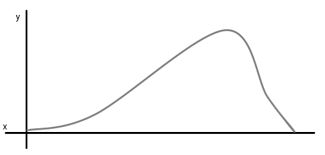
\includegraphics[width=0.2\textwidth]{img/neg_skew.png}
\end{center}

\choice{Positive Skew}{Negative Skew}{No Skew}{Not detectable}{a}

\question \textbf{For a symmetrical distribution, what is the value of $\beta_1?$}
\choice{0}{1}{-1}{$\infty$}{a}

% Situation Set Starts
\textbf{Answer the next SIX questions based on the following information}

\begin{center}
   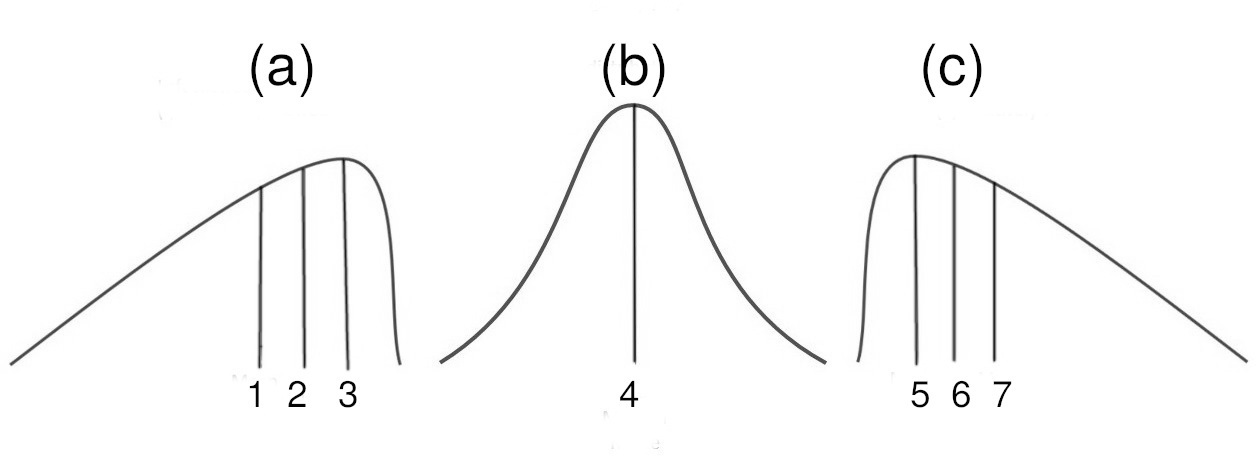
\includegraphics[width=0.5\textwidth]{../slide/img/skewness_clean.jpg}
\end{center}

\question \textbf{The curve (a) is an example of}
\choice{Positive Skew}{Negative Skew}{No Skew}{Not detectable}{b}

\question \textbf{The curve (b) is an example of}
\choice{Positive Skew}{Negative Skew}{No Skew}{Not detectable}{a}

\question \textbf{In Image (b), what is denoted by 4th value?}
\choice{Mean}{Median}{Mode}{All of the above}{d}

\question \textbf{In Image (c), what is in 6th value?}
\choice{Mean}{Median}{Mode}{None of the above}{b}

\question \textbf{What is the value corresponding to the position 3?}
\choice{Mean}{Median}{Mode}{None of the above}{c}

\question \textbf{What is the value corresponding to the position 7?}
\choice{Mean}{Median}{Mode}{None of the above}{a}
% Situation Set Ends

\question \textbf{If $\gamma_1 > 0$, the data is -}
\choice{Negatively skewed}{Positively skewed}{Symmetric}{Uncertain}{b}

\question \textbf{Which relationship is correct?}
\choice{$M_o = 2Me - \bar x$}{$M_o = 3Me - \bar x$}{$M_o = 3Me - 2 \bar x$}{$M_o = 2Me - 3 \bar x$}{c}

% Multiple Completion Starts
% TODO: incomplete question -- missing "Which one is correct?" prompt and \choice line
\question \textbf{Characteristics of a skewed distributon are --}

i. $Mean \ne Median \ne Mode$ \\
ii. Differences of upper and lower quartiles from median are unequal\\
iii. Frequency curve is asymmetric
% Multiple Completion Ends

\question \textbf{In a distribution, $\mu_2=25, \mu_3=20$, and $\mu_4=2200$; 
the distribution is --}
\choice{Negativelky skewed}{leptokurtic}{Platykurtic}{Symmetric}{b}

\question \textbf{For a data, $Q_3=41.6, Q_1=17.2, Median = 29, \& AM = 30$; What is Coefficient of skewness?}
\choice{24.4}{1}{0.03}{29.45}{d}

\question \textbf{In case of positive skewness, which one is correct?}
\choice{$Mean>Median>Mode$}{$Mean<Median<Mode$}{$Mean=Median=Mode$}
{$Mean>Median<Mode$}{a}

\question \textbf{For a symmetrical distribution, $\beta_1=$\textemdash}
\choice{1}{-1}{0}{3}{c}

\question \textbf{$\sqrt{\beta_1}=-0.23$ implies--}
\choice{Left Skew}{Symmetry}{Right Skew}{Mesokurtic}{a}

\question \textbf{$\gamma_1=0.43$ implies--}
\choice{Left Skew}{Symmetry}{Right Skew}{Mesokurtic}{c}

\question \textbf{$\gamma_1=0.0001$ implies--}
\choice{Left Skew}{Symmetry}{Right Skew}{Mesokurtic}{b}

\question \textbf{First 3 moments about 2 are 1, 2 and 8, respectively. 
What is the arithmetic mena?}
\choice{1}{2}{3}{4}{c}

\question \textbf{What is the second central moments of first 10 natural numbers?}
\choice{9.90}{9.09}{8.25}{5.67}{c}

\question \textbf{Frequencies of low and high values are smaller in -- distribution}
\choice{Positively skewed}{Negatively skewed}{Symmetric}{Mesokurtic}{c}

\question \textbf{Frequencies of higher values are smaller and of low values are
higher in -- distribution}
\choice{Positively skewed}{Negatively skewed}{Symmetric}{Mesokurtic}{a}

\question \textbf{Frequencies of higher values are higher and of low values are
lower in -- distribution}
\choice{Positively skewed}{Negatively skewed}{Symmetric}{Mesokurtic}{b}

% Multiple Completion Starts
\question \textbf{In a postively-skewed distribution--}

i. Frequencies of higher values are lower \\
ii. Frequencies of low values are higher \\
iii. Frequencies of higher values are higher

\textbf{Which one is correct?}

\choice{i and ii}{i and iii}{ii and iii}{i, ii and iii}{a}
% Multiple Completion Ends

% Multiple Completion Starts
\question \textbf{In a negatively-skewed distribution--}

i. Frequencies of higher values are lower \\
ii. Frequencies of low values are lower \\
iii. Frequencies of higher values are higher

\textbf{Which one is correct?}

\choice{i and ii}{i and iii}{ii and iii}{i, ii and iii}{c}
% Multiple Completion Ends

% Multiple Completion Starts
\question \textbf{In a symmetric distribution--}

i. Frequencies of higher values are lower \\
ii. Frequencies of low values are higher \\
iii. Frequencies of low values are lower 

\textbf{Which one is correct?}

\choice{i and ii}{i and iii}{ii and iii}{i, ii and iii}{b}
% Multiple Completion Ends

\question \textbf{Which formula is correct for determining skewness?}
\choice{$\gamma_1 = \sqrt{\frac{\mu_3^2}{\mu_2^3}}$}{$\gamma_1=\sqrt{\beta_1^2}$}{$\gamma_1 = \sqrt{\frac{\mu_3}{\mu_2^3}}$}{$\frac{\mu_2}{\sqrt{\mu_3^2}}$}{a}

\subsubsection{Situation Set}

% Situation Set Starts
\textbf{Answer the next THREE questions based on the following information}

\begin{center}
The arithmetic mean, Pearson's coefficient of skewness, and coefficient of variation of a distribution are 50, -0.4, and 40 \%, respectively. 
\end{center}

\question \textbf{What is the standard deviation?}
\choice{50}{20}{30}{40}{b}

\question \textbf{The Mode is --}
\choice{45}{50}{60}{58}{d}

\question \textbf{The Median is}
\choice{52.67}{5}{20}{10.39}{a}
% Situation Set Ends

% Situation Set Starts
\textbf{Answer the next two questions based on the following information}

\begin{center}
The first and second moments of a distribution around 2 are 13 and 195, respectively.
\end{center}

\question \textbf{What is the arithmetic mean?}
\choice{15}{12}{11}{26}{a}

\question \textbf{What is its variance?}
\choice{20}{21}{26}{25}{c}
% Situation Set Ends

\subsubsection{Multiple Completion}

% Multiple Completion Starts
\question \textbf{In a negatively skewed distribution --}

i. there is a long tail on the left \\
ii. median is greater than mean \\
iii. high values have frquencies  

\textbf{Which one is correct?}

\choice{i and ii}{i and iii}{ii and iii}{i, ii and iii}{d}
% Multiple Completion Ends

\subsection{Kurtosis}

\question \textbf{Which curve is platykurtic?}

\begin{center}
   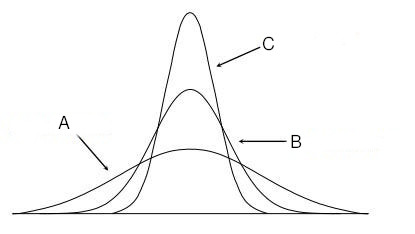
\includegraphics[width=0.4\textwidth]{img/kurtosis.jpg}
\end{center}

\choice{A}{B}{C}{None}{a}

\question \textbf{How many types of kurtosis are there?}
\choice{2}{3}{4}{5}{b}

\question \textbf{The standard deviation of a mesokurtik distribution is 2. What is the value of the 4th central moment?}
\choice{4}{8}{16}{48}{d}

\question \textbf{$\beta_2 = \sqrt 9$ implies data are--}
\choice{Leptokurtic}{Platykurtic}{Mesokurtic}{Symmetric}{c}

\question \textbf{$\beta_2 = 4$ implies data are--}
\choice{Leptokurtic}{Platykurtic}{Mesokurtic}{Symmetric}{a}

\question \textbf{$\beta_2 = 3$ implies data are--}
\choice{Leptokurtic}{Platykurtic}{Mesokurtic}{Symmetric}{c}

\question \textbf{$\beta_2 = 1$ implies data are--}
\choice{Leptokurtic}{Platykurtic}{Mesokurtic}{Symmetric}{b}

\question \textbf {The relationship between \( \beta_2 \) and \( \gamma_2 \) is --}
\choice{\( \beta_2 = \gamma_2 - 3 \)}{\( \gamma_2 = \beta_2 - 3 \)}{\( \gamma_2 = 3 \beta_2 \)}{\( \gamma_2 = \frac{\beta_2}{3} \)}{b}

\question \textbf{For a mesokurtik distribution, $\beta_2 = -$}
\choice{0}{-3}{3}{1}{c}

\question \textbf{What is the relationship between $\gamma_2$ and $\beta_2$?}
\choice{$\gamma_2 = \beta_2 + 3$}{$\gamma_2 = 2\beta_2 - 3$}{$\gamma_2 = \beta_2 - 1$}{$\gamma_2 = \beta_2 - 3$}{d}

\subsection{Misc}

\question \textbf{What is formula of the left inner fence for a box and whisker plot?}
\choice{$Q_1-1.5 \times IQR$}{$Q_3+1.5 \times IQR$}{$Q_1-3 \times IQR$}{$Q_3+1.5 \times IQR$}{a}

\question \textbf{What is the formula of IQR?}
\choice{$IQR = Q_3 + Q_1$}{$IQR = Q_3 - Q_1$}{$IQR = 2Q_3 - Q_1$}{$IQR = \frac{Q_3 - Q_1}{2}$}{b}

\question \textbf{Which is not used in constructing Box \& Whisker Plot?}
\choice{Mode}{$X_L$}{$Q_1 \& Q_3$}{$Q_1, Q_2 \& Q_3$}{a}

% Multiple Completion Starts
\question \textbf{In a symmatric distribution--}

i. Arithmetic Mean = Mode = Median \\
ii. $Q_2-Q_1 = Q_3-Q_2$  \\
iii. $Q_1-X_L = X_H-Q_3$

Which one is true?

\choice{i \& ii}{ii \& iii}{i \&iii}{i, ii \&iii}{d}
% Multiple Completion Ends

\subsection{Box and Whisker Plot}

\question \textbf{The following values represent the quartiles of a data set:}
\begin{itemize}
  \item Q1 = 25
  \item Q2 = 50
  \item Q3 = 75
\end{itemize}

\textbf{What is the interquartile range (IQR)?}
\choice{25}{50}{75}{100}{b}

% Multiple Completion Starts
\question \textbf{In a box and whisker plot, the following statements hold true:}

i. The length of the box represents the interquartile range (IQR). \\
ii. The whiskers extend from the minimum to the maximum data values. \\
iii. The median is represented by the top of the box.

\textbf{Which one is correct?}

\choice{i and ii}{i and iii}{ii and iii}{i, ii and iii}{a}
% Multiple Completion Ends

\subsection{Five Number Summary}

% Multiple Completion Starts
\question \textbf{In a given data set, the following values are recorded:}

i. The interquartile range is the difference between Q3 and Q1. \\
ii. The median is always equal to the mean. \\
iii. The maximum value in the five-number summary is the largest data point.

\textbf{Which one is correct?}

\choice{i and ii}{i and iii}{ii and iii}{i, ii and iii}{b}
% Multiple Completion Ends

% Multiple Completion Starts
\question \textbf{The five-number summary of a data set consists of the following:}

i. Minimum value \\
ii. Maximum value \\
iii. Median (Q2), First Quartile (Q1), Third Quartile (Q3)

\textbf{Which one is correct?}

\choice{i and ii}{i and iii}{ii and iii}{i, ii and iii}{d}
% Multiple Completion Ends

\question \textbf{Which is not included in five number summary?}
\choice{Arithmetic Mean}{$X_H$}{$Q_2$}{$Q_3$}{a}

\subsection{Situation Set}

% Situation Set Starts
\textbf{Answer the next THREE questions based on the following information}

For a frequency distribution, the following central moments are given:
\[
\mu_2 = 4, \quad \mu_3 = -4, \quad \mu_4 = 48
\]

\question \textbf{What is the variance of the distribution?}
\choice{2}{4}{8}{16}{b}

\question \textbf{What is Karl Pearson's coefficient of skewness based on moments ($\sqrt{\beta_1}$)?}
\choice{$-1.0$}{$-0.5$}{$0.5$}{$1.0$}{b}

\question \textbf{What is the kurtosis ($\beta_2$) of the distribution?}
\choice{2.5}{3.0}{3.5}{4.0}{b}
% Situation Set Ends

%------------------------------------------------------------------------------
\section{Correlation and Regression}
%------------------------------------------------------------------------------

\subsection{Correlation}

\question \textbf{The correlation coefficient between two variables lies between:}
\choice{0 and 1}{-1 and 0}{-1 and +1}{$-\infty$ and $+\infty$}{c}

\question \textbf{The correlation coefficient is unaffected by:}
\choice{Change of origin only}{Change of scale only}{Both change of origin and scale}{Neither}{c}

\question \textbf{A correlation coefficient of -0.85 indicates:}
\choice{Weak positive correlation}{Strong positive correlation}{Weak negative correlation}{Strong negative correlation}{d}

\question \textbf{If the correlation coefficient between X and Y is 0.6, the correlation between 2X and 3Y is:}
\choice{0.6}{0.2}{1.8}{Cannot be determined}{a}

\question \textbf{Correlation coefficient is the geometric mean of:}
\choice{Two regression coefficients}{Two variances}{Two means}{Two standard deviations}{a}

\question \textbf{When all points lie exactly on a straight line with positive slope, the correlation coefficient is:}
\choice{1}{0}{-1}{Infinity}{a}

\question \textbf{If X and Y are independent, the correlation coefficient is:}
\choice{1}{-1}{0}{Depends on sample}{c}

\question \textbf{The rank correlation coefficient is used when:}
\choice{Data is continuous}{Variables are quantitative}{Data is in ranks or ordinal}{Sample size is large}{c}

\question \textbf{Given covariance = 15, SD of X = 5, SD of Y = 4, the correlation coefficient is:}
\choice{0.60}{0.75}{0.80}{1.20}{b}

\question \textbf{The value of Spearman's rank correlation ranges between:}
\choice{-1 and +1}{0 and 1}{-1 and 0}{$-\infty$ and $+\infty$}{a}

\question \textbf{If the regression coefficients are 0.8 and 0.5, the correlation coefficient is:}
\choice{0.40}{0.63}{0.80}{1.30}{b}

\question \textbf{If the correlation coefficient is zero, the variables are:}
\choice{Perfectly positively correlated}{Perfectly negatively correlated}{Uncorrelated}{Highly correlated}{c}

\question \textbf{Who proposed the formula of correlation coefficient?}
\choice{R. A. Fisher}{Bowley}{Spearman}{Karl Pearson}{d} 

\question \textbf{Which of the following has the strongest correlation?}
\choice{-0.92}{0.67}{0.50}{0.91}{a}

\question \textbf{The lowest possible value of the correlation coefficient ---}
\choice{1}{0}{$-\infty$}{-1}{d}

\question \textbf{The linear association between two random variables is called --}
\choice{Correlation}{Regression}{Randomness}{Regularity}{a}

\question \textbf{Which measures the strength of inear association between two random variables?}
\choice{Correlation}{Regression}{Correlation coefficient}{Regression coefficient}{c}

\question \textbf{Karl Pearson's method of determining the strength of correlation is not applicable for ---}
\choice{Qualitative variable}{Quantitative variable}{Discrete variable}{Continuous variable}{a}

\question \textbf{For two independent variables, the value of the correlation coefficient is ---}
\choice{-1}{1}{$\infty$}{0}{d}

\question \textbf{Two variables having changes in same direction at same rates display ---}
\choice{Perfect negative correlation}{Partial positive correlation}{Perfect positive correlation}{Partial negative correlation}{c}

\question \textbf{Two variables having changes in opposite direction at same rates display ---}
\choice{Perfect negative correlation}{Partial positive correlation}{Perfect positive correlation}{Partial negative correlation}{a}

\question \textbf{Two variables having changes in same direction at different rates display ---}
\choice{Perfect negative correlation}{Partial positive correlation}{Perfect positive correlation}{Partial negative correlation}{b}

\question \textbf{Two variables having changes in opposite direction at different rates display ---}
\choice{Perfect negative correlation}{Partial positive correlation}{Perfect positive correlation}{Partial negative correlation}{d}

\question \textbf{When a variable is changing, but another is not affected, it is called}
\choice{Perfect negative correlation}{Partial positive correlation}{Perfect positive correlation}{Zero correlation}{d}

\question \textbf{TEXT }
\choice{Choice}{Choice}{Choice}{Choice}{a}

\question \textbf{Which of the following coefficients indicates strong negative correlation?}
\choice{-0.5}{-2}{0.67}{-0.94}{d}

\question \textbf{Which of the following has the strongest correlation?}
\choice{-0.5}{-2}{0.67}{-0.94}{d}

\question \textbf{If $b_1 = 0.25$ and $b_2 = -0.43$, which implies higher impact of the independent variable?}
\choice{$b_1$}{$b_2$}{Cannot be determined}{Equal impact}{c}

\subsection{Situation Set}

% Situation Set Starts
\textbf{Answer the next two questions based on the following information}

\begin{center}
A study was conducted to find the impact of study hour on students' GPA and the following was found:

$\displaystyle \sum (x_i- \bar x)(y_i - \bar y) = 30, \sum(x_i-\bar x)^2 = 45, \text{ and } \sum(y_i-\bar y)^2 = 55$
\end{center}

\question \textbf{What is the value of correlation coefficient?}
\choice{0.50}{0.60}{-0.60}{-0.50}{b}

\question \textbf{What is the value of $b_{yx}?$}
\choice{0.58}{-0.67}{0.67}{-1.75}{c}
% Situation Set Ends

\subsection{Multiple Completion}

% Multiple Completion Starts
\question \textbf{Which of the following are true about correlation?}

i. It measures the strength of linear relationship \\
ii. It is unitless \\
iii. Correlation implies causation

\textbf{Which one is correct?}

\choice{i and ii}{i and iii}{ii and iii}{i, ii and iii}{a}
% Multiple Completion Ends

%------------------------------------------------------------------------------
\section{Time Series}
%------------------------------------------------------------------------------

\question \textbf{Which is not a time series data?}
\choice{Number of calls received per week}{No. of road accidents on 
different days}{No. of earthquakes in different regions}
{No. of particles decayed in each second}{c}

\question \textbf{Which is not a time series data?}
\choice{Daily closing prices of a stock}{Annual temperature records of a city}
{Number of students in a each class}
{Number of visitors to a website each day}{c}

\question \textbf{Which is an example of time series data?}
\choice{Number of calls received by a call center each month}
{Height of children at different ages}
{Tota salary of all employees at a company}
{Population of different countries in 2020}{a}

% Multiple Completion Starts
\question \textbf{Which is a type of trend?}

i. Linear trend \\
ii. Non-linear trend \\
iii. Cyclic trend

\textbf{Which one is correct?}

\choice{i and ii}{i and iii}{ii and iii}{i, ii and iii}{a}
% Multiple Completion Ends

\question \textbf{Which can measure trend most precisely?}
\choice{Graphical method}{Semi-average method}{Moving average method}
{Quarter-average method}{c}

\question \textbf{Which is the multiplicative time series model?}
\choice{$Y_t = T_t \times S_t \times C_t \times R_t$}
{$Y_t = T_t \times D_t \times C_t \times R_t$}
{$Y_t = T_t \times P_t \times C_t \times R_t$}
{$Y_t = T_t \times G_t \times C_t \times R_t$}{a}

\question \textbf{In additive model, in the long run, $\sum R_t = --$}
\choice{0}{1}{Undefine}{Infinity}{a}

\question \textbf{In multiplicative time series model, in the long run, $\sum R_t = --$}
\choice{0}{1}{Undefined}{Infinity}{b}

% Situation Set Starts
\textbf{Answer the next two questions based on the following information}

Commodity wise export shipments (In million US\$) of Frozen and live 
fish in Bangladesh are given below. 

\begin{table}[h]
\centering
\begin{tabular}{c|c|c|c}
Months & 2022-23 (July-Dec) & 2023-24 (Jan-Jun) & 2022-23 (July-Dec) \\ \hline
Amount & 246.38 & 175.19 & 215.13
\end{tabular}
\caption{\label{usdrate}Source:\href{https://www.bb.org.bd/econdata/bop/exp_rcpt_merchandise.php}{BB} }
\end{table}

\question \textbf{Which component of time series is most evident?}
\choice{Irregular variation}{Cyclic variation}{Trend}{Seasonal variation}{d}

\question \textbf{Which value is most probable in the next period?}
\choice{200}{190}{130}{220}{b}
% Situation Set Ends

\question \textbf{A linear trend goes along a -- }
\choice{a curved line}{a wave}{straight line}{circle}{a}

\question \textbf{Which of the following is an example of seasonal variation in a time series?}  
\choice{Increase in ice cream sales during summer}{Rising fuel prices over decades}{Stock market crash}{Unemployment rate changes due to war}{a}  

\question \textbf{Which business is most likely to experience strong seasonal variation in its sales?}  
\choice{A supermarket}{A toy store}{A furniture store}{A gas station}{b}  

\question \textbf{Which of the following is an example of cyclic variation in a time series?}  
\choice{Boom and recession phases in an economy}{Increase in electricity consumption during summer}{High demand for umbrellas during the rainy season}{Sudden decline in stock prices due to a pandemic}{a}  

\question \textbf{Which of the following is an example of a trend in a time series?}  
\choice{Gradual increase in global average temperature}{Increase in ice cream sales during summer}{Fluctuations in stock prices due to news events}{Sudden drop in airline bookings due to a storm}{a}  

\question \textbf{Which type of trend is usually observed in a country's population growth over several decades?}  
\choice{Upward trend}{Downward trend}{Seasonal trend}{Cyclic trend}{a}  

\question \textbf{Which of the following best represents a downward trend in a time series?}  
\choice{Declining birth rates in a country over several decades}{Increase in online shopping during holiday seasons}{Fluctuations in stock market prices}{Sudden rise in fuel prices due to a crisis}{a}  

\question \textbf{Which factor is most likely to contribute to an upward trend in a company's annual revenue?}  
\choice{Improved marketing strategies over time}{Seasonal discounts and promotions}{Short-term fluctuations in customer demand}{Unpredictable supply chain disruptions}{a}  

\question \textbf{Which factor is most likely to cause cyclic variation in a time series?}  
\choice{Festive shopping trends}{Long-term business cycles}{Daily fluctuations in temperature}{Random fluctuations in demand}{b}  

\question \textbf{A non-linear trend goes along a --}
\choice{a curved line}{a wave}{a cubic pattern}{Any of the above}{d}

\question \textbf{Which measure of trend is subjective?}
\choice{Semi-average method}{Graphical method}{Moving average method}
{None of the above}{b}

% Situation Set Starts
\textbf{Answer the next THREE questions based on the following information}

\begin{table}[h]
\begin{tabular}{c|cccccccc}
Year & 2016 & 2017 & 2018 & 2019 & 2020 & 2021 & 2022 & 2023 \\ \hline
USD Exchange Rate & 78.35 & 79.49 & 82.87 & 83.26 & 84.60 & 84.37 & 85.80 & 106.70
\end{tabular}
\caption{\label{usdrate}Source--Investing.com}
\end{table}

\question \textbf{What is the second value of semi-average method?}
\choice{85.40}{90.37}{91.73}{89.78}{b}

\question \textbf{What kind of a trend do the data have?}
\choice{Upward}{Downward}{Both upward \& downward}{No trend}{a}

\question \textbf{Which component of time series is visible in the later 
part of the data?}
\choice{Seasonal Variation}{General Trend}{Irregular Variation}
{Cyclic Variation}{c}
% Situation Set Ends

% Situation Set Starts
\textbf{Answer the next THREE questions based on the following information}

\begin{table}[h]
\begin{tabular}{c|cccccccc}
Year & 2015 & 2016 & 2017 & 2018 & 2019 & 2020 & 2021 & 2022 \\ \hline
Average Temperature (°C) & 22.5 & 23.0 & 24.2 & 24.5 & 25.0 & 25.5 & 26.0 & 27.0
\end{tabular}
\caption{\label{tempdata}Source--National Weather Service}
\end{table}

\question \textbf{What is the second value of the semi-average method?}
\choice{25.75}{26.00}{25.88}{24.29}{c}

\question \textbf{What kind of trend do the data show?}
\choice{Upward}{Downward}{Both upward \& downward}{No trend}{a}

\question \textbf{Which component of the time series is most prominent in the data?}
\choice{Seasonal Variation}{General Trend}{Irregular Variation}{Cyclic Variation}{b}
% Situation Set Ends

% Situation Set Starts
\textbf{Answer the next THREE questions based on the following information}

\begin{table}[h]
\begin{tabular}{c|cccccccc}
Year & 2016 & 2017 & 2018 & 2019 & 2020 & 2021 & 2022 & 2023 \\ \hline
USD Exchange Rate & 78.35 & 79.49 & 82.87 & 83.26 & 84.60 & 84.37 & 85.80 & 106.70
\end{tabular}
\caption{\label{usdrate}Source--Investing.com}
\end{table}

\question \textbf{What is the second value of semi-average method?}
\choice{85.40}{90.37}{91.73}{89.78}{b}

\question \textbf{What kind of a trend do the data have?}
\choice{Upward}{Downward}{Both upward \& downward}{No trend}{a}

\question \textbf{Which component of time series is visible in the 
later part of the data?}
\choice{Seasonal Variation}{General Trend}{Irregular Variation}
{Cyclic Variation}{c}
% Situation Set Ends

% Situation Set Starts
\textbf{Answer the next THREE questions based on the following information}

\begin{table}[h]
\centering
\begin{tabular}{c|cccccccc}
Month & January & February & March & April & May & June & July & August \\ \hline
Rainfall (mm) & 150 & 120 & 180 & 200 & 160 & 140 & 170 & 190
\end{tabular}
\caption{\label{rainfalldata}Source: Meteorological Department}
\end{table}

\question \textbf{What is the semi-average for the second period of the data?}
\choice{160}{165}{180}{190}{b}

\question \textbf{Which type of trend do these rainfall data indicate?}
\choice{Increasing}{Decreasing}{No trend}{Fluctuating}{d}

\question \textbf{What is the primary variation component observed in the data?}
\choice{Seasonal Variation}{Trend Variation}{Cyclic Variation}
{Irregular Variation}{a}
% Situation Set Ends

\question \textbf{Time Series has how many components?}
\choice{2}{3}{4}{5}{c}

\question \textbf{Which component involves period more than one (01) year?}
\choice{Seasonal Variation}{Cyclic Variation}{Irregular Variation}{Random Variation}{b}

\question \textbf{Which one is not a component of Time Series}
\choice{Seasonal Variation}{Cyclic Variation}{General Trend}{Regular Variation}{d}

\question \textbf{A company is constantly getting greater revenue than previous year; this is--}
\choice{Seasonal Variation}{General Trend}{Irregular Variation}{Cyclic Variation}{b}

\question \textbf{Which is not a method of finding general trend?}
\choice{Graphical Method}{Moving Average}{Semi-Average}{Moving Median}{d}

% Situation Set Starts
\textbf{Answer the next two questions based on the following table:}

  \begin{table}[h]
\centering
\begin{tabular}{ccccccc}
Year     & 2007 & 2008 & 2009 & 2010 & 2011 & 2012\\ \hline
Sales & 5   & 35    & 34     & 40     & 42  & 204 
\end{tabular}
\end{table}

\question \textbf{In Semi-Average method, what is the 2nd average?}
\choice{74}{24.67}{95.33}{28}{c}

\question \textbf{What is the last  value of 3-yearly moving average?}
\choice{93.55}{95.53}{95.33}{59.33}{c}
% Situation Set Ends

\question \textbf{Which component of time series is affected by economic 
changes due to war?}
\choice{Trend}{Seasonal Variation}{Irregular Variation}{Cyclic Variation}{c}

\question \textbf{Which component of a time series captures long-term upward or downward movement?}  
\choice{Trend}{Seasonal Variation}{Irregular Variation}{Cyclic Variation}{a}  

\question \textbf{Which time series component represents fluctuations occurring at regular intervals within a year?}  
\choice{Trend}{Seasonal Variation}{Irregular Variation}{Cyclic Variation}{b}  

\question \textbf{Which component of time series is affected by economic 
changes during a recession?}
\choice{Trend}{Seasonal Variation}{Irregular Variation}{Cyclic Variation}{c}

\question \textbf{Which component of time series is most likely to be 
impacted by weather conditions like a monsoon season?}
\choice{Trend}{Seasonal Variation}{Irregular Variation}{Cyclic Variation}{b}

\question \textbf{Which component of time series would be influenced by 
government policy changes such as tax reforms?}
\choice{Trend}{Seasonal Variation}{Irregular Variation}{Cyclic Variation}{d}

% Situation Set Starts
\textbf{Answer the next three questions based on the following table:}

\begin{table}[h]
\centering
\begin{tabular}{ccccccc}
Year     & 2016 & 2017 & 2018 & 2019 & 2020 \\ \hline
Car Sales & 1200 & 1500 & 1700 & 1600 & 1800   
\end{tabular}
\end{table}

\question \textbf{What is the first value of the 2-yearly moving average?}
\choice{1350}{1300}{1400}{1250}{a}

\question \textbf{What is the last value of the 3-yearly moving average?}
\choice{1600}{1670}{1630}{1750}{c}

\question \textbf{What is the semi-average for the first period of the data?}
\choice{1350}{1400}{1450}{1300}{a}
% Situation Set Ends

\question \textbf{Demand for warm clothes is higher in winter season ans
less in summer. Which component of time series deals with this change?}
\choice{Trend}{Seasonal Variation}{Irregular Variation}{Cyclic Variation}{b}

\question \textbf{Death rates of a country for 7 years are given below:}

\begin{table}[H]
\centering
\begin{tabular}{c|c|c|c|c|c|c|l}
Year & 2009 & 2010 & 2011 & 2012 & 2013 & 2014 & 2015 \\ \hline
Rate & 5    & 7    & 6    & 8    & 7    & 12   & 13  
\end{tabular}
\end{table}

\textbf{In semi-average method, which year will be excluded?}
\choice{2012}{2013}{ 2015}{2009}{b}

\question \textbf{Which component of time series represents a natural disaster?}
\choice{Seasonal Variation}{General Trend}{Irregular Variation}{Cyclic Variation}{c}

\question \textbf{How many models of time series are there to combine the components?}
\choice{2}{3}{4}{5}{a}

\question \textbf{Which one reflects an irregular variation?}
\choice{Fluctuation in production due to war}{Price hike due to famine}{Rise of Temperature to drought}{Any of the above}{d}

\subsection{Situation Set}

% Situation Set Starts
\textbf{Answer the next three questions based on the following table:}

\question \textbf{Death rates of a country for 7 years are given below:}

\begin{table}[H]
\centering
\begin{tabular}{c|c|c|c|c|c|c|l}
Year & 2009 & 2010 & 2011 & 2012 & 2013 & 2014 & 2015 \\ \hline
Rate & 5    & 7    & 6    & 8    & 7    & 12   & 13  
\end{tabular}
\end{table}

\textbf{In semi-average method, what is the first average?}
\choice{5}{7}{6}{8}{c}

\question \textbf{What is the first value of the 2-yearly moving average?}
\choice{5}{6}{7}{8}{b}

\question \textbf{What is the last value of the 3-yearly moving average?}
\choice{11.10}{9.68}{10.65}{10.67}{c}
% Situation Set Ends

% Situation Set Starts
\textbf{Answer the next three questions based on the following table:}

\textbf{The following table shows the population growth rate (in percentage) of a city over seven years.}

\begin{table}[H]
\centering
\begin{tabular}{c|c|c|c|c|c|c|c}
Year  & 2015 & 2016 & 2017 & 2018 & 2019 & 2020 & 2021 \\ \hline
Rate (\%) & 2.5  & 2.7  & 3.1  & 3.6  & 3.9  & 4.2  & 4.5  
\end{tabular}
\end{table}

\question \textbf{What is the average population growth rate over the 7 years?}
\choice{3.2\%}{3.5\%}{3.6\%}{3.8\%}{b}

\question \textbf{What is the second value in the 3-yearly moving average?}
\choice{2.8\%}{3.1\%}{3.3\%}{3.5\%}{b}

\question \textbf{Using the semi-average method, what is the second average?}
\choice{3.6\%}{3.7\%}{3.8\%}{4.0\%}{c}
% Situation Set Ends

% Situation Set Starts
\textbf{Answer the next three questions based on the following table:}

\textbf{The following table shows the annual rainfall (in cm) recorded in a region over seven years.}

\begin{table}[H]
\centering
\begin{tabular}{c|c|c|c|c|c|c|c}
Year   & 2010  & 2011  & 2012  & 2013  & 2014  & 2015  & 2016  \\ \hline
Rainfall (cm) & 85   & 90   & 88   & 92   & 95   & 100  & 105  
\end{tabular}
\end{table}

\question \textbf{What is the median annual rainfall for the given years?}
\choice{90 cm}{92 cm}{93 cm}{95 cm}{b}

\question \textbf{What is the first value of the 2-yearly moving average?}
\choice{86.5 cm}{87 cm}{88.5 cm}{89 cm}{a}

\question \textbf{Using the semi-average method, what is the first average?}
\choice{88 cm}{89 cm}{90 cm}{91 cm}{b}
% Situation Set Ends

% Situation Set Starts
\textbf{Answer the next three questions based on the following table:}

\textbf{The following table shows the average monthly temperature (in °C) recorded in a city over seven months.}

\begin{table}[H]
\centering
\begin{tabular}{c|c|c|c|c|c|c|c}
Month  & Jan & Feb & Mar & Apr & May & Jun & Jul \\ \hline
Temperature (°C) & 12  & 14  & 18  & 22  & 26  & 30  & 32  
\end{tabular}
\end{table}

\question \textbf{What is the mean temperature over the given months?}
\choice{19.5°C}{20.5°C}{21.5°C}{22.5°C}{c}

\question \textbf{What is the third value in the 3-monthly moving average?}
\choice{16°C}{18°C}{20°C}{22°C}{b}

\question \textbf{Using the semi-average method, what is the second average temperature?}
\choice{24°C}{25°C}{26°C}{27°C}{c}
% Situation Set Ends

% Situation Set Starts
\textbf{Answer the next three questions based on the following table:}

\textbf{The following table shows the monthly sales revenue (in thousand dollars) of a store over seven months.}

\begin{table}[H]
\centering
\begin{tabular}{c|c|c|c|c|c|c|c}
Month  & Jan & Feb & Mar & Apr & May & Jun & Jul \\ \hline
Revenue (000\$) & 50  & 55  & 60  & 70  & 75  & 80  & 85  
\end{tabular}
\end{table}

\question \textbf{Which month had the highest sales revenue?}
\choice{May}{Jun}{Jul}{Apr}{c}

\question \textbf{What is the first value of the 2-monthly moving average?}
\choice{52.5}{55}{57.5}{60}{a}

\question \textbf{Using the semi-average method, what is the first average revenue?}
\choice{57.5}{55}{62.5}{65}{b}
% Situation Set Ends

\subsection{Multiple Completion}

% Multiple Completion Starts
\question \textbf{Which of the following are components of a time series?}

i. Trend \\
ii. Seasonal Variation \\
iii. Correlation

\textbf{Which one is correct?}

\choice{i and ii}{i and iii}{ii and iii}{i, ii and iii}{a}
% Multiple Completion Ends

% Multiple Completion Starts
\question \textbf{Which statements about time series models are correct?}

i. The additive model adds all the components \\
ii. The multiplicative model also contains some additions. \\
iii. Additive and multiplicative models produce identical forecasts.

\textbf{Which one is correct?}

\choice{ii}{iii}{i}{i, ii and iii}{c}
% Multiple Completion Ends

% Multiple Completion Starts
\question \textbf{Which of the following are methods of estimating trend in time series?}

i. Moving Average Method \\
ii. Sem-average method \\
iii. Simple Random Sampling

\textbf{Which one is correct?}

\choice{i and ii}{i and iii}{ii and iii}{i, ii and iii}{a}
% Multiple Completion Ends

%-------------------------------------------------------------------------------
\section{Published Statistics in Bangladesh}
%-------------------------------------------------------------------------------

% Multiple Completion Starts
\question \textbf{Limitations of published statistics in Bangladesh are --}

i. Wrong data collection method \\
ii. Insufficient data \\
iii. Lack of proper training

\textbf{Which one is correct?}

\choice{i and ii}{i and iii}{ii and iii}{i, ii and iii}{d}
% Multiple Completion Ends

\question \textbf{How many sources of published statistics are there in Bangladesh?}
\choice{2}{3}{4}{6}{b}

\question \textbf{Bangladesh Bureau of Statistics collect -- }
\choice{Official statistics}{Non-official statistics}{Semi-official statistics}{None of the above}{a}

\question \textbf{Which statistics are published by an NGO?}
\choice{Official statistics}{Non-official statistics}
{Semi-official statistics}{None of the above}{c}

\question \textbf{The primary source of official statistics in Bangladesh is --}
\choice{WHO}{BBS}{CPD}{UNDP}{b}

\question \textbf{Which statistics are typically published by NGOs like World Wildlife Fund (WWF)?}
\choice{Official statistics}{Non-official statistics}{Semi-official statistics}{None of the above}{b}

\question \textbf{Which organization typically publishes non-official statistics in the field of health?}
\choice{UNICEF}{World Health Organization (WHO)}{World Bank}{United Nations (UN)}{b}

\question \textbf{In Bangladesh, a census is usually done every -- years}
\choice{20}{15}{10}{12}{c}

\question \textbf{Population census is --}
\choice{Official statistics}{Non-official statistics}
{Semi-official statistics}{None of the above}{a}

\question \textbf{In Bangladesh, which ministry present the budget?}
\choice{Planning}{Education}{Finance}{Agriculture}{c}

%\question \textbf{To complete the song, the last answer should be
%\choice{a}{b}{c}{d}{e} % Invalid answer choice

\end{questions}

\newpage  %Uncomment to put on new age
\bigskip

\begin{multicols}{3}
[
Answer Key: 
]
\showallanswers % Phil Hirschorn
\end{multicols}
\global\setbox\allanswers=\vbox{}

% ============================== PAPER 2 ==============================
\clearpage
\setcounter{section}{0}
\renewcommand{\theHsection}{2.\arabic{section}}% unique link names per paper
\phantomsection
\addcontentsline{toc}{part}{Second Paper}
\begin{center}\Large\textbf{Statistics -- Second Paper}\end{center}

 \section{Introduction to Probability}

\begin{questions}

\subsection {Permutation-Combination}

\question \textbf{Three objects can be placed in 2 positions in -- ways.}
\choice{3}{4}{6}{8}{c}

\question \textbf{In how many ways can a team of 2 be formed from 4 people?}
\choice{4}{6}{8}{12}{b}

\question \textbf{$\displaystyle ^np_r=$}
\choice{$\displaystyle \frac {n!}{(n-r)!}$}{$\displaystyle \frac {n!}{(n+r)!}$}{$\displaystyle \frac {n!}{r!}$}{$\displaystyle \frac {n!}{(r-n)!}$}{a}

\question \textbf{$\displaystyle ^nC_r=$}
\choice{$\displaystyle \frac {n!}{(n-1)!(n+r)!}$}{$\displaystyle \frac {r!}{n!(n-r)!}$}{$\displaystyle \frac {n!(n-1)!}{r!}$}{$\displaystyle \frac {n!}{(r-n)!}$}{a}

%-----------------------------------------------------------------
\subsection {Conceptual Questions}
%-----------------------------------------------------------------

\question \textbf{What is the probability that at least one item in a sample space will occurr?}
\choice{0}{0.5}{1}{Undefined}{c}

\question \textbf{The probability of two disjoint sets happening together is:}
\choice{0.5}{0}{1}{$0  \leq x < 1$}{b}

\question \textbf{How many additive laws of probability are there?}
\choice{1}{2}{3}{4}{b}

\question \textbf{$P(A\cup B) = P(A) + P(B)$ implies A \& B are --}
\choice{Disjoint}{Independent}{Joint}{Independent}{a}

\question \textbf{$P(A\cap B) = P(A) \times P(B)$ implies A \& B are --}
\choice{Disjoint}{Independent}{Joint}{Independent}{b}

\question \textbf{Which is the formula of classical approach of probability?}
\choice{$P=\frac{\text{No. of favorable outcomes}}{\text{Total no. of possible outcomes}}$}{$P=\frac{\text{No. of total outcomes}}{\text{No. of favorable outcomes}}$}{$P = \lim_{n(S)\to\infty} \frac{n(A)}{n(S)}$}{$P = \lim_{n(A)\to\infty} \frac{n(A)}{n(S)}$}{a}

\question \textbf{Which is the formula of empirical/relative frequency approach of probability?}
\choice{$P=\frac{\text{No. of favorable outcomes}}{\text{Total no. of possible outcomes}}$}{$P=\frac{\text{No. of total outcomes}}{\text{No. of favorable outcomes}}$}{$\displaystyle P = \lim_{n(S)\to\infty} \frac{n(A)}{n(S)}$}{$\displaystyle P = \lim_{n(A)\to\infty} \frac{n(A)}{n(S)}$}{a}

\question \textbf{What is the correct formula for conditional probability?}
\choice{$P(A|B) = \frac{P(A \cap B)}{P(B|A)}$}{$P(A|B) = \frac{P(A \cap B)}{P(A)}$}{$P(A|B) = \frac{P(A \cap B)}{P(B)}$}{$P(A|B) = \frac{P(B|A)}{P(B|A)}$}{a}

\question \textbf{The third axiom of probability is --}
\choice{$0 \le P(A) \le 1$}{$P(S) = 1$}{$\displaystyle P(A_1 U A_2 U \cdots U
A_n) = \sum_{i=1}^{\infty}P(A_i)$}{$P(A) = 1 - P(A)$}{c}

% Multiple Completion Starts
\question \textbf{Possible value of probability}

i. -1 \quad
ii. 0.5 \quad
iii. 0

\textbf{Which one is correct?}

\choice{i and ii}{i and iii}{ii and iii}{i, ii and iii}{c}
% Multiple Completion Ends

\question \textbf{An act repeated under some specific conditions is called --}
\choice{Event}{Experiment}{Sample}{Sample space}{b}

\question \textbf{$P(0)$ implies -- }
\choice{A certain event}{An uncertain event}{An impossible event}{A probable event}{c}

\question \textbf{Events having some common elements are called --}
\choice{Complementary events}{Mutually exclusive events}{Exhaustive events}{Non-Mutually exclusive events events}{a}

\question \textbf{The minimum value of probability is}
\choice{$-\alpha$}{1}{0}{-1}{c}

\question \textbf{Each element of sample space is called--}
\choice{Trial}{Experiment}{Variable}{Sample Point}{d}

\question \textbf{Two events not ocurring together are called--}
\choice{dependent Events}{Independent Events}{Mutually Exclusive Events}{Marginal Events}{c}

\question \textbf{If A and B are independent, which formula is correct?}
\choice{$P(A \cap B) = P(A) \cdot P(B)$}{$P(A \cap B) = P(\bar A) \cdot P(B)$}{$P(A \cap B) = P(A) \cdot P(\bar B)$}{$P(A \cap \bar B) = P(A) \cdot P(B)$}{a}

\question \textbf{Which of the following are disjoint events?}
\choice{$A = \{1, 2, 3\}, B = \{4, 5\}$}{$A = \{a, b\}, B = \{b, c\}$}{$A = \{0\}, B = \{0, 1\}$}{$A = \{x, y\}, B = \{x, y\}$}{a}

\question \textbf{Which of the following are disjoint events?}
\choice{$P = \{1, 2\}, Q = \{2, 3\}$}{$P = \{x\}, Q = \{x, y\}$}{$P = \{1, 3\}, Q = \{3, 5\}$}{$P = \{m, n\}, Q = \{p, q\}$}{d}

% Multiple Completion Starts
\question \textbf{Let the sample space be $S = \{1, 2, 3, \dots, 10\}$. Which of the following pairs of events are disjoint?}

i. $A$: Number is prime, \quad $B$: Number is greater than 3 \\
ii. $A$: Number is even, \quad $B$: Number is divisible by 3 \\
iii. $A$: Number is less than 5, \quad $B$: Number is greater than 6

\textbf{Which one is correct?}

\choice{i and ii}{i and iii}{ii and iii}{i, ii and iii}{c}
% Multiple Completion Ends

% Multiple Completion Starts
\question \textbf{Let $S = \{1, 2, \dots, 10\}$. Which of the following event pairs are disjoint?}

i. $A$: Number is divisible by 2, \quad $B$: Number is divisible by 5 \\
ii. $A$: Number is less than 7, \quad $B$: Number is odd \\
iii. $A$: Number is a prime, \quad $B$: Number is a multiple of 4

\textbf{Which one is correct?}

\choice{i and iii}{i and ii}{ii and iii}{i, ii and iii}{a}
% Multiple Completion Ends

% Multiple Completion Starts
\question \textbf{Let the sample space be $S = \{1, 2, 3, \dots, 10\}$. Which of the following pairs of events are disjoint?}

i. $A$: Number is a multiple of 4, \quad $B$: Number is odd \\
ii. $A$: Number is less than 4, \quad $B$: Number is greater than 8 \\
iii. $A$: Number is a square, \quad $B$: Number is even

\textbf{Which one is correct?}

\choice{i and ii}{i and iii}{ii and iii}{i, ii and iii}{a}
% Multiple Completion Ends

\question \textbf{Let $S = \{1, 2, 3, \dots, 10\}$. Which of the following pairs of events are disjoint?}

\choice{$A$: Multiples of 3, $B$: Multiples of 5}{%
$A$: Prime numbers, $B$: Even numbers greater than 2}{%
$A$: Numbers less than 4, $B$: Numbers greater than 6}{%
All of the above}{d}

\subsection{Numbers}

\question \textbf{A number is randomly chosen from a list of 10 consecutive positive
integers. What is the probability that the number selected is greater than the
average (arithmetic mean) of all 10 integers?}
\choice{$\frac 13$}{$\frac 34$}{$\frac 4{10}$}{$\frac 12$}{d}

\question \textbf{10 out of each 100 people in a city walk to the office. If one is picked randomly, what is the probability s/he does not walk to the office?}
\choice{0.95}{0.10}{0.90}{0.01}{c}

\question \textbf{In a school, 15 out of 100 students prefer online classes over in-person classes. If a student is selected randomly, what is the probability that they prefer in-person classes?}  
\choice{0.15}{0.85}{0.75}{0.25}{b}  

\question \textbf{A factory reports that 8 out of every 100 manufactured items are defective. If an item is chosen at random, what is the probability that it is not defective?}  
\choice{0.08}{0.92}{0.80}{0.12}{b}  

\question \textbf{A hospital study finds that 12\% of patients do not prefer evening appointments. If a patient is selected at random, what is the probability that they prefer evening appointments?}  
\choice{0.12}{0.78}{0.88}{0.18}{c}  

\question \textbf{A survey shows that 5 out of every 200 customers in a store pay with cash. If a customer is picked randomly, what is the probability that they pay using another method?}  
\choice{0.050}{0.500}{0.975}{0.025}{c}  

%-----------------------------------------------------------------
\subsection {Coin-Die}
%-----------------------------------------------------------------

\question \textbf{Tossing a die r times generates how many outcomes?}
\choice{$6\times r$}{$r^6$}{$6^r$}{$2^r$}{c}

\question \textbf{Tossing a coin r times generates how many outcomes?}
\choice{$2\times r$}{$r^2$}{$2^r$}{$6^r$}{c}

\question \textbf{A coin is thrown thrice. How many outcomes are generated?}
\choice{3}{4}{8}{9}{c}

\question \textbf{A coin is thrown twice. What is the probability of getting 2 heads?}
\choice{$\frac14$}{$\frac13$}{$\frac12$}{$\frac24$}{a}

\question \textbf{A fair coin is tossed twice. What is the probability of getting at least one tail?}  
\choice{$\frac14$}{$\frac12$}{$\frac34$}{$\frac13$}{c}  

\question \textbf{Two fair coins are tossed simultaneously. What is the probability of getting exactly one head?}  
\choice{$\frac14$}{$\frac12$}{$\frac34$}{$\frac13$}{b}  

\question \textbf{A coin is flipped twice. What is the probability of getting heads first and tails second?}  
\choice{$\frac14$}{$\frac13$}{$\frac12$}{$\frac24$}{a}  

\question \textbf{If two fair coins are tossed together, what is the probability of getting at least one head?}  
\choice{$\frac12$}{$\frac13$}{$\frac34$}{$\frac14$}{c}  

\question \textbf{A fair coin is tossed twice. What is the probability of getting two tails?}  
\choice{$\frac12$}{$\frac13$}{$\frac14$}{$\frac24$}{c}  

\question \textbf{Two fair coins are tossed. What is the probability that at least one of them lands on tails?}  
\choice{$\frac34$}{$\frac12$}{$\frac14$}{$\frac13$}{a}  

\question \textbf{A die is thrown twice. This is called --}
\choice{An experiment}{sample space}{A random experiment}{A trial}{a}

\question \textbf{If a neutral die is thrown, the probability of having a digit greater than 6 is}
\choice{$\frac 1 6$}{$\frac 0 6$}{$\frac 2 3$}{$\frac 3 6$}{b}

\question \textbf{Tossing a coin twice generates how many outcomes?}
\choice{4}{16}{8}{2}{a}

\question \textbf{A die is rolled twice. How many possible outcomes are there?}
\choice{6}{12}{36}{18}{c}

%-----------------------------------------------------------------
\subsection {Balls-Cards}
%-----------------------------------------------------------------

\question \textbf{There are 3 red, 4 black, and 5 white balls in an urn. If two balls are randomly taken, what is the probability that both are red?}
\choice{$\frac{1}{66}$}{$\frac{1}{22}$}{$\frac{2}{22}$}{$\frac{3}{11}$}{b}

\question \textbf{There are 3 red, 4 black, and 5 white balls in an urn. If two balls are randomly taken, what is the probability that neither is red?}  
\choice{$\frac{5}{11}$}{$\frac{6}{11}$}{$\frac{3}{11}$}{$\frac{5}{22}$}{b}  

\question \textbf{A jar contains 6 blue and 4 green marbles. If two marbles are drawn at random, what is the probability that both are blue?}  
\choice{$\frac{5}{18}$}{$\frac{1}{3}$}{$\frac{1}{2}$}{$\frac{1}{4}$}{b}  

\question \textbf{A box has 7 black and 5 white balls. If one ball is drawn at random, what is the probability that it is not black?}  
\choice{$\frac{7}{12}$}{$\frac{5}{12}$}{$\frac{1}{2}$}{$\frac{1}{3}$}{b}  

\question \textbf{A bag contains 8 red and 6 white balls. If two balls are drawn at random, what is the probability that they are of different colors?}  
\choice{$\frac{24}{91}$}{$\frac{58}{91}$}{$\frac{48}{91}$}{$\frac{72}{91}$}{c}  

\question \textbf{A box contains 9 blue and 3 red balls. If two balls are randomly picked, what is the probability that at least one is red?}  
\choice{$\frac{3}{11}$}{$\frac{1}{3}$}{$\frac{18}{33}$}{$\frac{5}{11}$}{d}  

% Situation Set Starts
\textbf{Answer the next THREE questions based on the following information.}

A card is drawn from of pack of playing cards.

\question \textbf{What is the probability that the card is a King?}
\choice{0.0192}{0.25}{0.5}{0.0769}{d}

\question \textbf{P(The card is not from Diamonds)--}
\choice{$\frac12$}{$0$}{$\frac34$}{$\frac14$}{c}

\question \textbf{P(The card is red or Clubs)}
\choice{$\frac14$}{$\frac12$}{$\frac23$}{$\frac34$}{d}
% Situation Set Ends

% Situation Set Starts
\textbf{Answer the next THREE questions based on the following information.}

A card is drawn at random from a standard deck of 52 playing cards.

\question \textbf{What is the probability that the card is a Queen?}
\choice{0.0192}{0.0769}{0.25}{0.5}{b}

\question \textbf{P(The card is not a Spade)}  
\choice{$\frac14$}{$\frac12$}{$\frac34$}{$\frac13$}{c}

\question \textbf{P(The card is black or a Heart)}  
\choice{$\frac12$}{$\frac34$}{$\frac13$}{$\frac14$}{a}
% Situation Set Ends

% Situation Set Starts
\textbf{Answer the next TWO questions based on the following information.}

An urn contains 5 red, 7 blue, and 8 green balls.

\question \textbf{What is the probability that the ball drawn is red?}
\choice{0.26}{0.25}{0.2}{0.4}{a}

\question \textbf{P(The ball drawn is not blue)--}
\choice{$\frac{13}{20}$}{$0.5$}{$\frac{7}{20}$}{$\frac{8}{20}$}{a}
% Situation Set Ends

%-----------------------------------------------------------------
\subsection {Set-Problems}
%-----------------------------------------------------------------

\question \textbf{In a class of 40 students, 23 passed in Mathematics, 25 passed in English, and 10 failed in both the subjects. A student is randomly selected. What is the probability that the student passed in at least one subject}
\choice{$\frac13$}{$\frac14$}{$\frac34$}{$\frac45$}{c}

\question \textbf{In a survey of 60 people, 35 liked coffee, 28 liked tea, and 12 liked neither. If a person is selected at random, what is the probability that they like at least one of the two beverages?}
\choice{$\frac{3}{5}$}{$\frac{4}{5}$}{$\frac{2}{3}$}{$\frac{5}{6}$}{b}

% Situation Set Starts
\textbf{Answer the next two questions based on the following information}

\textbf{In a class of 40 students, 23 passed in Mathematics, 25 passed in English, and 10 failed in both the subjects. A student is randomly selected.}

\question What is the probability that the student passed in at least one subject?
\choice{$\frac13$}{$\frac14$}{$\frac34$}{$\frac45$}{c}

\question What is the probability that the student passed in passed in both the subjects?
\choice{$\frac{11}{20}$}{$\frac{9}{20}$}{$\frac{4}{5}$}{$\frac{19}{20}$}{b}
% Situation Set Ends

\question What is the probability that the student passed in passed in passed in Mathematics alone?
\choice{$\frac{1}{8}$}{$\frac{9}{20}$}{$\frac{3}{10}$}{$\frac{6}{13}$}{a}

\question \textbf{For two independent events $A$ and $B$, which one is correct?}
\choice{$P(A\cap B) = P(A) \times P(B)$}{$P(A\cup B) = P(A) + P(B)$}{$P(A\cap B) = P(A) - P(B)$}{$P(A\cup B) = P(A) \times P(B)$}{a}

\question \textbf{For two mutually exclusive events $A$ and $B$, which one is correct?}
\choice{$P(A\cap B) = P(A) \times P(B)$}{$P(A\cup B) = P(A) + P(B)$}{$P(A\cap B) = P(A) - P(B)$}{$P(A\cup B) = P(A) \times P(B)$}{b}

\question \textbf{Which of the following correct?}
\choice{$\displaystyle \frac{P(A)}{P(B)}= \frac{P(B|A)}{P(A|B)}$}{$\displaystyle \frac{P(A)}{P(A|B)}= \frac{P(B|A)}{P(B)}$}{$\displaystyle \frac{P(A)}{P(B)}= \frac{P(B|A)}{P(B)}$}{$\displaystyle \frac{P(A)}{P(B)}= \frac{P(A|B)}{P(B|A)}$}{d}

\question \textbf{The probability of rain is $\frac 16$ for any given day next week. What is the probability that it will rain on both Monday and Tuesday?}
\choice{$\frac 16$}{$\frac 1{36}$}{$\frac 56$}{$\frac 1{17}$}{b}

\question \textbf{Given \( P(A \cup B) = 0.7 \), \( P(A \cap B) = 0.2 \), what are \( P(A) \) and \( P(B) \)?}  
\choice{$P(A) = 0.5 \text{ and } P(B) = 0.4
$}{$P(A) = 0.4 \text{ and } P(B) = 0.6$}{$P(A) = 0.4 \text{ and } P(B) = 0.3$}{$P(A) = 0.7 \text{ and } P(B) = 0.3$}{a}

\question \textbf{If \( P(A) = 0.4 \), \( P(B) = 0.5 \), and \( P(A \cup B) = 0.7 \), what is \( P(A \cap B) \)?}  
\choice{$0.2$}{$0.1$}{$0.3$}{$0.4$}{a}

\question \textbf{Given \( P(A) = 0.3 \), \( P(A \cup B) = 0.6 \), and \( P(A \cap B) = 0.1 \), what is \( P(B) \)?}  
\choice{$0.6$}{$0.4$}{$0.3$}{$0.2$}{b}

\question \textbf{If \( P(A) = 0.5 \), \( P(B) = 0.6 \), and \( P(A \cap B) = 0.3 \), what is \( P(A \cup B) \)?}  
\choice{$0.8$}{$0.9$}{$0.7$}{$1$}{c}

\question \textbf{If \( P(A) = 0.2 \), \( P(B) = 0.3 \), and \( P(A \cup B) = 0.4 \), what is \( P(A \cap B) \)?}  
\choice{$0.9$}{$0.2$}{$0.3$}{$0.1$}{d}

\question \textbf{Given \( P(A) = 0.7 \), \( P(A \cup B) = 0.9 \), and \( P(A \cap B) = 0.5 \), what is \( P(B) \)?}  
\choice{$0.8$}{$0.6$}{$0.7$}{$0.5$}{c}

% Situation Set Starts
\textbf{Answer the next two questions based on the following information}

\begin{center}
For two exhaustive evenst A \& B, P(A) = 0.7 and P(B) = 0.4
\end{center}

\question \textbf{$P(A\cap B) = ?$}
\choice{0.1}{0.3}{0.6}{1}{a}

% Multiple Completion Starts
\question \textbf{The events A \& B are --}

i. independent \\
ii. dependent \\
iii. not mutually exclusive

\textbf{Which one is correct?}

\choice{i and ii}{i and iii}{ii and iii}{i, ii and iii}{c}
% Multiple Completion Ends
% Situation Set Ends

% Situation Set Starts
\textbf{Answer the next three questions using the following information}

$P(A) = \frac 1 3, P(B) = \frac 1 2 \space \& \space P(A\cup B) = \frac 7 {12}$

\question \textbf{$P(A \cap B) = ?$}
\choice{$\frac {5}{12}$}{$\frac12$}{$\frac{1}{4}$}{$\frac{15}{16}$}{c}

\question \textbf{$P(A \cap \bar B)=?$}
\choice{$\frac{1}{4}$}{$\frac{3}{4}$}{$\frac{5}{6}$}{$\frac{1}{12}$}{a}

\question \textbf{What is the probability that B occurs or A does not occur?}
\choice{$\frac{3}{4}$}{$\frac{7}{12}$}{$\frac{5}{12}$}{$\frac{11}{12}$}{d}
% Situation Set Ends

% Situation Set Starts
\textbf{Answer the next three questions using the following information}

$P(C) = \frac 2 5, P(D) = \frac 3 4 \space \& \space P(C \cup D) = \frac{9}{10}$

\question \textbf{$P(C \cap D) = ?$}
\choice{$\frac{1}{10}$}{$\frac{1}{4}$}{$\frac{7}{20}$}{$\frac{4}{5}$}{b}

\question \textbf{$P(C \cap \bar D)=?$}
\choice{$\frac{1}{10}$}{$\frac{2}{5}$}{$\frac{3}{20}$}{$\frac{3}{10}$}{c}

\question \textbf{What is the probability that D occurs or C does not occur?}
\choice{$\frac{17}{20}$}{$\frac{7}{10}$}{$\frac{3}{4}$}{$\frac{11}{20}$}{a}
% Situation Set Ends

% Situation Set Starts
\textbf{Answer the next three questions using the following information:}

$P(E) = \frac 1 3, P(F) = \frac 1 4 \space \& \space P(E \cap F) = \frac{1}{10}$

\question \textbf{$P(E \cup F) = ?$}
\choice{$\frac{1}{58}$}{$\frac{3}{10}$}{$\frac{58}{60}$}{$\frac{58}{120}$}{c}

\question \textbf{$P(E \cap \bar F)=?$}
\choice{$\frac{7}{40}$}{$\frac{7}{30}$}{$\frac{3}{10}$}{$\frac{1}{30}$}{b}

\question \textbf{What is the probability that F occurs or E does not occur?}
\choice{$\frac{11}{30}$}{$\frac{19}{30}$}{$\frac{13}{40}$}{$\frac{23}{30}$}{d}
% Situation Set Ends

\question \textbf{An un contains 10 red and 5 black balls. Two balls are drawn; what is the probability of getting two red balls?}
\choice{$\frac 37$}{$\frac 47$}{$\frac {20}{21}$}{$\frac 2{21}$}{a}

\subsection{Situation Set}

% Situation Set Starts
\textbf{Answer the next two questions based on the following information}

\begin{center}
For two comprehensive events $A$ and $B, P(A) = 0.8, \text{ and } P(B) = 0.6$; 
\end{center}
\question \textbf{What is the value of $P(A \cap B)?$}
\choice{0.1}{0.2}{0.3}{0.4}{d}

% Multiple Completion Starts
\question \textbf{The events $A$ and $B$ are --}

i. independent \\
ii. dependent \\
iii. non-disjoint

\textbf{Which one is correct?}

\choice{i and ii}{i and iii}{ii and iii}{i, ii and iii}{c}
% Multiple Completion Ends
% Situation Set Ends

\subsection{Multiple Completion}

% Multiple Completion Starts
\question \textbf{$P(A) = \frac23, P(B) = \frac15, \text{and} P(A \cap B) = \frac16$}

i. $A$ and $B$ are independent \\
ii. $P(A \cup B) = \frac{7}{10}$ \\
iii. $P(\bar A) = \frac 13$

\textbf{Which one is correct?}

\choice{i and ii}{i and iii}{ii and iii}{i, ii and iii}{c}
% Multiple Completion Ends

% Multiple Completion Starts
\question \textbf{$P(A) = 0$ implies}

i. $A$ is an impossible event \\
ii. $A$ would ocurr in extreme cases \\
iii. $P(\bar A)$ is a certain event

\textbf{Which one is correct?}

\choice{i and ii}{i and iii}{ii and iii}{i, ii and iii}{b}
% Multiple Completion Ends

% Multiple Completion Starts
\question \textbf{If $A$ is an uncertain event, which one is possible?}

i. $0 < P(A) < 1$ \\
ii. $P(A) = 0.1$ \\
iii. $P(A) = 0$

\textbf{Which one is correct?}

\choice{i and ii}{i and iii}{ii and iii}{i, ii and iii}{a}
% Multiple Completion Ends

% Multiple Completion Starts
\question \textbf{If a die is thrown once, the probability of getting even numbers is --}

i. A certain event \\
ii. A composite event  \\
iii. An uncertain event

\textbf{Which one is correct?}

\choice{i and ii}{i and iii}{ii and iii}{i, ii and iii}{b}
% Multiple Completion Ends

%---------------------------------------------------------------------------
\section{Random Variables}
%---------------------------------------------------------------------------

\subsection{Concept of Random Variable}

\question \textbf{Which is a discrete random variable?}
\choice{Age of students}{Amount of Production in a factory}{Height of workers}{Page size in word processing softwares}{d}

\question \textbf{A set of sample points tabulated along with their respective probabilities is an example of -- }
\choice{Probability distribution}{Probability function}{Frequency distribution}{Marginal probability distribution}{a}

\question \textbf{How many conditions does a probability density function have?}
\choice{2}{3}{4}{5}{b}

\question \textbf{A coin is tossed twice and no. of heads appeared is denoted by X. How many possible values of X are there?}
\choice{1}{2}{0}{3}{d}

\question \textbf{A die is thrown thrice and the number of times a 6 appears is denoted by $X$. How many possible values can $X$ take?}
\choice{1}{2}{3}{4}{d}

\question \textbf{Which one is a property of marginal probability density function?}
\choice{$\displaystyle \int_{x} f(x^2) \,dx=1$}{$\displaystyle  \int_{x} f(x^2) \,dx=0.5$}{$\displaystyle  \int_{x} f(x) \,dx=1$}{$P(x \ge 1)$}{c}

\question \textbf{Which one is NOT an example of a continuous random variable -- }
\choice{Weight}{Height}{Time}{Size of television}{d}

\question \textbf{Integrated value of $\frac 14 x^4$ --}
\choice{$\frac 1{20} x^5$}{$\frac 1{20} x^5+c$}{$\frac 1{5} x^4$}{$\frac 5{4} x^5$}{b}

% Multiple Completion Starts
\question \textbf{The conditions of a probability distribution are--}

i. $\sum P(X) = 1$

ii. $\sum P(X) = 0$

iii. $0 \le P(X) \le 1$

\textbf{Which one is correct?}

\choice{i and ii}{i and iii}{ii and iii}{i, ii and iii}{b}
% Multiple Completion Ends

% Multiple Completion Starts
\question \textbf{The conditions for a cumulative distribution function (CDF) are--}

i. $F(x)$ is non-decreasing.

ii. $0 \le F(x) \le 1$

iii. $\displaystyle \lim_{x \to \infty} F(x) = 1$

\textbf{Which one is correct?}

\choice{i and ii}{ii and iii}{i and iii}{i, ii, and iii}{d}
% Multiple Completion Ends

% Multiple Completion Starts
\question \textbf{The properties of a discrete probability distribution table are--}

i. $\sum P(X) = 1$

ii. $P(X) \ge 0$ for all $X$

iii. Each probability corresponds to a discrete value.

\textbf{Which one is correct?}

\choice{i and ii}{ii and iii}{i and iii}{i, ii, and iii}{d}
% Multiple Completion Ends

\question \textbf{What is $F(\infty)$ for a distribution function $F(x)$?}
\choice{$-\infty$}{-1}{0}{1}{d}

\question \textbf{What is $F(-\infty)$ for a distribution function $F(x)$?}
\choice{$-\infty$}{-1}{0}{1}{c}

\question \textbf{How many types of random variables are there?}
\choice{2}{3}{4}{5}{a}

\question \textbf{Which of the following is not a discrete random variable?}
\choice{umber of students}{Weight}{Number of heads in coin toss}{Population}{b}

\question \textbf{Which one is a property of a probability distribution?}
\choice{$P(x_i) = 0$}{$P(x_i \ne 1)$}{$\Sigma P(x_i) = 1$}{$\int_x P(X) dx \le 1$}{c}

\question \textbf{Which one is not a discrete random variable?}
\choice{Summation two die throw outcome}{Weight}{Number of heads in five coin tosses}{Released version number of a software}{d}

\question \textbf{Which one is not a discrete random variable?}
\choice{Number of students in a class}{Weight of a package}{Shoe size}{Total goals scored in a match}{b}

\question \textbf{Which variable type can skip certain whole numbers?}
\choice{Number of chapters read in a day}{Weight of a person}{Number of floors in a building}{Number of people boarding a train}{c}

\question \textbf{Which one is an example of a discrete random variable?}
\choice{The amount of liquid in a glass}{Temperature readings at noon}{Number of defective items in a batch}{Exact age in years}{c}

\question \textbf{Identify which one is not a discrete variable.}
\choice{Number of cookies eaten}{Height of students}{Total cars in a parking lot}{Number of siblings}{b}

\question \textbf{Which one is a property of joint probability distribution?}
\choice{$P(X_i,Y_j)<1$}{$P(X_i,Y_j)=0$}{$P(X_i,Y_j)<0$}{$0 \leq P(X_i,Y_j)\leq 1$}{d}

%-----------------------------------------------------------------------------
\subsection{Situation Set} % Random variable
%-----------------------------------------------------------------------------

% Situation Set Starts
\textbf{Answer the next two questions based on the following information}

\begin{table}[h]
\centering
\begin{tabular}{cccc}
X & 0 & 1 & 2 \\ \hline
P(x) & $\frac 12$ & $\frac14$ & $\frac14$
\end{tabular}
\end{table}

\question \textbf{What is F(1)}
\choice{$0.65$}{$0.75$}{$0.5$}{$1$}{b}

\question \textbf{$P(X \le 1 \le 3) =$--}
\choice{0.75}{0.70}{0.95}{1}{a}
% Situation Set Ends

% Situation Set Starts
\textbf{Answer the next three questions based on the following information}

\begin{table}[h]
\centering
\begin{tabular}{cccc}
X & 1 & 2 & 3 \\ \hline
P(x) & $\frac13$ & $\frac16$ & $\frac12$
\end{tabular}
\end{table}

\question \textbf{What is $P(X \geq 2)$?}
\choice{$\frac13$}{$\frac12$}{$\frac23$}{$\frac56$}{c}

\question \textbf{Find the cumulative probability $F(2)$.}
\choice{$\frac13$}{$\frac12$}{$\frac16$}{$\frac23$}{b}

\question \textbf{$P(X = 1 \text{ or } X = 3)$ equals}
\choice{$\frac13$}{$\frac12$}{$\frac56$}{$\frac23$}{c}
% Situation Set Ends

% Situation Set Starts
\textbf{Answer the next three questions based on the following information}

A fair six-sided die is rolled once. Let $X$ be the number on the uppermost face.

\question \textbf{What is $P(X > 4)$?}
\choice{$\frac13$}{$\frac16$}{$\frac12$}{$\frac23$}{a}

\question \textbf{Find $P(X \text{ is even})$.}
\choice{$\frac13$}{$\frac12$}{$\frac23$}{$\frac56$}{b}

\question \textbf{$P(X \leq 2 \text{ or } X \geq 5)$ equals}
\choice{$\frac13$}{$\frac12$}{$\frac23$}{$\frac56$}{b}
% Situation Set Ends

% Situation Set Starts
\textbf{Answer the next three questions based on the following information}

\begin{table}[H]
\centering
\begin{tabular}{c|c|c|c|c}
X & 0 & 1 & 2 & 3 \\ \hline
P(X) & $\frac 14$ & m & $\frac 13$ & $\frac 16$
\end{tabular}
\end{table}

\question \textbf{What is the value of m?}
\choice{$\frac 1 3$}{$\frac 5 {12}$}{$\frac 1 4$}{$\frac 1 6$}{c}

\question \textbf{Find $F(2)$.}
\choice{$\frac 1 2$}{$\frac 3 4$}{$\frac 5 6$}{$\frac 2 3$}{c}

\question \textbf{What is $P(X > 1)$?}
\choice{$\frac 1 2$}{$\frac 5 {12}$}{$\frac 1 3$}{$\frac 7 {12}$}{a}
% Situation Set Ends

% Situation Set Starts
\textbf{Answer the next three questions based on the following information}

\begin{table}[H]
\centering
\begin{tabular}{c|c|c|c|c|c}
X & 1 & 2 & 3 & 4 & 5 \\ \hline
P(X) & $\frac 1 5$ & c & $\frac 1 4$ & $\frac 1 6$ & $\frac 1 3$
\end{tabular}
\end{table}

\question \textbf{What is the value of c?}
\choice{$\frac 1 3$}{$\frac 1 4$}{$\frac 1 {20}$}{$\frac 1 6$}{c}

\question \textbf{Find $P(2 < X \leq 4)$.}
\choice{$\frac 5 {12}$}{$\frac 1 2$}{$\frac 5 6$}{$\frac 2 3$}{a}

\question \textbf{What is $P(X \leq 3)$?}
\choice{$\frac 9 {20}$}{$\frac 7 {10}$}{$\frac 1 2$}{$\frac 3 4$}{c}
% Situation Set Ends

% Situation Set Starts
\textbf{Answer the next three questions based on the following information}

\begin{table}[H]
\centering
\begin{tabular}{c|c|c|c}
x & 1 & 2 & 3 \\ \hline
P(x) & $\frac 13$ & a & $\frac16$
\end{tabular}
\end{table}

\question \textbf{What is the value of a?}
\choice{$\frac 23$}{$\frac 56$}{$\frac 12$}{$1$}{c}

\question \textbf{Find $P(2 < X \leq 3)$}
\choice{$\frac 56$}{$\frac 23$}{$\frac 12$}{$\frac 16$}{d}

\question \textbf{What is $P(X<3)$?}
\choice{$\frac 56$}{$\frac 25$}{$\frac 19$}{$\frac 17$}{a}
% Situation Set Ends

% Situation Set Starts
\textbf{Answer the next two questions based on the following information}

\begin{table}[H]
\centering
\begin{tabular}{c|c|c|c}
x & 1 & 2 & 3 \\ \hline
P(x) & $\frac 13$ & $\frac12$ & $\frac16$
\end{tabular}
\end{table}

\question \textbf{What is $F(2)$?}
\choice{$\frac 23$}{$\frac 56$}{$\frac 12$}{$1$}{b}

\question \textbf{$P(1 < X \leq 2)$}
\choice{$\frac 56$}{$\frac 23$}{$\frac 12$}{$\frac 16$}{c}
% Situation Set Ends

% Situation Set Starts
\textbf{Answer the next two questions based on the following information}

\begin{center}
$f(x) = kx; 0 < x < 5$
\end{center}

\question \textbf{What is the value of $P(2 <x<3)$}
\choice{$\frac45$}{$\frac35$}{$\frac25$}{$\frac15$}{d}

\question \textbf{$P(X>0)$}
\choice{0.99}{0.5}{1}{0}{c}
% Situation Set Ends

% Situation Set Starts
\textbf{Answer the next two questions using the following information}

\begin{table}[h]
	    \centering
\begin{tabular}{ccccccl}
x    & 1 & 2  & 3  & 4  & 5  & 6  \\ \hline
P(x) & k & 2k & 3k & 4k & 5k & 6k
\end{tabular}
\end{table}

\question \textbf{What is the value of k?}
\choice{$\frac{7}{21}$}{$\frac{5}{21}$}{$\frac{1}{21}$}{$1$}{c}

\question \textbf{What is the type of variable X?}
\choice{Discrete}{Discrete random}{Continuous}{Continuous random}{b}
% Situation Set Ends

% Situation Set Starts
\textbf{Answer the next THREE questions using the following information}

\begin{center}
$\displaystyle P(x) = \frac{x+1}{k}; x = 1,2,3,4$
\end{center}

\question \textbf{What is the value of k?}
\choice{10}{11}{14}{15}{c}

\question \textbf{$F(2)=-$}
\choice{$\frac{2}{14}$}{$\frac{3}{11}$}{$\frac{5}{14}$}{$\frac{5}{11}$}{c}

\question \textbf{$P(x)$ is a --}
\choice{Joint probability distribution}{Cumulative probability distribution}{Probability mass function}{Probability Density function}{c}
% Situation Set Ends

\question \textbf{$f(x) = 2x; 0 <X<3$; What is F(3)?}
\choice{3}{0}{1}{0}{c}

 \question \textbf{$f(x) = 3x; 0 < X < 2$; What is $F(2)$?}  
\choice{6}{3}{1}{0}{c}

\question \textbf{$f(x) = x^2; 0 < X < 4$; What is $F(4)$?}  
\choice{16}{0}{4}{1}{d}

\question \textbf{$f(x) = 4 - x; 1 < X < 5$; What is $F(5)$?}  
\choice{3}{0}{1}{4}{c}

% Situation Set Starts
\textbf{Answer the next two questions based on the following information:}

$P(x,y) = \frac 1{21}(x+y); x = 1,2,3$ and $y=1,2$

\question \textbf{P(x)=?}
\choice{$P(x) = \frac{2x+3}{21}$}{$P(x) = \frac{x+3}{27}$}{$P(x) = \frac{4x+3}{21}$}{$P(x) = \frac{2x+5}{21}$}{a}

\question \textbf{P(y)=?}
\choice{$\frac{y+2}{7}$}{$\frac{y+3}{7}$}{$\frac{3y+2}{7}$}{$\frac{y+2}{9}$}{c}
% Situation Set Ends

% Situation Set Starts
\textbf{Answer the next two questions based on the following information.}

\begin{table}[h]
\begin{center}
\begin{tabular}{|l|l|l|l|l|l|l|}
\hline
x    & 4         & 5         & 6         & 3         & 2         & 1         \\ \hline
P(X) & $\frac16$ & $\frac16$ & $\frac16$ & $\frac16$ & $\frac16$ & $\frac16$ \\ \hline
\end{tabular}
\end{center}
\end{table}

\question \textbf{The value of $P(3<X<5)$ is:}
\choice{$\frac12$}{$\frac16$}{$\frac13$}{0}{b}

\question \textbf{$P(x \neq 2) is:$}
\choice{$\frac56$}{$0$}{1}{Can't be found from this information}{a}
% Situation Set Ends

\subsection{Multiple Completion}

\question \textbf{If $f(x) = kx^3; -1 \leq x \leq 1$, then k is}

i) positive \\
ii) negative  \\
iii) lies from -1 to 1

\choice{i}{ii}{iii}{i and ii}{a}

% Multiple Completion Starts
\question \textbf{The example of a discrete random variable is--}

i. Binomial variate 

ii. Poisson variate

iii. Normal variate 

\textbf{Which one is correct?}

\choice{i and ii}{i and iii}{ii and iii}{i, ii and iii}{a} 
% Multiple Completion Ends

% Multiple Completion Starts
\question \textbf{For a discrete random variable $X$ with probability mass function $p(x)$:}

i. $\displaystyle P(a \leq X \leq b) = \sum_{x=a}^{b} p(x)$ \\
ii. $\displaystyle \sum_{x} p(x) = 1$ \\
iii. $\displaystyle p(x) \geq 0$ for all $x$

\textbf{Which one is correct?}

\choice{i and ii}{i and iii}{ii and iii}{i, ii and iii}{d}
% Multiple Completion Ends

% Multiple Completion Starts
\question \textbf{For any random variable $X$ with cumulative distribution function $F(x)$:}

i. $F(x)$ is a non-decreasing function \\
ii. $\lim_{x \to -\infty} F(x) = 0$ and $\lim_{x \to +\infty} F(x) = 1$ \\
iii. $P(X > a) = 1 - F(a)$

\textbf{Which one is correct?}

\choice{i and ii}{i and iii}{ii and iii}{i, ii and iii}{d}
% Multiple Completion Ends

% Multiple Completion Starts
\question \textbf{For the probability density function $f(x)$ of a continuous random variable $X$:}

i. $P(a \leq X \leq b) = \int_a^b f(x) \, dx$ \\
ii. $f(x) \geq 0$ for all $x$ \\
iii. $\int_{-\infty}^{\infty} f(x) \, dx = 1$

\textbf{Which one is correct?}

\choice{i and ii}{i and iii}{ii and iii}{i, ii and iii}{d}
% Multiple Completion Ends

% Multiple Completion Starts
\question \textbf{For a continuous random variable \( X \) with PDF \( f(x) = 2x \), defined on \( [0, 1] \):}

i. \( f(x) \geq 0 \) for all \( x \in [0,1] \) \\
ii. \( \int_0^1 f(x) \, dx = 1 \) \\
iii. \( P(X > 1) = 0 \)

\textbf{Which one is correct?}

\choice{i and ii}{i and iii}{ii and iii}{i, ii and iii}{d}
% Multiple Completion Ends

% Multiple Completion Starts
\question \textbf{For a continuous random variable \( X \) with PDF \( f(x) = k(2 - x) \) defined on \( 0 \leq x \leq 2 \):}

i. The value of \( k \) is 1. \\
ii. The cumulative distribution function \( F(x) = x - \frac{x^2}{4} \) for \( 0 \leq x \leq 2 \). \\
iii. \( P(1 < X < 2) = \frac{3}{8} \)

\textbf{Which one is correct?}

\choice{i}{i and ii}{ii}{i, ii and iii}{c}
% Multiple Completion Ends

\newpage

%--------------------------------------------------------------------------
\section{Mathematical Expectation}
%--------------------------------------------------------------------------

\question \textbf{E(X+Y) = ?}
\choice{E(X) - E(Y)}{E(X) + E(Y)}{2E(X) - E(Y)}{$E(X) \times E(Y)$}{b}

\question \textbf{E(4x+2Y) = ?}
\choice{E(X) - E(Y)}{4E(X) + 2E(Y)}{2E(X) + 4E(Y)}{$E(X) \times E(Y)$}{b}

\question \textbf{If $V(X) = 2$, what is the variance of $(X + 2m)$, where $m$ is a constant?}
\choice{0}{2}{4}{2 + 4m}{b}

\question \textbf{If $V(X) = 2$, what is the variance of $(2X + m)$, where $m$ is a constant?}
\choice{0}{2}{4}{8}{d}

\question \textbf{What is the expected value of of the squared deviation of 
the value of the random variable from their mean?}
\choice{Arithmetic Mean}{Expectation}{Variance}{Co-variance}{c}

\question \textbf{What is the minimum value of variance a random variable?}
\choice{$-\infty$}{1}{0}{-1}{c}

\question \textbf{If $y=ax+b$, what is the value of $V(y)?$}
\choice{$aV(X)$}{$a^2V(X)$}{$V(X)$}{$a^2$}{b}

\question \textbf{If $y=ax+b$, what is the value of $E(y)?$}
\choice{$aE(X) + b$}{$a^2E(X)$}{$E(X)$}{$b$}{a}

\question \textbf{What is the value of $V(5)$?}
\choice{0}{25}{5}{1}{a}

\question \textbf{If $P(x) = \frac 1n; x = 1,2,3,\cdots ,n$, what is the value of $E(X)?$}
\choice{$\frac n2$}{$\frac{n-1}{2}$}{$\frac{n+1}{2}$}{$n+1$}{c}

\question \textbf{If $\displaystyle P(x)= \frac{4-|5-x|}{k}; x=2,3,4, \cdots 8$, what is the value of k?}
\choice{5}{8}{16}{24}{c}

\question \textbf{Expected value of a constant a is --}
\choice{1}{Variance}{a}{a+1}{c}

\question \textbf{The variance of a constant m is --}
\choice{0}{1}{m}{$m^2$}{a}

\question \textbf{What is $V(X-Y)$  equal to?}
\choice{$V(X)+V(Y)$}{$V(X)+V(Y)-2 Cov(X,Y)$}{$V(X)-V(Y)$}{$V(X)+V(Y)+2Cov(X,Y)$}{c}

\question \textbf{What is the value of V(2X+5)?}
\choice{$4V(X)-5$}{20}{$4V(X)$}{0}{c}

\question \textbf{If $P(x) = \frac 1{20}; x=1,2,3, \cdots,20,$ what is the 
standard deviation?}
\choice{1}{5.77}{7.75}{12.57}{a}

\question \textbf{Expectation measures --}
\choice{Dispersion}{Skewness}{Kurtosis}{Central tendency}{d}

\question \textbf{If $E(X) = -0.5$, then $E(1-2X) = $?}
\choice{0}{-1}{2}{1}{c}

\question \textbf{If $P(X) = \frac{1}{10}; x = 1,2,\cdots 10$, then $E(X) =$?}
\choice{10}{5.5}{0}{11}{b}

\question \textbf{Which formula of variance is correct?}
\choice{$V(X+Y) = V(X)+V(Y)-2Cov(X,Y)$}{$V(X+Y) = V(X)+V(Y)+2Cov(X,Y)$}{$V(X+Y) = V(X)+V(Y)-2Cov(X,Y)$}{$V(X+Y) = V(X)-V(Y)+2Cov(X,Y)$}{b}

\question \textbf{X is a constant; what is the value of $V(\frac X2)$?}

i) 0 \\
ii) $\frac12$ \\
iii) $\frac14$

\choice{ii}{i}{iii}{i and iii}{b}

\question \textbf{If $E(X)=2, E(X^2) = 8, V(X)= --$}
\choice{0}{2}{4}{8}{c}

\question \textbf{If $E(X)=3, E(X^2) = 11, V(X) = --$}
\choice{2}{5}{6}{4}{a}

\question \textbf{If $E(X) = 4$, what is $E(3X-2)$?}
\choice{10}{8}{7}{6}{a}

\question \textbf{If $E(X)=5, E(X^2) = 30, V(X) = --$}
\choice{3}{5}{4}{6}{b}

\question \textbf{If $E(X)=6$, what is $E(\frac{X}{2} + 1)$?}
\choice{4}{3}{2}{5}{a}

\question \textbf{If $E(X)=2, E(X^2) = 10, V(X) = --$}
\choice{5}{6}{7}{4}{b}

\question \textbf{If $E(X) = 7$, what is $E(4X+3)$?}
\choice{28}{30}{31}{29}{c}

\question \textbf{If $E(X) = 3$, what is $E(5 - X)$?}
\choice{2}{3}{4}{5}{a}

\question \textbf{If $E(X) = 4$ and $V(X) = 5$, what is $E(X^2)$?}  
\choice{9}{16}{21}{25}{c}

\question \textbf{If $E(X) = 3$ and $V(X) = 7$, what is $E(X^2)$?}  
\choice{9}{10}{16}{18}{c}

\question \textbf{If $E(X) = 5$ and $E(X^2) = 34$, what is $V(X)$?}  
\choice{6}{9}{10}{7}{b}

\question \textbf{If $E(X) = 2$ and $E(X^2) = 14$, what is $V(X)$?}  
\choice{10}{9}{8}{7}{a}

\question \textbf{If $E(X) = 6$ and $V(X) = 12$, what is $E(X^2)$?}  
\choice{36}{40}{48}{50}{c}

\question \textbf{If $P(x)= \frac{4-|5-x|}{k}; x=2,3,4, \cdots 8$, what is the value of $E(X)$?}
\choice{3}{8}{16}{5}{d}

\question \textbf{If $P(x)= \frac{6-|7-x|}{k}; x=2,3,4, \cdots 12$, what is the value of $E(X)$?}
\choice{6}{9}{13}{36}{d}

\question \textbf{If $P(x)= \frac{3-|4-x|}{k}; x=2,3,4, \cdots 6$, what is the value of k?}
\choice{6}{9}{10}{40}{b}

\question \textbf{If the variance of X is 3, what is the variance of V(3)?}
\choice{1}{2}{3}{0}{d}

\question \textbf{If $V(X) = 5,$, what is $V(X+5)?$}
\choice{0}{5}{10}{25}{b}

\question \textbf{If $V(X) = 5,$, what is $V(2X+5)?$}
\choice{20}{5}{10}{25}{a}

\question \textbf{If $E(X) = 2$ and $E(X^2)=8$, then the value of the $V(X) = ?$}
\choice{0}{2}{4}{8}{c}

\question \textbf{If $E(X^2) = 20$ and $V(X) = 11$, what is $E(X)$?}  
\choice{3}{4}{5}{6}{a}

\question \textbf{If $E(X^2) = 50$ and $V(X) = 14$, what is $E(X)$?}  
\choice{5}{6}{7}{8}{b}

\question \textbf{If $E(X^2) = 25$ and $V(X) = 9$, what is $E(X)$?}  
\choice{2}{3}{4}{5}{c}

\question \textbf{If $E(X^2) = 45$ and $V(X) = 21$, what is $E(X)$?}  
\choice{$4 \sqrt{3}$}{$2 \sqrt{6}$}{$6 \sqrt{2}$}{$7 \sqrt{2}$}{b}

\question \textbf{If $E(X^2) = 13$ and $V(X) = 4$, what is $E(X)$?}  
\choice{2}{3}{4}{5}{c}

\question \textbf{If $E(X) = 3$, what is $E(2X - 5)$?}  
\choice{1}{3}{5}{7}{a}  

\question \textbf{If $E(X) = 4$, what is $E(\frac{X}{2} + 3)$?}  
\choice{4}{5}{6}{7}{b}  

\question \textbf{If $E(X) = -2$, what is $E(3X + 7)$?}  
\choice{1}{-1}{-2}{4}{a}  

\question \textbf{If $E(X) = 6$, what is $E(5 - X)$?}  
\choice{1}{0}{-1}{2}{c}  

\question \textbf{If $E(X) = 10$, what is $E(4X - 8)$?}  
\choice{12}{40}{28}{32}{d}  

\question \textbf{If $\displaystyle  P(x) = \frac 1{15}; x = 1,2,3, \cdots 15$, what is the value of the expectation?}
\choice{8.5}{7.5}{7}{8}{d}

\subsection{Situation Set}

% Situation Set Starts
\textbf{Answer the next THREE questions based on the following information}

\begin{table}[h]
\centering
\begin{tabular}{cccc}
X & 0 & 1 & 2 \\ \hline
P(x) & $\frac 13$ & $\frac14$ & $\frac5{12}$
\end{tabular}
\end{table}

\question \textbf{What is the value of $E(X)$}
\choice{$\frac{15}{12}$}{$\frac{13}{12}$}{$\frac{1}{12}$}{$\frac{11}{13}$}{b}

\question \textbf{What is the value of $E(X^2)$}
\choice{$\frac{25}{12}$}{$\frac{13}{12}$}{$\frac{23}{12}$}{$\frac{25}{13}$}{b}

\question \textbf{What is $V(2X)$?}
\choice{2.93}{2.91}{1.97}{2.97}{d}
% Situation Set Ends

% Situation Set Starts
\textbf{Answer the next TWO questions based on the following information}

\begin{table}[h]
\centering
\begin{tabular}{cccc}
X & 1 & 2 & 4 \\ \hline
P(x) & 0.5 & 0.3 & 0.2
\end{tabular}
\end{table}

\question \textbf{What is $E(X)$?}
\choice{1.5}{1.9}{2.0}{2.1}{b}

\question \textbf{What is $V(X)$?}
\choice{1.09}{1.29}{1.49}{1.69}{b}
% Situation Set Ends

% Situation Set 3 (Corrected)
% Situation Set Starts
\textbf{Answer the next TWO questions based on the following information}

\begin{table}[h]
\centering
\begin{tabular}{cccc}
X & 1 & 2 & 3 \\ \hline
P(x) & 0.5 & 0.3 & 0.2
\end{tabular}
\end{table}

\question \textbf{What is $E(X^2)$?}
\choice{3.6}{4.2}{5.0}{5.6}{a}

\question \textbf{What is $V(2X)$?}
\choice{2.24}{3.36}{4.48}{5.60}{b}
% Situation Set Ends

% Situation Set Starts
\textbf{Answer the next TWO questions based on the following information}

\begin{table}[h]
\centering
\begin{tabular}{cccc}
X & 2 & 4 & 6 \\ \hline
P(x) & 0.5 & 0.3 & 0.2
\end{tabular}
\end{table}

\question \textbf{What is $E(X)$?}
\choice{2.5}{3.4}{4.0}{4.6}{b}

\question \textbf{What is $V(X)$?}
\choice{2.04}{2.44}{2.84}{3.24}{b}
% Situation Set Ends

% Situation Set Starts
\textbf{Answer the next TWO questions based on the following information}

\begin{table}[h]
\centering
\begin{tabular}{cccc}
X & 0 & 1 & 4 \\ \hline
P(x) & 0.4 & 0.4 & 0.2
\end{tabular}
\end{table}

\question \textbf{What is $E(X^2)$?}
\choice{1.2}{2.0}{3.6}{4.8}{c}

\question \textbf{What is $V(X)$?}
\choice{2.24}{2.64}{3.04}{3.44}{a}
% Situation Set Ends

% Situation Set Starts
\textbf{Answer the next TWO questions based on the following information}

The probability mass function of a discrete random variable $X$ is given by
\[
P(X = x) = \frac{x}{10}, \quad x = 1, 2, 3, 4.
\]

\question \textbf{What is $E(X)$?}
\choice{2.0}{2.5}{3.0}{3.5}{c}

\question \textbf{What is $V(X)$?}
\choice{0.50}{0.75}{1.00}{1.25}{c}
% Situation Set Ends

% Situation Set 2 (Clean)
% Situation Set Starts
\textbf{Answer the next TWO questions based on the following information}

The probability mass function of a discrete random variable $X$ is given by
\[
P(X = x) = \frac{x}{6}, \quad x = 1, 2, 3.
\]

\question \textbf{What is $E(X)$?}
\choice{1.33}{2.00}{2.33}{3.00}{c}

\question \textbf{What is $V(X)$?}
\choice{0.33}{0.56}{0.89}{1.11}{b}
% Situation Set Ends

% Situation Set Starts
\textbf{Answer the next THREE questions based on the following information}

\begin{table}[h]
\centering
\begin{tabular}{c|c|c|c}
X     & 1           & 2           & 3           \\ \hline
P(x)  & $\frac{1}{6}$ & $\frac{1}{2}$ & $\frac{1}{3}$
\end{tabular}
\end{table}

\question \textbf{What is the value of $E(X)$?}
\choice{$2.00$}{$2.17$}{$2.33$}{$2.50$}{b}

\question \textbf{What is the value of $E(X^2)$?}
\choice{$5.17$}{$4.83$}{$5.00$}{$5.33$}{a}

\question \textbf{What is $V(3X)$?}
\choice{$9.67$}{$11.33$}{$12.67$}{$4.25$}{d}
% Situation Set Ends

% Situation Set Starts
\textbf{Answer the next two questions based on the following information}

\begin{center}
The probability function of random variable $x$ is given below:

\( P(x) = \frac{x}{k}; x = 1, 2, 3, 4 \)
\end{center}

\question \textbf{What is the value of $k$?}
\choice{6}{10}{15}{20}{b}

\question \textbf{What is $E(X)$?}
\choice{2.25}{3.5}{2.5}{3.0}{d}
% Situation Set Ends

% Situation Set Starts
\textbf{Answer the next three questions based on the following information}

\begin{center}
The probability function of random variable $x$ is given below:

\( P(x) = \frac{2x + 1}{k}; x = 1, 2, 3, 4 \)
\end{center}

\question \textbf{What is the value of $k$?}
\choice{18}{25}{12}{24}{d}

\question \textbf{What is $E(X)$?}
\choice{1.75}{2.92}{3.25}{2.25}{b}

\question \textbf{What is $V(X)$?}
\choice{1.05}{3.0}{1.5}{1.25}{a}
% Situation Set Ends

% Situation Set Starts
\textbf{Answer the next two questions based on the following information}

\begin{center}
The probability function of random variable x is given below

\( P(x) = \frac{x-1}{k}; x = 2, 3, 4, 5 \)
\end{center}

\question \textbf{What is the value of k?}
\choice{2}{5}{10}{25}{c}

\question \textbf{What is $E(X)$?}
\choice{0.425}{0.525}{0.725}{0.625}{c}
% Situation Set Ends

\subsection{Multiple Completion}

% Multiple Completion Starts
\question \textbf{The possible relationship between $E(X) and E(X^2)$}

i. $E(X) \ge E(X^2)$ \\
ii. $E(X) \le E(X^2)$ \\
iii. $E(X) = E(X^2)$

\textbf{Which one is correct?}

\choice{i and ii}{i and iii}{ii and iii}{i, ii and iii}{d}
% Multiple Completion Ends

%--------------------------------------------------------------------------
\section{Binomial Distribution}
%--------------------------------------------------------------------------

\question \textbf{How many parameters are there in a binomial distribution?}
\choice{1}{2}{3}{4}{b}

\question \textbf{In a Binomial distribution, how are mean and variance related?}
\choice{$Mean > Variance$}{$Mean < Variance$}{$Mean = Variance$}{$Mean =2 \times Variance$}{a}

\question \textbf{What is the Mean of Binomial Distribution?}
\choice{np}{npq}{nq}{$\sqrt{npq}$}{a}

\question \textbf{What is the Variance of Binomial Distribution?}
\choice{np}{npq}{nq}{$\sqrt{npq}$}{b}

\question \textbf{What is the 2nd central moment of binomial distribution?}
\choice{np}{npq}{$\sqrt{npq}$}{p}{b}

\question \textbf{What is the Standard Deviation of Binomial Distribution?}
\choice{np}{npq}{nq}{$\sqrt{npq}$}{d}

\question \textbf{What is the coefficient of variation of binomial distribution?}
\choice{np}{npq}{$\sqrt{npq}$}{$\sqrt{\frac{q}{np}}$}{d}

\question \textbf{Which is true of mean (np) of Binomial Distribution?}
\choice{$np=0$}{$np<0$}{$np>0$}{$np\ne0$}{c}

\question \textbf{Which of the following is correct in the case of binomial distribution?}
\choice{Number of parameter is one}{Mean is greater than variance}{Number of trials is more than 30}{Always negative skewness}{b}

\question \textbf{What is true of binomial distribution?}
\choice{There is one parameter}{Number of trial is fixed}{Mean is greater than variance}{Skewness is negative}{c}

\question \textbf{How many possible outcomes are there in a binomial experiment?}
\choice{2}{3}{4}{30}{a}

\question \textbf{Which of the following is the recursion formula of the binomial distribution?}
\choice{$P(x+1) = \frac{n-x}{x+1} \frac{p}{q} P(x); x=0,1,2,----,n$}{$P(x+1) = \frac{n+x}{x+1} \frac{p}{q} P(x); x=0,1,2,----,n$}{$P(x-1) = \frac{n-x}{x+1} \frac{p}{q} P(x); x=0,1,2,----,n$}{$P(x) = \frac{n-x}{x+1} \frac{p}{q} P(x+1); x=0,1,2,----,n$}{a}

\question \textbf{Which of the following is the skewness of binomial distribution?}
\choice{$\beta_1 = \frac{(q-p)^2}{npq}$}{$\beta_1 = \frac{(q-p)^2}{np}$}{$\beta_1 = \frac{(q-p)^2}{nq}$}{$\beta_1 = \frac{(n-p)^2}{npq}$}{a}

\question \textbf{Which of the following is the kurtosis of binomial distribution?}
\choice{$\beta_2 = 3 + \frac{1-6pq}{npq}$}{$\beta_2 = 3 + \frac{1-6nq}{npq}$}{$\beta_2 = 3$}{$\beta_2 = 3 - \frac{1-npq}{npq}$}{a}

\question \textbf{When is a binomial distribution a symmetric distribution?}
\choice{$p > q$}{$p < q$}{$p \le q$}{$p = q$}{d}

\question \textbf{When does a binomial distribution tend to a Poisson distribution?}
\choice{n $\to \infty$ and p $\to$ 0}{n $\to$ 0 and p $\to$ 0}{n $\to \infty$ and p $\to \infty$}{n $\to \infty$ and p = 0}{a}

\question \textbf{When does a binomial distribution tend to a normal distribution?}
\choice{n $\to \infty$ and p $\to$ 0}{n $\to$ 0 and p $\to$ 0}{n $\to \infty$ and p $\to \infty$}{n $\to \infty$ and p $\cong$ q}{d}

\question \textbf{When is a binomial distribution positively skewed?}
\choice{$p > q$}{$p < q$}{$p \le q$}{$p = q$}{b}

\question \textbf{When is a binomial distribution negatively skewed?}
\choice{$p > q$}{$p < q$}{$p \le q$}{$p = q$}{a}

\question \textbf{If a coin is tossed 12 times and $x$ denotes the number of heads obtained, then $x$ is a --}
\choice{Binomial variate}{Poisson variate}{Normal variate}{Bivariate}{a}

\question \textbf{In a binomial distribution with $p = 0.3$ and $n = 10$, what is $P(2)$?}
\choice{0.2335}{0.2668}{0.3828}{0.1211}{c}

\question \textbf{In a binomial distribution with $p = 0.4$ and $n = 12$, what is $P(3)$?}
\choice{0.0896}{0.2131}{0.1419}{0.2942}{c}

\question \textbf{In a binomial distribution with $p = 0.5$ and $n = 8$, what is $P(4)$?}
\choice{0.2734}{0.3125}{0.2070}{0.0898}{a}

\question \textbf{In a binomial distribution with $p = 0.2$ and $n = 15$, what is $P(5)$?}
\choice{0.1789}{0.1887}{0.1032}{0.2413}{c}

\question \textbf{In a binomial distribution with $p = 0.6$ and $n = 9$, what is $P(6)$?}
\choice{0.2007}{0.2508}{0.2311}{0.7682}{b}

\question \textbf{In a binomial distribution with $p = 0.3$ and $P(x) = 0.2508, n=9, x=?$}
\choice{18}{10}{13}{6}{b}

\question \textbf{In a binomial distribution with $p = 0.4$ and $P(x) = 0.1419$, what is $n$?}
\choice{5}{6}{12}{15}{c}

\question \textbf{In a binomial distribution with $p = 0.5$ and $P(2) = 0.1093$, what is $n$?}
\choice{15}{1}{8}{12}{c}

\question \textbf{In a binomial distribution with $p = 0.2$ and $P(x) = 0.9389$, $n=?$}
\choice{7}{12}{11}{15}{d}

\question \textbf{In a binomial distribution with $p = 0.6$ and $P(5) = 0.02449$, $n=?$}
\choice{3}{9}{10}{15}{b}

\subsection{Situation Set}

% Situation Set Starts
\textbf{Answer the next two questions based on the following information.}

X is a binomial variate with expectation 4 and standard deviation $\sqrt 3$.

\question \textbf{What are the values of the parameters (mean and probability)?}
\choice{$16, \frac 14$}{$16, \frac 34$}{$15, \frac 14$}{$10, \frac 14$}{a}

\question \textbf{What is $P(X \neq 0)?$}
\choice{0}{0.01}{0.99}{1}{c}
% Situation Set Ends

% Situation Set Starts
\textbf{Answer the next three questions based on the following information}

\begin{center}
In a binomial distribution, $P(x=4) = \frac12 P(x=5)$ and $n=10$.
\end{center}

\question \textbf{What is the mean of the random variable $x$?}
\choice{0.75}{1.50}{3.75}{6.25}{d}

\question \textbf{$P(x=2) =$ ---}
\choice{0.0053}{0.0069}{0.0085}{0.94}{b}

% Multiple Completion Starts
\question \textbf{The mathematical form of the distribution of the random variable x is -}

i. $P(x) = ^{10}C_x (0.625)^x (0.375)^{10-x}, x=0,1,2,----,10$ \\
ii. $P(x) = ^{10}C_x (\frac{5}{8})^x (\frac{3}{8})^{10-x}; x=0,1,2,----,10$ \\
iii. $P(x) = ^{10}C_x (0.625)^x (0.375)^{x-10}; x=0,1,2,----,\infty$

\textbf{Which of the following is correct?}

\choice{i and ii}{ii and iii}{i and iii}{i, ii and iii}{a}
% Multiple Completion Ends
% Situation Set Ends

% Situation Set Starts
\textbf{Answer the next three questions based on the following information}

\begin{center}
The values of the parameters n and p of a binomial variate (x) are obtained 5 and 0.2 respectively.
\end{center}

\question \textbf{What is the value of the 2nd central moment of the binomial variate?}
\choice{0.20}{0.79}{0.80}{1.00}{c}

\question \textbf{What is the probability that the binomial variate is non-zero?}
\choice{0.5723}{0.6723}{0.8823}{1.00}{b}

\question \textbf{The nature and shape of the binomial variate(x) is -}
\choice{Positive skewness and leptokurtic}{Positive skewness and platykurtic}{Positive skewness and mesokurtic}{Negative skewness and leptokurtic}{a}
% Situation Set Ends

% Situation Set Starts
\textbf{Answer the next two questions based on the following information}

\begin{center}
If an unbiased coin is tossed 6 times, the random variable $x$ denotes the number of heads obtained.
\end{center}

\question \textbf{What is the coefficient of skewness of the random variable $x$?}
\choice{0}{1.50}{2.75}{3.00}{a}

% Multiple Completion Starts
\question \textbf{The distribution of the random variable x is -}

i. Symmetrical \\
ii. Platykurtic \\
iii. Leptokurtic

\textbf{Which of the following is correct?}

\choice{i and ii}{ii and iii}{i and iii}{i, ii and iii}{a}
% Multiple Completion Ends
% Situation Set Ends

% Situation Set Starts
\textbf{Answer the next two questions based on the following information}

\begin{center}
About 30\% items of the produced bulbs are defective in a factory. Among the 1000 packets, 10 bulbs are packed in one packet.
\end{center}

\question \textbf{How many packets contain no defective bulbs?}
\choice{28}{30}{75}{100}{a}

\question \textbf{The number of defective bulbs in a packet follows a distribution whose nature and shape is -}
\choice{Positive skewness and leptokurtic}{Positive skewness and platykurtic}{Positive skewness and mesokurtic}{Negative skewness and leptokurtic}{d}
% Situation Set Ends

% Situation Set Starts
\textbf{Answer the next two questions based on the following information}

\begin{center}
Bangladesh and India play three test matches. The probability that Bangladesh wins a cricket test match against India is given to be $\frac{1}{3}$.
\end{center}

\question \textbf{What is the probability that Bangladesh will win at least one test match?}
\choice{0.2036}{0.3020}{0.5075}{0.7037}{d}

\question \textbf{The number of test matches won by Bangladesh follows a distribution whose nature and shape is -}
\choice{Positive skewness and leptokurtic}{Positive skewness and platykurtic}{Positive skewness and mesokurtic}{Negative skewness and leptokurtic}{d}
% Situation Set Ends

% Situation Set Starts
\textbf{Answer the next THREE questions based on the following information}

\begin{center}
The mean of a Binomial distribution is 40 and standard deviation 6.
\end{center}

\question \textbf{What is the value of $n$?}
\choice{200}{300}{400}{500}{c}

\question \textbf{What is the value of $1-q$?}
\choice{0.5}{0.2}{0.3}{0.1}{d}

\question \textbf{What is the value of $P(X\le 40)$?}
\choice{0.52}{0.54}{0.45}{0.91}{b}
% Situation Set Ends

% Situation Set Starts
\textbf{Answer the next questions based on the following information}

\begin{center}
35\% examinee succeed in the admission test examination of 'Ka' unit and 15\% examinee succeed in the admission test examination of 'Kha' unit of a university in 2015. HSC passed 25 students of 'Ka' unit and 20 students of 'Kha' unit are participants in the admission test examination from a college in that year.
\end{center}

\question \textbf{What is the probability that 10 students of 'Ka' unit succeed?}
\choice{0.035}{0.115}{0.140}{0.75}{c}

\question \textbf{What is the probability that 5 students of 'Kha' unit succeed?}
\choice{0.035}{0.103}{0.115}{0.140}{b}

\question \textbf{The number of successful students of 'Ka' unit follows a distribution whose mean is-}
\choice{8.75}{15}{20}{25}{a}

\question \textbf{The number of successful students of 'Kha' unit follows a distribution whose mean is-}
\choice{3}{15}{20}{25}{a}

\question \textbf{The number of successful students of 'Ka' unit follows a distribution whose variance is-}
\choice{2.25}{5.69}{8.75}{25}{b}

\question \textbf{The number of successful students of 'Kha' unit follows a distribution whose variance is-}
\choice{2.25}{3}{8.75}{25}{a}

\question \textbf{The number of successful students of 'Ka' unit follows a distribution whose SD is-}
\choice{2.38}{5.69}{8.75}{25}{a}

\question \textbf{The number of successful students of 'Kha' unit follows a distribution whose SD is-}
\choice{1.60}{3.00}{8.75}{25.00}{a}

\question \textbf{The number of successful students of 'Ka' unit follows a distribution whose skewness is-}
\choice{0.02}{2.38}{5.69}{8.75}{a}

\question \textbf{The number of successful students of 'Kha' unit follows a distribution whose skewness is-}
\choice{0.19}{1.60}{3.00}{8.75}{a}

\question \textbf{The number of successful students of 'Ka' unit follows a distribution whose kurtosis is-}
\choice{0.02}{2.38}{2.94}{8.75}{c}

\question \textbf{The number of successful students of 'Kha' unit follows a distribution whose kurtosis is-}
\choice{0.19}{1.60}{3.09}{8.75}{c}

\question \textbf{The number of successful students of 'Ka' unit follows a distribution for which -}
\choice{mean $>$ variance}{mean = variance}{mean = 0}{mean $<$ variance}{a}

\question \textbf{The number of successful students of 'Kha' unit follows a distribution for which -}
\choice{mean $>$ variance}{mean = variance}{mean = 0}{mean $<$ variance}{a}

\question \textbf{The number of successful students of 'Ka' unit follows a distribution whose nature and shape is-}
\choice{Positive skewness and leptokurtic}{Positive skewness and platykurtic}{Positive skewness and mesokurtic}{Negative skewness and leptokurtic}{b}

\question \textbf{The number of successful students of 'Kha' unit follows a distribution whose nature and shape is-}
\choice{Positive skewness and leptokurtic}{Positive skewness and platykurtic}{Positive skewness and mesokurtic}{Negative skewness and leptokurtic}{a}
% Situation Set Ends

\subsection{Multiple Completion}

% Multiple Completion Starts
\question \textbf{The characteristics of a binomial distribution are --}

i. $E(X) > V(X)$ \\
ii. $E(X) = V(X)$ \\
iii. $E(X) = np$

\textbf{Which one is correct?}

\choice{i and ii}{i and iii}{ii and iii}{i, ii and iii}{b}
% Multiple Completion Ends

% Multiple Completion Starts
\question \textbf{In a binomial distribution with parameters \( n \) and \( p \):}

i. The expected value is given by \( E(X) = np \). \\
ii. The variance is given by \( V(X) = np(1 - p) \). \\
iii. The standard deviation is given by \( \sqrt{np} \).

\textbf{Which one is correct?}

\choice{i and ii}{i and iii}{ii and iii}{i, ii and iii}{a}
% Multiple Completion Ends

% Multiple Completion Starts
\question \textbf{Which of the following statements about a binomial distribution are true?}

i. The probability of success remains constant for each trial. \\
ii. The trials are dependent on each other. \\
iii. The number of trials is fixed in advance.

\textbf{Which one is correct?}

\choice{i and ii}{i and iii}{ii and iii}{i, ii and iii}{b}
% Multiple Completion Ends

% Multiple Completion Starts
\question \textbf{Consider a binomial experiment. Which of the following statements is/are true?}

i. Each trial results in exactly one of two possible outcomes. \\
ii. The expected value is always greater than the variance. \\
iii. The probability mass function of a binomial distribution can be computed using the binomial formula.

\textbf{Which one is correct?}

\choice{i and ii}{i and iii}{ii and iii}{i, ii and iii}{d}
% Multiple Completion Ends

% Multiple Completion Starts
\question \textbf{Which of the following is/are correct about the binomial distribution?}

i. The variance is maximized when \( p = 0.5 \). \\
ii. If \( p = 1 \), the distribution becomes degenerate. \\
iii. The standard deviation is given by \( \sqrt{np(1-p)} \).

\textbf{Which one is correct?}

\choice{i and ii}{i and iii}{ii and iii}{i, ii and iii}{d}
% Multiple Completion Ends

% Multiple Completion Starts
\question \textbf{If an unbiased coin is tossed once, then it is a -}

i. Bernoulli's trial \\
ii. Binomial trial \\
iii. Unit trial

\textbf{Which of the following is correct?}

\choice{i and ii}{ii and iii}{i and iii}{i, ii and iii}{d}
% Multiple Completion Ends

% Multiple Completion Starts
\question \textbf{The conditions of a binomial distribution are -}

i. Number of trials is finite \\
ii. Number of trials is more than 100 \\
iii. The trials are independent of each other

\textbf{Which of the following is correct?}

\choice{i and ii}{ii and iii}{i and iii}{i, ii and iii}{c}
% Multiple Completion Ends

% Multiple Completion Starts
\question \textbf{The binomial distribution is used to -}

i. test ratio of large sample \\
ii. test ratio of small sample \\
iii. fit the frequency distribution

\textbf{Which of the following is correct?}

\choice{i and ii}{ii and iii}{i and iii}{i, ii and iii}{b}
% Multiple Completion Ends

% Multiple Completion Starts
\question \textbf{The trials of a binomial experiment are -}

i. independent of each other \\
ii. dependent of each other \\
iii. not dependent of each other

\textbf{Which of the following is correct?}

\choice{i and ii}{ii and iii}{i and iii}{i, ii and iii}{c}
% Multiple Completion Ends

% Multiple Completion Starts
\question \textbf{The mathematical form of the binomial distribution is -}

i. $P(x) = ^nC_x p^x q^{n-x}; x=0,1,2,----,n$ \\
ii. $P(x) = ^mC_x p^x q^{m-x}; x=0,1,2,----,m$ \\
iii. $P(x) = ^nC_x p^x q^{n-x}; x=0,1,2,----,\infty$

\textbf{Which of the following is correct?}

\choice{i and ii}{ii and iii}{i and iii}{i, ii and iii}{a}
% Multiple Completion Ends

% Multiple Completion Starts
\question \textbf{The two parameters of a binomial distribution are -}

i. n and p \\
ii. n and q \\
iii. p and q

\textbf{Which of the following is correct?}

\choice{i and ii}{ii and iii}{i and iii}{i, ii and iii}{a}
% Multiple Completion Ends

% Multiple Completion Starts
\question \textbf{The probability of success and failure at each trial in a binomial distribution is -}

i. same \\
ii. constant \\
iii. different

\textbf{Which of the following is correct?}

\choice{i and ii}{ii and iii}{i and iii}{i, ii and iii}{a}
% Multiple Completion Ends

% Multiple Completion Starts
\question \textbf{The kurtosis of a binomial distribution may be -}

i. Leptokurtic \\
ii. Mesokurtic \\
iii. Platykurtic

\textbf{Which of the following is correct?}

\choice{i and ii}{ii and iii}{i and iii}{i, ii and iii}{d}
% Multiple Completion Ends

% Multiple Completion Starts
\question \textbf{The mode of a binomial distribution may be -}

i. one \\
ii. two \\
iii. three

\textbf{Which of the following is correct?}

\choice{i and ii}{ii and iii}{i and iii}{i, ii and iii}{a}
% Multiple Completion Ends

% Multiple Completion Starts
\question \textbf{In the case of a binomial distribution -}

i. The values of n, p and q are non negative \\
ii. The values of n, p and q are positive \\
iii. $n>1$, $p>0$ and $q>0$

\textbf{Which of the following is correct?}

\choice{i and ii}{ii and iii}{i and iii}{i, ii and iii}{d}
% Multiple Completion Ends

% Multiple Completion Starts
\question \textbf{The mean of a binomial distribution may be -}

i. non negative \\
ii. Positive \\
iii. More than zero

\textbf{Which of the following is correct?}

\choice{i and ii}{ii and iii}{i and iii}{i, ii and iii}{d}
% Multiple Completion Ends

% Multiple Completion Starts
\question \textbf{The binomial distribution is -}

i. Symmetrical \\
ii. Positive Skewness \\
iii. Negative Skewness

\textbf{Which of the following is correct?}

\choice{i and ii}{ii and iii}{i and iii}{i, ii and iii}{d}
% Multiple Completion Ends

% Multiple Completion Starts
\question \textbf{The uses of the binomial distribution are -}

i. Cancer research \\
ii. Determination of the defective product \\
iii. Analysis of time series

\textbf{Which of the following is correct?}

\choice{i and ii}{ii and iii}{i and iii}{i, ii and iii}{a}
% Multiple Completion Ends

%--------------------------------------------------------------------------
\section{Poisson Distribution}
%--------------------------------------------------------------------------

\question \textbf{The no. of parameters in a Poisson distribution is ---}
\choice{1}{2}{3}{4}{a}

\question \textbf{What is the mean of Poisson distribution}
\choice{$\frac 1{\sqrt m}$}{$m$}{$\frac 1m$}{$1+\frac 1m$}{b}

\question \textbf{Which relationship between mean and variance of Poisson Distribution is correct?}
\choice{$Mean > Variance$}{$Mean < Variance$}{$Mean = Variance$}{$Mean \ne Variance$}{c}

\question \textbf{What is the Variance of Poisson Distribution(with parameter m)?}
\choice{$\frac1{\sqrt{m}}$}{$\frac1m$}{$m$}{$\frac1{m+1}$}{c}

\question \textbf{What is the Standard Deviation of Poisson Distribution(with parameter m)?}
\choice{$\frac1{\sqrt{m}}$}{$\frac1m$}{$\sqrt{m}$}{$\frac1{m+1}$}{c}

\question \textbf{Which one is true of the parameter (m) of Poisson Distribution?}
\choice{$m=0$}{$m<0$}{$m>0$}{$m=1$}{c}

\question \textbf{The parameter of a Poisson Distribution is 5. What is its mean?}
\choice{2}{5}{2.24}{25}{b}

\question \textbf{When does Binomial Distribution tend to Poisson Distribution?}
\choice{$n \rightarrow \infty, p \rightarrow 0$ \& $np$ is finite}{$n \rightarrow \infty, p \rightarrow 0$ \& $np$ is infinite}{$n \rightarrow \infty, p \rightarrow  \infty$ \& $np$ is finite}{$n \rightarrow 0, p \rightarrow \infty$ \& $np$ is infinite}{a}

\question \textbf{The parameter of a Poisson variate is 2. What is its variance?}
\choice{0}{4}{$\sqrt 2$}{2}{d}

\question \textbf{The parameter of a Poisson variate is 5. What is its variance?}
\choice{10}{5}{$\sqrt{5}$}{25}{b}

\question \textbf{A Poisson distribution has a mean of 3. What is the variance?}
\choice{9}{3}{$\sqrt{3}$}{0}{b}

\question \textbf{X is a Poisson variate. P(2) = P(4). What is the value of the parameter?}
\choice{12}{3.46}{3.6}{4}{b}

\question \textbf{X is a Poisson variate. P(3) = P(5). What is the value of the parameter?}
\choice{4.5}{5}{2.3}{4.1}{a}

\question \textbf{For a Poisson variate X, if P(1) = P(3), what is the variance?}
\choice{2.5}{3.2}{2.45}{4.5}{c}

\question \textbf{For a Poisson variate $X$, if $P(2) = P(3)$, what is the variance?}  
\choice{3}{4}{5}{6}{a}

% Situation Set Starts
\textbf{Answer the next two questions based on the following information}

For a Poisson variate X, if P(2) = P(5).

\question \textbf{What is standard deviation?}
\choice{1.978}{1.998}{1.989}{1.889}{a}

\question \textbf{What is the value of P(2)?}
\choice{0.25}{0.14}{0.15}{0.02}{c}
% Situation Set Ends

\question \textbf{The standard deviation of a poisson distribution is 2. 
What is the parameter?}
\choice{2}{3}{4}{5}{c}

\question \textbf{Mean of a Poisson variate is a. What is its standard deviation?}
\choice{0}{a}{$a^{\frac 12}$}{$a^2$}{c}

\question \textbf{The standard deviation of a Poisson distribution is 3. What is the parameter?}
\choice{6}{9}{3}{4}{b}

\question \textbf{For a Poisson distribution with a mean of 5, what is the variance?}
\choice{5}{10}{25}{15}{a}

\question \textbf{If the variance of a Poisson distribution is 4, what is \( P(2) \)?}
\choice{0.1465}{0.1954}{0.1839}{0.2184}{a}

\question \textbf{If the variance of a Poisson distribution is 3.5, what is \( P(1) \)?}
\choice{0.1465}{0.1057}{0.1839}{0.2184}{b}

\question \textbf{A Poisson distribution has a mean of 7. What is the standard deviation?}
\choice{3.2}{4.1}{2.65}{1.78}{c}

\question \textbf{If \( P(2) \) in a Poisson distribution with parameter 
\(\lambda\) equals 0.2240, what is the parameter \(\lambda\)?}
\choice{2.4551}{1.2515}{1.2115}{2.5112}{b}

\question \textbf{A Poisson distribution has a mean of 4. What is \( P(3) \)?}
\choice{0.1465}{0.1954}{0.1839}{0.2381}{b}

\question \textbf{If the variance of a Poisson distribution is 3, what is the 
mean?}
\choice{3}{\(\sqrt{3}\)}{2}{6}{a}

\question \textbf{For a Poisson distribution with mean 6, what is the
probability of \( P(0) \)?}
\choice{0.0895}{0.012}{0.0454}{0.0024}{d}

\question \textbf{The mean of a Poisson distribution is 10. What is its 
standard deviation?}
\choice{5}{\(\sqrt{10}\)}{10}{\(\sqrt{20}\)}{b}

\question \textbf{Given that the parameter of a Poisson distribution is 8, 
what is the variance?}
\choice{4}{8}{\(\sqrt{8}\)}{16}{b}

\subsection{Multiple Completion}

% Multiple Completion Starts
\question \textbf{For a Poisson-distributed variable with mean $\lambda = 4$, which of the following is true?}

i. $E(X) = 4$ \\  
ii. $V(X) = 2$ \\  
iii. $E(X^2) = 18$

\textbf{Which one is correct?}  

\choice{i and ii}{i and iii}{ii and iii}{i, ii and iii}{b}  
% Multiple Completion Ends

% Multiple Completion Starts
\question \textbf{If $X \sim \text{Poisson}(m = 3)$, which of the following holds?}

i. $E(X) = 3$ \\  
ii. $V(X) = 3$ \\  
iii. $E(X^2) = 12$  

\textbf{Which one is correct?}  

\choice{i and ii}{i and iii}{ii and iii}{i, ii and iii}{d}  
% Multiple Completion Ends

% Multiple Completion Starts
\question \textbf{For a Poisson distribution, which of the following statements are true?}

i. The mean and variance are always equal. \\  
ii. The distribution is always symmetric. \\  
iii. The probability of zero occurrences is given by $e^{-m}$.  

\textbf{Which one is correct?}  

\choice{i and ii}{i and iii}{ii and iii}{i, ii and iii}{b}  
% Multiple Completion Ends

% Multiple Completion Starts
\question \textbf{A Poisson-distributed random variable has mean $\lambda = 6$. Among the following properties ---}

i. $E(X) = 6$ \\  
ii. $V(X) = 6$ \\  
iii. $P(X = 0) = e^{-6}$  

\textbf{Which one is correct?}  

\choice{i and ii}{i and iii}{ii and iii}{i, ii and iii}{d}  
% Multiple Completion Ends

% Multiple Completion Starts
\question \textbf{For a Poisson process with $\lambda = 5$, which of the following is true?}

i. The standard deviation is $\sqrt{5}$. \\  
ii. $P(X \geq 1) = 1 - e^{-5}$. \\  
iii. $E(X^2) = 30$  

\textbf{Which one is correct?}  

\choice{i and ii}{i and iii}{ii and iii}{i, ii and iii}{d}  
% Multiple Completion Ends

%--------------------------------------------------------------------------
\subsection{Problems}
%--------------------------------------------------------------------------

\question \textbf{On average, 1 in 1000 houses in a city gets a fire-burn in a year.If there are 2000 houses, what is the probability that, in a certain year, exactly 5 house will be burnt?}
\choice{0.036}{0.040}{0.027}{0.091}{a}

%--------------------------------------------------------------------------
\section{Normal Distribution}
%--------------------------------------------------------------------------

\question \textbf{What is the range of the Normal distribution?}
\choice{$-1 \text{to} 1$}{$0 \text{to} 1$}{$0 \text{to} \infty$}{$-\infty \text{to} \infty$}{d}

\question \textbf{What is the probability of a certain value of the Normal distribution?}
\choice{0}{1}{0.5}{0.1}{a}

\question \textbf{What is the range of the mean of the Normal distribution?}
\choice{$(-\infty, \infty)$}{$(0, \infty)$}{$(0,1)$}{$(-\infty, 0$}{a}

\question \textbf{What is the relationship between the normal and standard normal distribution?}
\choice{$Z = \frac{X+\mu}{\sigma}$}{$Z = \frac{X-\mu}{\sigma}$}{$Z = \frac{X-\sigma}{\mu}$}{$Z = \frac{X-\mu}{\sigma^2}$}{b}

\question \textbf{What is the mean of standard normal distribution?}
\choice{-1}{1}{0}{$\infty$}{c}

\question \textbf{In the standard normal distribution, how many parameters are there?}
\choice{1}{2}{0}{3}{c}

\question \textbf{What is the maximum value of the probability density function of a normal distribution?}
\choice{$\mu$}{$\frac{1}{\sigma \sqrt{2\pi}}$}{$\sigma$}{$\sigma^2$}{b}

\question \textbf{What is the skewness of the Normal distribution?}
\choice{0}{1}{2}{3}{a}

\question \textbf{How many parameters does the Normal distribution have?}
\choice{0}{1}{2}{3}{c}

\subsection{Mathematical Problems}

% Situation Set Starts
\textbf{Answer the next two questions based on the following information}

\begin{center}
A Normal distribution has mean 12 and standard deviation 2.
\end{center}

\question \textbf{$P(10 < X < 13.5) = --$}
\choice{0.50}{0.56}{0.64}{0.45}{b}

\question \textbf{P(X is between 6 and 18) = --}
\choice{0.002}{0.976}{0.997}{0.590}{c}
% Situation Set Ends

%--------------------------------------------------------------------------
\section{Index Number}
%--------------------------------------------------------------------------

\question \textbf{If Laspeyres' index is 80 and and Fisher's index is 120, what is the value of Paasche's index?}
\choice{97.97}{100}{180}{200}{c}

\question \textbf{The year for which an index number is calculated is called --}
\choice{Base year}{Index year}{Quantity year}{Current year}{d}

\question \textbf{Which Index Number satisfies the time and factor reversal test?}
\choice{Laspeyres' index number}{Paasche's index number}{Fisher's index number}{Marshal-Edgeworth index number}{d}

\question \textbf{Which index number shows an upward trend?}
\choice{Laspeyres' index number}{Bowley's index number}{Fisher's index number}{Marshal-Edgeworth index number}{a}

\section{Sampling}

\question \textbf{A sample characteristic is known as a --}
\choice{Quantity}{Statistic}{Parameter}{Unit}{b}

\question \textbf{The complete enumeration of all items in a target population is --}
\choice{Pilot survery}{Sample survey}{Census}{Sampling frame}{c}

\question \textbf{An unknown constant of the population is called --}
\choice{Quantity}{Statistic}{Parameter}{Unit}{c}

\question \textbf{In which sampling method are all items equally likely}
\choice{Simple random sampling}{Quota sampling}{Stratified sampling}{Cluster sampling}{a}

\question \textbf{How many samples of size 4 can be drawn with replacement from a population of size 10?}
\choice{200}{220}{210}{10000}{d}

\question \textbf{How many samples of size 4 can be drawn without replacement from a population of size 10?}
\choice{200}{220}{210}{550}{c}

\question \textbf{In sampling with replacement, the probability of each selected sample is --}
\choice{$\frac{1}{N^n}$}{$\frac{1}{^NC_n}$}{$\frac{1}{N \times n}$}{$\frac{n}{N}$}{a}

% Multiple Completion Starts
\question \textbf{Which of the following are true about stratified sampling?}

i. The population is divided into homogeneous subgroups called strata \\
ii. Samples are drawn independently from each stratum \\
iii. The strata are heterogenous

\textbf{Which one is correct?}

\choice{i and ii}{i and iii}{ii and iii}{i, ii and iii}{a}
% Multiple Completion Ends

%--------------------------------------------------------------------------

%--------------------------------------------------------------------------
\section{Vital Statistics}
%--------------------------------------------------------------------------

\question \textbf{What is the called the ratio of the dependent population to the earning population?}
\choice{Dependency ratio}{Sex ration}{Population density}{Growth rate}{a}

\question \textbf{Which of the following best describes the dependency ratio?}
\choice{The ratio of the elderly population to the working-age population}
{The ratio of the combined non-working (0-14 and 65+) population to the working-age (15-64) population}
{The proportion of young dependents (0-14) in the population}
{The total population divided by the number of children (0-14)}
{b}

\question \textbf{City A has 12,000 individuals aged 0-14, 35,000 aged 15-64, and 5,000 aged 65+. What is the dependency ratio?}
\choice{0.31}{0.48}{0.60}{0.25}{b}

\question \textbf{A City has a dependency ratio of 0.52. If its working-age population (15-64) is 50,000, what is the total number of dependents (0-14 and 65+)?}
\choice{15,600}{20,000}{26,000}{30,000}{c}

\textbf{Answer the following 2 questions based on the information given below.}  

\begin{table}[h]
\centering
\begin{tabular}{|c|c|c|}
\hline
\textbf{City} & \textbf{Population (in thousands)} & \textbf{Area (in km\(^2\)} \\ \hline
Gamma         & 1200                              & 400                        \\ \hline
Delta         & 800                               & 320                        \\ \hline
\end{tabular}
\end{table}  

\question \textbf{What is the population density of City Delta?}  
\choice{2 people/km\(^2\)}{4 people/km\(^2\)}{2.5 people/km\(^2\)}{2.2 people/km\(^2\)}{b}  

\question \textbf{Which city is less densely populated?}  
\choice{Gamma}{Delta}{Both are equal}{Cannot be determined}{b}  

\textbf{Answer the following two questions based on the information given below.}  

In a city, the total number of live births in a year was 2,400. The number of women aged 15-49 years in the population was 48,000.  

\question \textbf{Calculate the General Fertility Rate (GFR) for the city.}  
\choice{40 per 1,000 women}{50 per 1,000 women}{60 per 1,000 women}{30 per 1,000 women}{b}  

\question \textbf{If live births increase to 3,000 while the number of women aged 15-49 remains the same, what is the new GFR?}  
\choice{55 per 1,000 women}{65 per 1,000 women}{50 per 1,000 women}{62.5 per 1,000 women}{d}  

\question \textbf{The population of a city is 500,000, and the number of 
live births recorded in a year is 8,000. What is the Crude Birth Rate (CBR)?}
\choice{12 per 1,000}{16 per 1,000}{20 per 1,000}{22 per 1,000}{b}

\question \textbf{What is the formula of population density?}
\choice{$\frac{M}{F}\times 100$}{$\frac{F}{M}\times 100$}{$\frac{B}{P}\times 100$}{$\frac{P}{A}$}{d}

\question \textbf{In the following data, what is the dependency ratio?}

\begin{table}[h]
\centering
\begin{tabular}{c|ccccccc}
Age          & 0-14   & 15-24  & 25-34  & 35-44  & 45-54  & 55-64  & 65+    \\ \hline
Populatation & 31,500 & 40,000 & 48,000 & 41,000 & 32,000 & 25,000 & 16,000
\end{tabular}
\end{table}

\choice{35.54\%}{25.54\%}{23.24\%}{31.25\%}{b}

\question \textbf{Crude Birth Rate (CBR) is:}
\choice{$\frac BP \times 100$}{$\frac BP \times 1000$}{$\frac PB \times 100$}{$\frac FP \times 100$}{b}

\question \textbf{Which one is a measure of reproduction?}

i) CBR \\
ii) CDR \\
iii) NRR

\choice{i}{ii}{iii}{i and ii}{c}

\question \textbf{The number of people living per unit area is called--}
\choice{Population Index}{Population Density}{Human Development Index}{Dependency Ratio}{b}

\question \textbf{Which formula of GFR is accurate?}
\choice{$GFR = \frac{B}{P}\times 1000$}{$GFR = \frac{B}{F_{15-49}}\times 1000$}{$GFR = \frac{B_i}{F_i}\times 1000$}{$GFR = \frac{G_i}{F{15-49}}\times 1000$}{b}

\question \textbf{Total number of children born to each 1000 people in any country or region is called --}
\choice{TFR}{GFR}{CBR}{GRR}{c}

\question \textbf{A city has a dependency ratio of 0.48. If the working-age population (15–64) is 62,500, what is the number of dependents (ages 0–14 and 65+)?}  
\choice{30,000}{25,000}{22,000}{20,000}{a}

\question \textbf{The dependency ratio of a town is 0.60. If there are 40,000 people aged 15–64, how many individuals are considered dependents?}  
\choice{22,000}{26,500}{24,000}{25,000}{c}

\question \textbf{Which one is correct?}
\choice{TFR$>$GRR$>$NRR}{TFR=GRR=NRR}{TFR$<$GRR$<$NRR}{NRR$>$GRR$>$TFR}{a}

\question \textbf{Which reflectes an unchanging population?}
\choice{GRR=1}{NRR$>$1}{GRR$<$1}{GRR=NRR}{a}

\subsection{Growth Rates}

\question 
\textbf{If $n$ in $P_n = P_o(1+r)^n$ is split into infinite parts and $r$ adjusted accordingly, what type of growth do we have?}

\choice{Simple growth}{Arithmetic growth}{Exponential growth}{Geometric growth}{c}

% Situation Set Starts
\textbf{Answer the next two questions based on the following information}

\begin{table}[h]
\centering
\begin{tabular}{c|c|c|c|c}
Year & 1 & 2 & 3 & 4 \\ \hline
Population & 100 & 110 & 120 & 130
\end{tabular}
\end{table}

\question \textbf{Which type of growth is seen here?}
\choice{Arithmetic growth}{Geometric growth}{Exponential growth}{None}{a}

\question \textbf{What is the rate of increase?}
\choice{1}{0.1}{10}{1\%}{b}
% Situation Set Ends

\question \textbf{In exponential growth, when is a population doubled?}
\choice{$\frac{\log_{10} 2}{r}$}{$\frac{\log_e 2}{r}$}{$\frac{\log_e 2}{r^2}$}{$\frac{\log_e 3}{r}$}{b}

\question \textbf{If a population exponentially declines, when is it reduced to half?}  
\choice{$\frac{\log_{10} 2}{r}$}{$\frac{\log_e 2}{r}$}{$\frac{\log_e 2}{r^2}$}{$\frac{\log_e 3}{r}$}{b}  

\question \textbf{How long does it take for a population to triple in exponential growth?}  
\choice{$\frac{\log_{10} 3}{r}$}{$\frac{\log_e 3}{r}$}{$\frac{\log_e 3}{r^2}$}{$\frac{\log_e 2}{r}$}{b}  

% Situation Set Starts
\textbf{Answer the next two questions based on the following information}

\begin{center}
Statement
\end{center}

% Multiple Completion Starts
\question \textbf{Vital statistics records --}

i. marriage \\
ii. birth \\
iii. sickness and death

\textbf{Which one is correct?}

\choice{i and ii}{i and iii}{ii and iii}{i, ii and iii}{d}
% Multiple Completion Ends

\question \textbf{A population of 5000 grows at a geometric rate of 3\% per annum. What will be the population after 6 years?}
\choice{$5000 \times (1.03)^5$}{$5000 \times (1.03)^6$}{$5000 \times 6 \times 1.03$}{$5000 + 5000 \times 0.03 \times 6$}{b}
% Situation Set Ends

\question \textbf{A population grows arithmetically from 10,000 to 12,000 in 5 years. What is the annual absolute increase?}
\choice{200}{400}{600}{800}{b}

\question \textbf{A bacterial culture grows exponentially with a growth rate constant of $r = 0.2$ per hour. How many hours will it take to triple?}
\choice{$\frac{\ln 3}{0.2}$}{$\frac{\ln 2}{0.2}$}{$0.2 \times \ln 3$}{$0.2 \times \ln 2$}{a}

\end{questions}

\newpage  %Uncomment to put on new age
%\bigskip

\begin{multicols}{3}
[
\textbf{Answer Key:}
]
\showallanswers % Phil Hirschorn
  \end{multicols}
\global\setbox\allanswers=\vbox{}

\end{document}
